\documentclass[11pt,english,a4paper,hidelinks]{book}
% settings.tex — LaTeX preamble configuration for TFG paper in English

\usepackage[utf8]{inputenc}      % Encoding
\usepackage[T1]{fontenc}         % Font encoding
\usepackage{mathpazo}            % Cursive text support
\usepackage[english]{babel}      % Language support
\usepackage[a4paper, margin=2.5cm]{geometry}  % Page size and margins
\usepackage{setspace}            % Line spacing
\usepackage{graphicx}            % Include images
\usepackage{amsmath, amssymb}    % Math packages
\usepackage{float}               % Improved float control
\usepackage{booktabs}            % Professional tables
\usepackage{hyperref}            % Hyperlinks in TOC, etc.
\usepackage{color, xcolor}       % Colors
\usepackage{lscape}              % Landscape pages
\usepackage{longtable}           % Tables spanning multiple pages
\usepackage{fancyhdr}            % Header/footer customization
\usepackage{titlesec}            % titulo formatting
\usepackage{caption}             % Caption formatting
\usepackage{biblatex}            % Bibliography handling
\usepackage{csquotes}            % Required by biblatex
\usepackage{tikz}                % For the cover page
\usepackage{ifthen}              % For the cover page
\usepackage{listings}            % For code listings
\usepackage{xcolor}              % For syntax highlighting

% Configure listings for Python-like VSCode white theme
\lstset{
    basicstyle=\ttfamily\small\color{black},
    keywordstyle=\color{blue!70!black},
    commentstyle=\color{green!50!black},
    stringstyle=\color{red!70!black},
    numberstyle=\color{gray!60},
    numbers=left,
    numbersep=2pt,
    frame=single,
    framerule=0.4pt,
    rulecolor=\color{gray!40},
    breaklines=true,
    breakatwhitespace=false,
    showstringspaces=false,
    tabsize=4,
    backgroundcolor=\color{gray!5},
    xleftmargin=10pt,
    xrightmargin=10pt,
    framexleftmargin=10pt,
    framexrightmargin=10pt,
    linewidth=\textwidth,
    captionpos=b,
    aboveskip=10pt,
    belowskip=10pt,
    literate={_}{\_}1
}

% Load bibliography file
\addbibresource{bibliography.bib}

% Section color
\definecolor{azul}{rgb}{0.1,0.2,0.4}

% Header/Footer styling
\pagestyle{fancy}
\fancyhf{}
\fancyhead[LE,RO]{\thepage}
\fancyhead[LO]{\leftmark}
\fancyhead[RE]{\rightmark}
\renewcommand{\headrulewidth}{0.4pt}
\renewcommand{\headrule}{\hbox to\headwidth{\color{azul}\leaders\hrule height \headrulewidth\hfill}}
\setlength{\headheight}{23.11996pt}
\newcommand{\arialbold}{\fontfamily{phv}\fontseries{b}\selectfont}

% Captions
\captionsetup{labelfont=bf, font=small}

% Section styling
\titleformat{\section}
  {\color{azul}\normalfont\Large\bfseries}
  {\thesection}{1em}{}

\titleformat{\subsection}
  {\color{azul}\normalfont\large\bfseries}
  {\thesubsection}{1em}{}

% Metadata (centralized definitions)
\newcommand{\titulo}{Evaluating Score-Investing Methodologies:
A Systematic Review of Tweenvest's Algorithm for Long-Term Stock Investing Using Descriptive Analytics and Predictive Modeling.
}
\newcommand{\tutorA}{Joaquín Martínez Minaya (GADE)}
\newcommand{\tutorB}{Alberto Albiol Colmener (GITST)} 
\newcommand{\tutorC}{José Tatay Sangüesa (Tweenvest)} 
\newcommand{\curso}{2024-2025}
\newcommand{\autor}{Carlos Eduardo Domínguez Martínez}
\newcommand{\fecha}{June 2025}



% Add bibliography configuration
\addbibresource{bibliography.bib}

\begin{document}
\renewcommand{\listtablename}{List of Tables} 
\renewcommand{\tablename}{Table} 

% ############################### COVER PAGE #######################
\thispagestyle{empty}
\usetikzlibrary{calc}


\begin{tikzpicture}[overlay,remember picture]
\fill[fill=white] (current page.south west) rectangle ($(current page.south east)+(0,4cm)$);

% Logos at top
\node at ($(current page.north)+(-6.37cm,-1.8cm)$) 
  {\includegraphics[scale=0.495]{images/logos/TFG UPV Principal Negro.pdf}};
\node at ($(current page.north)+(6.7cm,-1.77cm)$) 
  {\includegraphics[trim=11.8cm 10.8cm 11.5cm 8.05cm,clip,width=0.233\textwidth]{images/logos/TFG Telecom VLC 2018.pdf}};

% titulo
\node[anchor=center] at ($(current page.center)!0.35!(current page.north)+(0cm,0)$) (titulo)
  {\begin{minipage}{1.05\textwidth}\begin{center}\Large\textbf{\uppercase{\titulo}}\end{center}\end{minipage}};

% Degree and university text block
\node[anchor=north west] at  ($(current page.center)+(-1.45cm,-5.6cm)$) (){\parbox{0.59\textwidth}{%
\tolerance=1%
\emergencystretch=\maxdimen%
\hyphenpenalty=10000%
\hbadness=10000%
\normalsize\rmfamily Trabajo Fin de Grado presentado en la Escuela Técnica 
Superior  de  Ingeniería  de  Telecomunicación  de  la 
Universitat  Politècnica  de  València, para  la  obtención 
del Doble Título de Graduado en Adiminstración y Dirección de Empresas e Ingeniería de Tecnologías y 
Servicios de Telecomunicación\\
\ \\
Curso \curso\\
\ \\
València, \fecha}};

% Tutors
\node[anchor=center] at ($(current page.center)+(0cm,-0.8cm)$) (tutor) {\bfseries Co-Tutor: \tutorA};
\node[anchor=center] at ($(current page.center)+(0cm,-1.55cm)$) {\bfseries \ifthenelse{\equal{\tutorB}{}}{}{Co-Tutor: \tutorB}};
\node[anchor=center] at ($(current page.center)+(0cm,-2.3cm)$) {\bfseries \ifthenelse{\equal{\tutorC}{}}{}{Co-Tutor: \tutorC}};

% Author (placed between titulo and tutor)
\node[coordinate] at ($(titulo.south)!(tutor.north)!(titulo.south)$) (tutornorte){};
\node at ($(titulo.south)!0.54!(tutornorte)$) 
  {\begin{minipage}{\textwidth}\begin{center}\large\textbf{\autor}\end{center}\end{minipage}};

% Contact info block at bottom left
\node[opacity=1,anchor=south west,scale=0.9] at ($(current page.south west)+(1.9,1.825)$)
  {\parbox{0.75\textwidth}{%
\scriptsize{\fontfamily{phv}\selectfont
Escuela Técnica Superior de Ingeniería de Telecomunicación\\[0.5mm]
Universitat Politècnica de València\\[0.5mm]
Edificio 4D. Camino de Vera, s/n, 46022 Valencia\\[0.5mm]
Tel. +34 96 387 71 90, ext. 77190\\[1.25mm]
\resizebox{3.15cm}{2.5mm}{\arialbold \href{http://www.etsit.upv.es}{www.etsit.upv.es}}}}};

% Extra logos at bottom right
\node[opacity=1,anchor=south east] at ($(current page.south east)+(-2,1.34)$)
  {
\includegraphics[scale=0.16]{images/logos/Extra Logos TFG.png}};

\end{tikzpicture}

\newpage
 
% ############################### ABSTRACT ###############################
% \newpage
% \thispagestyle{empty}\ \\
\newpage
\thispagestyle{empty}

\section*{Abstract}
\noindent This study investigates the effectiveness of a factor-investing methodology developed by Tweenvest, leveraging a proprietary algorithm grounded in fundamental financial analysis. The algorithm scores companies across four key factors: Quality, Growth, Value, and Dividends.

\vspace{0.5cm}

\noindent The research aims to evaluate the profitability of investment strategies based on these scores over multiple profitability horizons from 1 month to five years. A comprehensive dataset was constructed, integrating factor scores with additional variables such as sector and geographic region, standardized for currency and timeframes.

\vspace{0.5cm}

\noindent Statistical analyses will explore relationships between these factors and returns, identifying optimal investment periods. Subsequently, predictive modeling—including econometric regressions, time series models, and neural networks—will be applied to assess the translation of these factors into market performance.

\vspace{0.5cm}

\noindent The study incorporates an interdisciplinary approach, combining financial theory and econometrics with advanced programming, data engineering, and artificial intelligence. This integration bridges Business Management and Telecommunications Engineering, offering insights into the practical application of Tweenvest's scoring algorithm and contributing to the advancement of financial technology analytics.


% ############################### DEDICATION #######################
\newpage
\thispagestyle{empty}
\vfill
\begin{flushright}
To my parents.
\end{flushright}
\vfill\vfill

% ############################### TABLE OF CONTENTS #######################
% \newpage
% \thispagestyle{empty}
% \ \\
\addtocontents{toc}{\protect\thispagestyle{empty}}
\addtocontents{toc}{\protect\pagestyle{empty}}
\tableofcontents
\newpage

% ############################### LIST OF FIGURES AND TABLES #######################
\addtocontents{lof}{\protect\thispagestyle{empty}}
\addtocontents{lof}{\protect\pagestyle{empty}}
\listoffigures
\newpage

\addtocontents{lot}{\protect\thispagestyle{empty}}
\addtocontents{lot}{\protect\pagestyle{empty}}
\listoftables
\newpage

% ############################### ACRONYMS / CAPITALIZED TERMS #######################
% Economic acronyms
\newacronym{soe}{SOE}{State-Owned Enterprise}
\newacronym{marketcap}{Market Cap}{Market Capitalization}

% Financial ratios acronyms
\newacronym{roa}{ROA}{Return on Assets}
\newacronym{roe}{ROE}{Return on Equity}
\newacronym{roic}{ROIC}{Return on Invested Capital}
\newacronym{roce}{ROCE}{Return on Capital Employed}
\newacronym{croic}{CROIC}{Cash Return on Invested Capital}
\newacronym{croce}{CROCE}{Cash Return on Capital Employed}
\newacronym{fcf}{FCF}{Free Cash Flow}

\newacronym{ebit}{EBIT}{Earnings Before Interest and Taxes}
\newacronym{ebitda}{EBITDA}{Earnings Before Interest, Taxes, Depreciation, and Amortization}

\newacronym{financialleverage}{Financial Leverage}{\ensuremath{\frac{\text{Total Assets}}{\text{Total Equity}}}}

\newacronym{currentratio}{Current Ratio}{\ensuremath{\frac{\text{Current Assets}}{\text{Current Liabilities}}}}
\newacronym{quickratio}{Quick Ratio}{\ensuremath{\frac{\text{Current Assets} - \text{Inventory}}{\text{Current Liabilities}}}}
\newacronym{cashratio}{Cash Ratio}{\ensuremath{\frac{\text{Cash and Equivalents}}{\text{Current Liabilities}}}}
\newacronym{ocfratio}{OCF Ratio}{\ensuremath{\frac{\text{Operating Cash Flow}}{\text{Current Liabilities}}}}

\newacronym{dps}{DPS}{Dividends per Share}
\newacronym{eps}{EPS}{Earnings per Share}
\newacronym{capex}{CAPEX}{Capital Expenditures}
\newacronym{cagr}{CAGR}{Compound Annual Growth Rate (\ensuremath{\left(\frac{\text{Ending Value}}{\text{Beginning Value}}\right)^{\frac{1}{n}} - 1})}

\newacronym{pe}{P/E}{\ensuremath{\frac{\text{Market Cap}}{\text{Adjusted TTM Earnings}}}}
\newacronym{ps}{P/S}{\ensuremath{\frac{\text{Market Cap}}{\text{TTM Revenue}}}}
\newacronym{pcf}{P/CF}{\ensuremath{\frac{\text{Market Cap}}{\text{TTM Operating Cash Flow}}}}
\newacronym{pb}{P/B}{\ensuremath{\frac{\text{Market Cap}}{\text{Tangible Equity}}}}

\newacronym{ttm}{TTM}{Trailing Twelve Months}

\newacronym{evsales}{EV/Sales}{\ensuremath{\frac{\text{Enterprise Value}}{\text{TTM Revenue}}}}
\newacronym{evebitda}{EV/EBITDA}{\ensuremath{\frac{\text{Enterprise Value}}{\text{TTM EBITDA}}}}
\newacronym{evebit}{EV/EBIT}{\ensuremath{\frac{\text{Enterprise Value}}{\text{TTM EBIT}}}}
\newacronym{evfcf}{EV/FCF}{\ensuremath{\frac{\text{Enterprise Value}}{\text{TTM Free Cash Flow}}}}

\newacronym{dividendyield}{Dividend Yield}{\ensuremath{\frac{\text{Dividend per Share}}{\text{Price per Share}} \times 100\%}}

% Math definitions for payout and dividend ratios
\newacronym{payoutratioeps}{Payout Ratio EPS}{\ensuremath{\frac{\text{DPS}}{\text{EPS}}}}
\newacronym{payoutratiofcf}{Payout Ratio FCF}{\ensuremath{\frac{\text{DPS}}{\text{FCF}}}}
\newacronym{payoutratioowner}{Payout Ratio Owner Earnings}{\ensuremath{\frac{\text{DPS}}{\text{Owner}}}}



% Technical/Code acronyms
\newacronym{ci/cd}{CI/CD}{Continuous Integration/Continuous Deployment}
\newacronym{ocr}{OCR}{Optical Character Recognition}
\newacronym{pairplot}{Pair Plot}{Pairwise relationship plot}
\newacronym{db}{DB}{Database}
\newacronym{job}{Job}{Code script that is executed by the system to perform a task, this could be a daily update of the financial information of the stocks, or a necessary action such as sending emails to get authentication pins.}
\newacronym{cron}{Cron}{Cron is a time-based job scheduler in Unix-like computer operating systems. It is used to schedule jobs (commands or shell scripts) to run at specified time intervals. Cron is typically used to automate tasks that need to be performed on a regular basis, such as backups, system maintenance, or data processing.}
\newacronym{unittest}{Unit Test}{Unit test is a type of software testing where individual units or components of a software are tested. The purpose of unit testing is to validate that each unit of the software performs as expected. Unit tests are typically written by the developers and run automatically as part of the development process.}
\newacronym{redis}{REDIS}{REDIS is an open-source, in-memory data structure store, used as a database, cache, and message broker. It supports data structures such as strings, hashes, lists, sets, and sorted sets with range queries, transactions, and different levels of on-disk persistence.}
\newacronym{args}{Args}{Arguments or inputs of a function}
\newacronym{decorator}{Decorator}{Decorator is a function that takes another function and extends the behavior of the original function without explicitly modifying it. Decorators are typically used to add functionality to functions, such as logging, caching, or authentication.}

\newacronym{iqr}{IQR}{Interquartile Range}
\newacronym{svm}{SVM}{Single Vector Machine}
\newacronym{if}{IF}{Isolation Forest}
\newacronym{lof}{LOF}{Local Outlier Factor}
\newacronym{multi}{MCOD}{Multi-Criteria Outlier Detection}
\newacronym{mcod}{MCOD}{Multi-Criteria Outlier Detection}
\newacronym{islandcase}{ICD}{Island Cases Detection}

\newacronym{gam}{GAM}{Generalized Additive Model}
\newacronym{nn}{NN}{Neural Network}
\newacronym{shap}{SHAP}{SHapley Additive exPlanations}
\newacronym{arima}{ARIMA}{AutoRegressive Integrated Moving Average}

\newacronym{rmse}{RMSE}{Root Mean Square Error}
\newacronym{mae}{MAE}{Mean Absolute Error}
\newacronym{r2}{R^2}{R-squared}


% ############################### START OF CONTENT #######################
\clearpage
\pagenumbering{arabic}
\setcounter{page}{1}
\addtocontents{toc}{\protect\thispagestyle{empty}}

\part{Main Report}

% ############################### INTRODUCTION #######################
\chapter{Introduction and Objectives }
\section{Fundamental Analysis Investing}

\noindent Fundamental Analysis is a methodology used to evaluate the intrinsic value of a company, asset, or market by analyzing various economic, financial, qualitative and quantitative factors. Unlike technical analysis, which focuses on price movements and chart patterns, fundamental analysis seeks to determine an asset's "true value" to identify investment opportunities that may be undervalued or overvalued in the market.

\vspace{0.5cm}
\noindent This intrinsic value is defined by numerous experts and renowned investors—such as Benjamin Graham, Warren Buffett, and Pat Dorsey \cite{dorsey2011five}—as a company's ability to adapt to an ever-changing environment, create value in the market, and establish barriers to entry for competitors, commonly referred to as \textit{economic moats}.

\vspace{0.5cm}
\noindent Measuring these moats is challenging due to the difficulty of quantifying certain variables, such as brand strength and market influence. However, over the long term most literature show that these \textbf{intangible factors translate into tangible financial data}, reflected in a company's reports: balance sheet, income statement, and cash flow statement. When exposed to the public market share transform into the need to buy or sell the stocks, altering the companies stocks' profitability. So from now on, this economic moats will be called \textit{alpha}, \textcite{sharpe1964capm}.

\vspace{0.5cm}
\noindent This complexity is what made Tweenvest develop a series of scores to help users identify possible \textit{alpha} in a company, based on the fundamental analysis principles.

\section{Problems With the Current Approach}

\noindent In the context of this thesis, we have to explain the need to make a systematic review of the scores to check wether the simplifications and hypotheses assumed by the financial consensus, and the way that they are implemented in Tweenvest's scores, truly show a company's ability to create \textit{alpha} over time or not.


\subsection{Unquantified Variables}
\noindent Since the current model only includes variables found in a company's financial statements, there is a significant amount of relevant information being left out, for example:

\begin{itemize}
    \item The \textbf{perceived differentiation} of a product is one such element that may not be properly captured by traditional financial analysis. A trusted brand or strong reputation can allow a company to charge premium prices and build customer loyalty, generating extraordinary long-term profits. For instance, brands like Tiffany or Rolex have high perceived value that justifies elevated prices—something that cannot be easily quantified using standard financial metrics such as profit margins or return on capital.

    \item Additionally, strategies such as \textbf{cost leadership} and offering products at lower prices can provide a significant competitive advantage that is not always directly reflected in financial data.

    \item Companies may also establish \textbf{barriers to entry} and \textbf{high switching costs} for customers, making it more difficult for them to move to competitors. These strategies may involve investments in technology, patents, or simply building long-term customer and employees relationships.
\end{itemize}

\noindent To properly measure these variables, a more exhaustive analysis of each company would be required, pulling from multiple secondary information sources such as news articles, conference transcripts, customer blogs, competitive product reviews, and more. This task is far more difficult to automate via code, as it would require multimodal AI techniques--thus, it will fall outside the scope of this work.

\subsection{Emergent Effects in Complex Systems}

\noindent In complex systems like financial markets, network effects emerge, adding noise to actual reliable data behind it. For example:

\begin{itemize}
    \item \textbf{Herd behavior} is a network effect where investors tend to follow the actions of others rather than rely on their own analysis. This can amplify market movements, both upward and downward. Herd behavior can lead to speculative bubbles and abrupt corrections when collective expectations shift.

    \item \textbf{Feedback loops} are another effect where market participants' actions reinforce existing market behavior. For example, rising asset prices may attract more investors, which in turn drives prices even higher. This type of positive feedback can cause price escalation that becomes detached from underlying fundamentals. Conversely, negative feedback can occur during a sell-off, where falling prices trigger more selling, further accelerating the decline.
    \item \textbf{Macro-level influences} are another crucial factor where broader structural changes—such as political decisions, economic policies, technological shifts, or industry-wide trends—can significantly impact market behavior. These larger forces often operate beyond the scope of individual company analysis and can create ripple effects throughout the entire market ecosystem.
\end{itemize}

\subsection{Linearity and Stationarity}

\subsubsection{Non-linearity}
\noindent The relationships between financial variables are often non-linear, meaning that changes in one variable may not result in proportional changes in another.

\begin{itemize}
    \item \textbf{Economies of scale} can create non-linear relationships between production volume and costs. As a company grows, it may experience decreasing marginal costs due to better resource utilization, bulk purchasing discounts, or spreading fixed costs over larger output.
    
    \item \textbf{Market saturation} can lead to diminishing returns on marketing spend or R\&D investments. Initial investments might yield significant returns, but as the market becomes saturated, additional spending may produce smaller incremental benefits.
    
    \item \textbf{Competitive dynamics} can create threshold effects where small changes in market share or pricing can trigger significant shifts in competitive position or profitability.
\end{itemize}

\subsubsection{Trends}

\noindent Traditionally, standard growth ratios have been used, based on the assumption that in competitive markets, when a new business model or opportunity emerges with above-average margins, entrepreneurs quickly move in to capitalize on it—eventually saturating the opportunity and driving margins back down to average levels over time. But what happens when there is a significant shift in trend? 

\vspace{0.5cm}
\noindent Markets are "fluctuating entities", so static metrics can become problematic when underlying trends change. A clear example is the rise of artificial intelligence and the surge in stock prices of companies involved in the production and development of the necessary technologies.

\section{Objectives}

\noindent Given the limitations identified in the current approach, Tweenvest needs to \textbf{evaluate if the scores represent \textit{alpha} for different time frames}, and \textbf{guide users how to interpret them based on different investment strategies}. Additionally, to propose possible changes to the current algorithm in order to present the results with more accuracy. To achieve this, we follow a structured, multi-step process:

\begin{enumerate}
  \item \textbf{System Architecture Enhancement}: Modify Tweenvest's database architecture to enable historical score storage and retrieval and create the datasets for the analysis.
  \item \textbf{Data Curation}: Clean and preprocess the collected data to ensure consistency and reliability, handling missing values and outliers appropriately.
  \item \textbf{Exploratory Analysis}: Process and analyze the data to check the distributions and correlations between variables, looking for early on patterns to later compare and use in the modeling.
  \item \textbf{Predictive Modeling}: Develop multiple predictive models to better understand the scores and their relations with other variables and time frames.
  \item \textbf{Validation \& Benchmarking}: Back-test the algorithms to check their performance and consistency to see if the scores generate positive \textit{alpha} over time.
\end{enumerate}

\section{Variables for the Analysis}

For doing so, we are going to look for correlations between the profits of a company with different scores and other categorical variables.

\subsection{Response Variables}
To help users understand how to use the scores depending on their investment horizon, we used different profits that from know one will be representad as \(P_i\) for each time horizon: \(i \in \{1 \text{ month}; 3 \text{ months}; 6 \text{ months}; 1 \text{ year}; 2 \text{ years}; 5 \text{ years}\}\)

\vspace{0.5cm}
\noindent The profits are defined as:

\begin{equation}
    R_i^n = \frac{(P_{i+n} + D_{acc}) - P_{i}}{P_{i}}
\end{equation}

\noindent Here, \(R_i^n\) represents the total return achieved over a period of \(n\) months starting from time \(i\). This return accounts for both the price appreciation and the dividends received during the specified time frame. Specifically, \(P_i\) denotes the price at time \(i\), while \(D_{acc}\) is the sum of all dividends accumulated from time \(i\) to \(i+n\).


\subsection{Explanatory Variables}
To relate the profits with the scores, we need to use different variables:
\begin{itemize}
    \item \textbf{Main variables}, these are numerical variables from \textbf{Tweenvest's Scores}, that are in the range of 0 to 100: \(S_j\) where   \(j \in \{\text{ Quality; Value; Dividend; Growth}\}\)
    \item \textbf{Dummy variables}, these are boolean variables that allow us to tag the companies by:
    \begin{itemize}
        \item \textbf{Industry}: \(I_k\) where \(k \in \{\text{Financials; Healthcare; etc.}\}\)
        \item \textbf{Region}: \(R_l\) where \(l \in \{\text{Europe; North America; etc.}\}\)
    \end{itemize}
    \item \textbf{Market Variables}, these are numeric variables that represent the companies \textit{"size"} using the: \textbf{Market Cap} and \textbf{Volume}.
\end{itemize}





% ############################### METHODOLOGY #######################
\chapter{Methodology \& Theoretical Framework}


\section{Tweenvest's Scores}

The \textbf{long-term advantage} explained earlier in the finance is used in many indexes such as \textcite{msci2024fundamental}, IBEX-35, etc to achieve higher returns than average. So following this approach, Tweenvest developed a series of scores to \textbf{help users identify possible \textit{alpha} in a company}. Upon these scores, we can highlight four --Quality, Growth, Value, and Dividend-- that are strictly related to key focus areas that fundamental-based investors consider before making any decision, these areas are:
\begin{itemize}
    \item Profitability
    \item Financial Health
    \item Predictability
    \item Consistent Growth
    \item Entrance Moment
    \item Dividends Payed
\end{itemize}

\subsection{Quality}

\noindent This Tweenvest's score is approached in a similar way that many successful investors would when analyzing the annual reports, by distinguishing on three main categories: \textbf{profitability}, \textbf{financial health}, and \textbf{predictability}. Each of them includes inside of them multiple financial ratios that take account of different relevant data within the company's reports.

\vspace{0.5cm}
\noindent To understand the complexity of this score, we need to look at each category separately. Starting with \textbf{profitability} we can separate:

\subsubsection{Profitability Margins}
These are essential for understanding how a company is managing its costs and generating profits from its revenues.
\begin{itemize}
    \item \textbf{Net margin}: Represents net profit as a percentage of total sales, indicates a company's efficiency in generating profits after accounting for all expenses, taxes, and costs.
    
    \item \textbf{Operating margin}: Measures operating profit (EBIT) as a percentage of total sales, providing a clear view of the profitability of a company's core operations, excluding interest and taxes. This metric is fundamental for evaluating a company's operational efficiency.
    
    \item \textbf{EBITDA margin}: Removes the effects of capital structure and accounting policies, offering a clear view of the company's pure operational profitability.
    
    \item \textbf{Gross margin}: Focuses on revenues after deducting the cost of goods sold, is a key measure of production efficiency and a company's ability to manage its direct costs.
\end{itemize}

\subsubsection{Performance Ratios}
These are used to measure the overall performance of the company.
% TODO: Take the capitals definitions out from here
\begin{itemize}
    \item \textbf{ROA (Return on Assets)}: Measures how efficiently a company converts its assets into profits. This is especially important in capital-intensive sectors, where efficient asset management can make a significant difference in profitability.
    
    \item \textbf{ROE (Return on Equity)}: Focuses on the profits generated per dollar of equity invested by shareholders. This ratio is crucial for evaluating a company's overall profitability from the shareholders' perspective. It is an especially valuable metric for investors seeking to maximize their returns on equity investment.
    
    \item \textbf{ROIC (Return on Invested Capital)}: Focuses on the return generated by all the funds invested in the company, including both shareholders' equity and debt. It is a comprehensive measure of a company's ability to generate value from all its sources of financing.
    
    \item \textbf{ROCE (Return on Capital Employed)}: Measures the funds used to finance operations, regardless of the source. This ratio is useful for comparing the efficiency of companies with different capital structures, as it focuses on total capital employed rather than just equity.
\end{itemize}

% TODO: Take the capitals definitions out from here
\noindent Also, to not only look at actives, Tweenvest uses the cash generated to calculate: \textbf{CROIC} (Cash Return on Invested Capital), \textbf{CROCE} (Cash Return on Capital Employed), \textbf{OCF/Sales}, and \textbf{FCF/Sales}. And lastly it takes account also the Owner's income to calculate: \textbf{Owner's Income/Sales}, \textbf{Owner's CROIC} and \textbf{Owner's CROCE}.

\vspace{0.5cm}
\noindent Continuing with the \textbf{financial health}, we need to analyze the company's debt in different aspects:

% TODO: Take the capitals definitions out from here
\subsubsection{Leverage Ratios}
These ratios assess how much a company relies on debt to finance its assets and operations, and are essential for evaluating financial risk and long-term solvency.
\begin{itemize}
    \item \textbf{Financial Leverage} (Total Assets / Equity): Measures the proportion of a company's assets that are financed by shareholder equity. A higher ratio suggests the company is using more debt relative to equity, indicating greater financial risk but also potential return amplification through leverage.
    
    \item \textbf{Total Debt/Assets}: Indicates what portion of the company's assets is financed through debt. A lower ratio implies a more conservative capital structure, while a higher one may indicate increased risk if the company becomes over-leveraged.
    
    \item \textbf{Total Debt/Capital}: Measures the share of total capital (debt + equity) that comes from debt. This ratio is useful for understanding how dependent the company is on borrowed funds compared to its overall capital base.
    
    \item \textbf{Total Debt/Equity}: Compares the company's total debt to its shareholder equity. It provides insight into the balance between debt and equity financing. A high ratio may signal financial risk, but also the potential for higher returns if debt is managed well.
\end{itemize}

\subsubsection{Debt Coverage Ratios}
These metrics evaluate a company's ability to cover its debt using its earnings or cash flow, reflecting the sustainability of a company's debt in relation to its operational performance.

% TODO: Take the capitals definitions out from here
\begin{itemize}
    \item \textbf{Net Debt/EBIT}: Shows how many years it would take for a company to repay its net debt using EBIT (Earnings Before Interest and Taxes).
    
    \item \textbf{Net Debt/EBITDA}: Similar to the above, but adds back depreciation and amortization. This gives a more cash-focused view of a company's ability to handle its debt load, and is especially useful for comparing companies in capital-intensive industries.
    
    \item \textbf{Net Debt/FCF}: Evaluates how many years of free cash flow would be needed to pay off net debt. Since FCF includes investment needs, this ratio gives a more conservative view of debt sustainability.
    
    \item \textbf{Net Debt/Owner's Income}: Compares net debt to the income available to equity holders (after all operating and investing costs).
\end{itemize}

\subsubsection{Interest Coverage Ratios}
These ratios measure how easily a company can meet its interest payments on outstanding debt — critical for assessing short-term debt service capability.

\begin{itemize}
    \item \textbf{EBIT/Interest}: Indicates how many times a company can cover its interest expenses with its operating income.
    
    \item \textbf{EBITDA/Interest}: Similar to the above, but adds back depreciation and amortization. This gives a clearer picture of available cash earnings before fixed financial obligations, ideal for heavily asset-based businesses.
    
    \item \textbf{FCF/Interest}: Since FCF considers investment needs, this is a stringent test of how much real, discretionary cash is available for debt servicing.
    
    \item \textbf{Owner Earnings/Interest}: Evaluates a company's ability to meet interest payments based on the earnings effectively attributable to shareholders. It accounts for operational cash flow minus necessary capital expenditures.
\end{itemize}

\subsubsection{Liquidity Ratios}
These ratios measure a company's ability to meet short-term obligations with its short-term assets. They are essential for evaluating near-term financial health and risk of insolvency.

\begin{itemize}
    \item \textbf{Current Ratio} (Current Assets / Current Liabilities): Shows whether a company has enough assets to cover its short-term liabilities. A value above 1 is generally considered healthy, though excessively high values may imply inefficiency.
    
    \item \textbf{Quick Ratio} ((Current Assets - Inventory) / Current Liabilities): A more stringent version of the current ratio that excludes inventory, which may not be easily liquidated. It's useful in assessing true short-term liquidity.
    
    \item \textbf{Cash Ratio} (Cash and Equivalents / Current Liabilities): The most conservative liquidity metric, focusing only on cash and equivalents. It shows the immediate solvency of a company in a worst-case scenario.
    
    \item \textbf{OCF Ratio} (Operating Cash Flow / Current Liabilities): Assesses how well the company's operational cash flows can cover its current obligations. This offers a realistic view of liquidity since it's based on actual cash generation rather than accounting figures.
\end{itemize}

\subsubsection{Predictability}

\noindent And finally, for the quality score we need to look at the company's predictability. This is achieved by trying to fit values related to the company's success —such as Sales— to a exponential curve, using the ordinary least square method, which is supported by large financial literature \cite{msci2024fundamental}.


\begin{figure}[H]
    \centering
    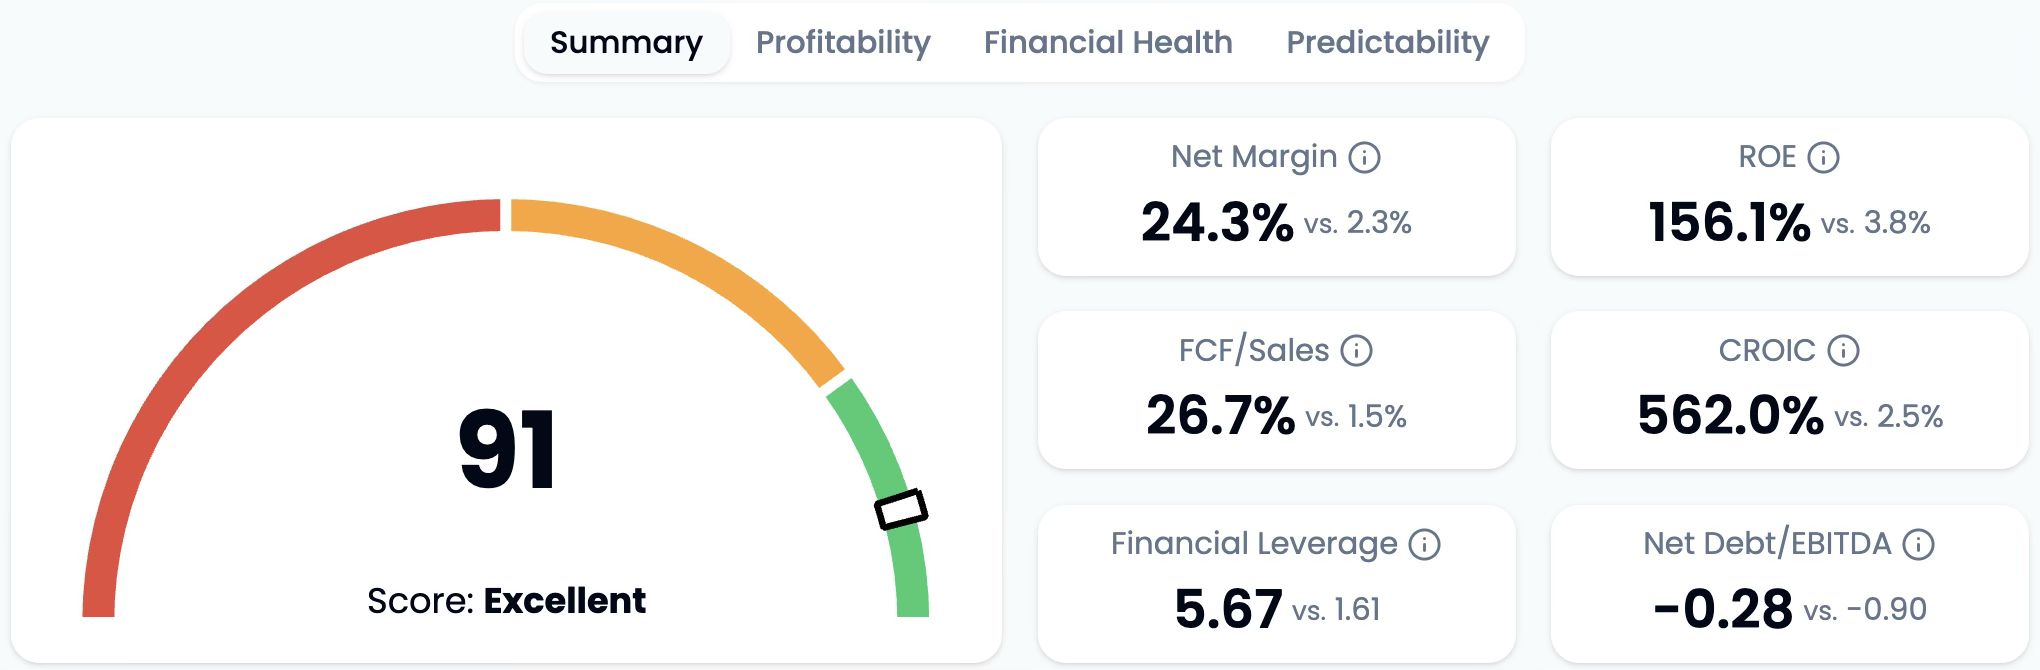
\includegraphics[width=0.8\textwidth]{images/tweenvest/quality score.png}
    \caption{Tweenvest's Quality Score}
    \label{fig:quality_score}
\end{figure}


\noindent After calculating all of this ratios, Tweenvest compares them to the sectors' median and interpolates each of them to create a single score for the ratio, then it aggregates them all using personalized weights to create the final Quality Score, which is then showed to the clients as shown in Figure \ref{fig:quality_score}.


\subsection{Growth}
\noindent The Growth Score evaluates a company's historical growth across multiple key metrics, and compares them to industry standards. This comprehensive approach ensures a balanced assessment of growth across different aspects of the business:

\subsubsection{Revenue \& Profitability Growth}
\begin{itemize}
    \item \textbf{Sales}: Measures growth in core revenue streams
    \item \textbf{EBITDA}: Captures growth in operational cash-generating ability before non-cash and financing impacts
    \item \textbf{Operating Income}: Reflects growth in profit from core business operations
    \item \textbf{Net Income}: Includes all income sources, showing overall profitability growth
\end{itemize}

\subsubsection{Cash Flow Growth}
\begin{itemize}
    \item \textbf{Operating Cash Flow}: Measures growth in cash generation from operations
    \item \textbf{Simple FCF}: A straightforward proxy for available cash after essential investments
    \item \textbf{Levered/Unlevered FCF}: Provide detailed views of free cash flow with and without debt impact
    \item \textbf{Owner Earnings}: Useful for volatile capex cases, emphasizing cash available to shareholders
\end{itemize}

\subsubsection{Capital Base Expansion}
\begin{itemize}
    \item \textbf{Total Assets}: Indicates expansion in overall asset base
    \item \textbf{Equity}: Reflects growth in shareholders' claim on the business
    \item \textbf{Tangible Book Value}: Highlights growth in physical net assets, excluding intangibles
    \item \textbf{Invested Capital}: Captures total capital being put to productive use
    \item \textbf{Capital Employed}: A broader measure of capital supporting business operations
\end{itemize}

\subsubsection{Per-Share Value Growth}
\begin{itemize}
    \item \textbf{Diluted EPS}: Tracks per-share earnings growth, accounting for dilution effects
    \item \textbf{Diluted Shares}: Included to track share count changes, ensuring EPS growth isn't artificially inflated by buybacks or dilution
    \item \textbf{Ordinary DPS}: Tracks the growth of shareholder payouts, a proxy for confidence in future earnings
\end{itemize}

\vspace{0.5cm}
\noindent To compute the Growth Score, Tweenvest calculates 10-year, 5-year, and 3-year averages and then interpolates the growth rate to industry standards. This approach reinforces the long-term investment philosophy, giving lasting growing companies a better score.

\begin{figure}[H]
    \centering
    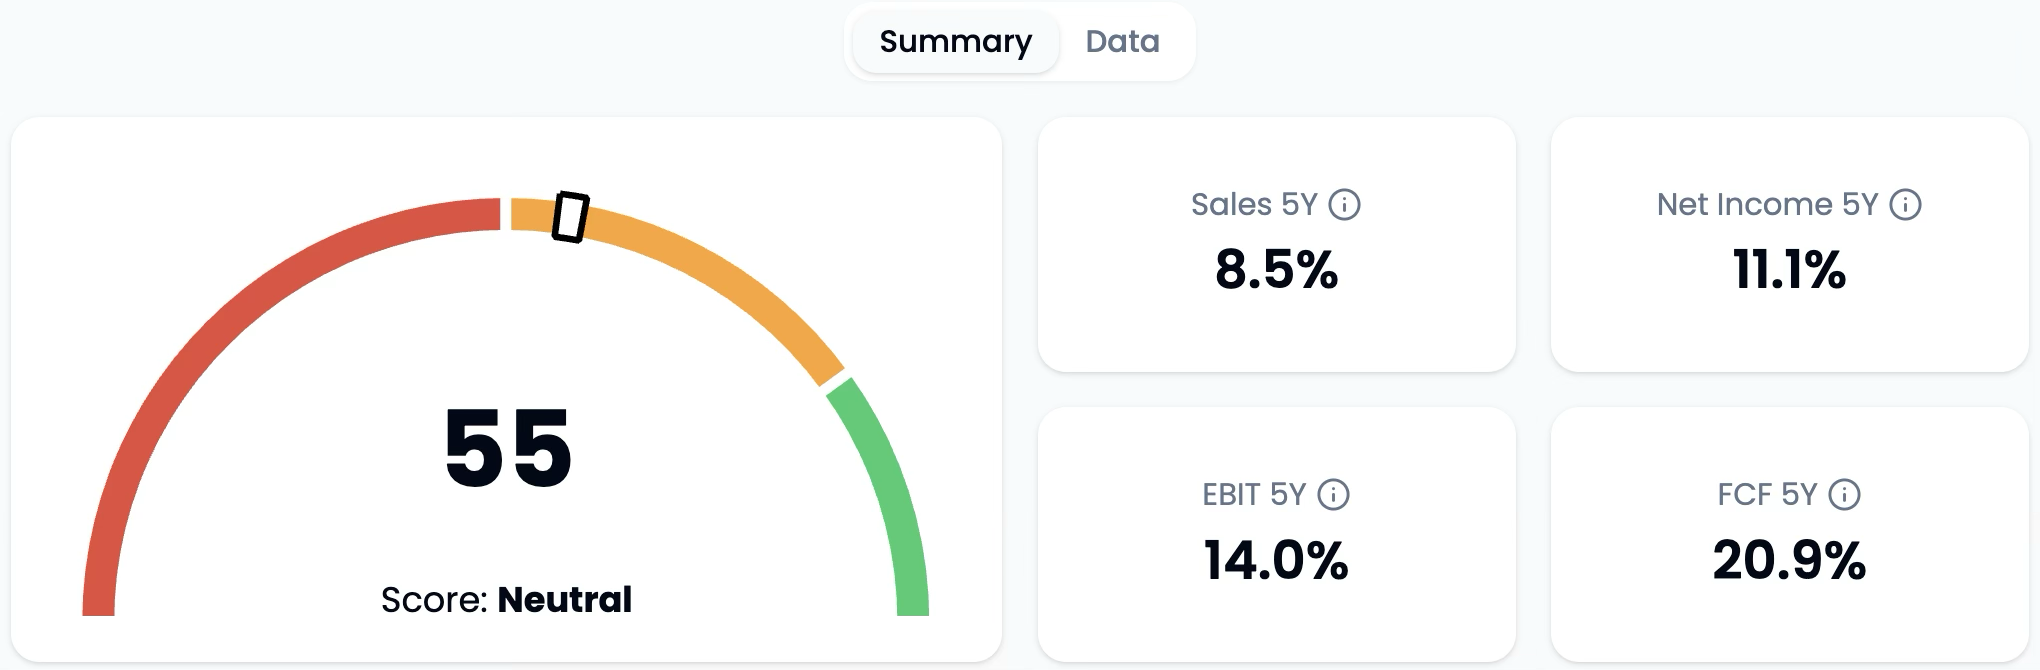
\includegraphics[width=0.8\textwidth]{images/tweenvest/growth score.png}
    \caption{Tweenvest's Growth Score}
    \label{fig:growth_score}
\end{figure}

\subsection{Value}
\noindent The Value Score measures how attractively a company is priced relative to fundamental multiples such as earnings, cash flow, sales, and dividends. This is critical for investors following value investing principles, where the goal is to buy quality companies for less than their intrinsic worth. The algorithm evaluates a series of valuation multiples—both price-based and enterprise value-based—and dividend yield.

% TODO: TTM capital definitions

\subsubsection{Price-Based Multiples}
\begin{itemize}
    \item \textbf{P/E} (Market Cap / Adjusted TTM Earnings): Measures how much investors are willing to pay per dollar of earnings
    \item \textbf{P/S} (Market Cap / TTM Revenue): Useful when earnings are volatile; shows valuation relative to sales
    \item \textbf{P/CF} (Market Cap / TTM Operating Cash Flow): Reflects valuation relative to cash-generating ability
    \item \textbf{P/B} (Market Cap / Tangible Equity): Especially relevant for asset-heavy sectors like banks or industrials
\end{itemize}

\subsubsection{Enterprise Value-Based Multiples}
\begin{itemize}
    \item \textbf{EV/Sales} (Enterprise Value / TTM Revenue)
    \item \textbf{EV/EBITDA} (Enterprise Value / TTM EBITDA)
    \item \textbf{EV/EBIT} (Enterprise Value / TTM EBIT)
    \item \textbf{EV/FCF} (Enterprise Value / TTM Free Cash Flow)
\end{itemize}

\subsubsection{Yield-Based Valuation}
\begin{itemize}
    \item \textbf{Dividend Yield (\%)} (Dividend per Share / Price per Share)
\end{itemize}

\vspace{0.5cm}
\noindent Each of these ratios is compared to multiple historical statistics and sector benchmarks to create individual scores and then average them.

\vspace{0.5cm}
\noindent \textbf{Note:}
\begin{itemize}
    \item \textit{Market Cap = Share Price × Total Outstanding Shares}
    \item \textit{Enterprise Value = Market Capitalization + Total Debt - Cash + Marketable Securities}
\end{itemize}

\begin{figure}[H]
    \centering
    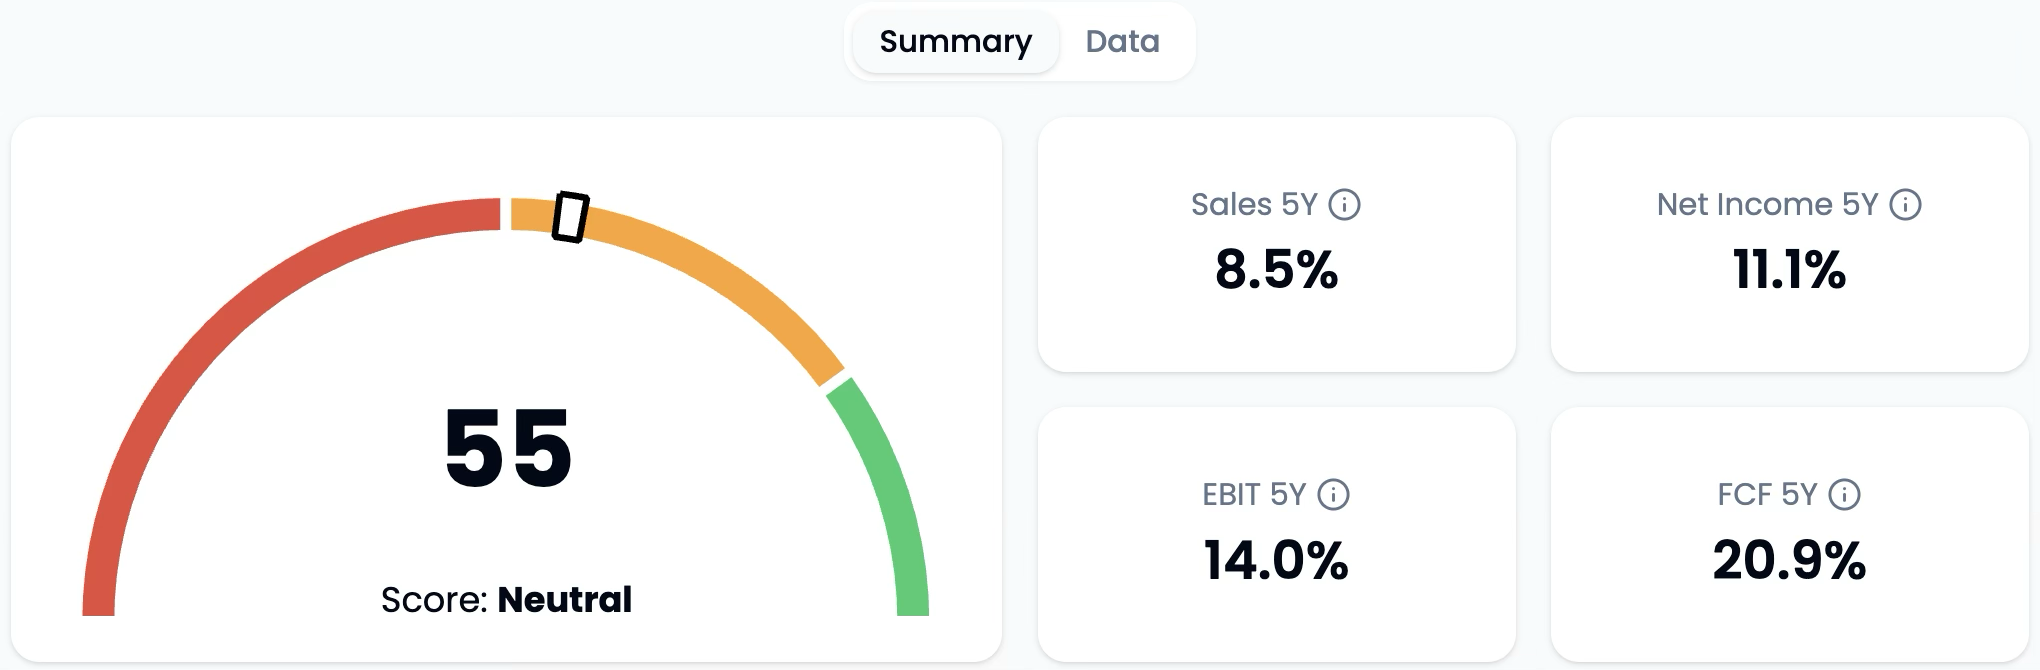
\includegraphics[width=0.8\textwidth]{images/tweenvest/value score.png}
    \caption{Tweenvest's Value Score}
    \label{fig:valuation_score}
\end{figure}


\subsection{Dividend}
\noindent When analyzing Tweenvest most common investors profile, we see a high tendency to income-focused and long-term investors using mainly dividends as their principal concern. Thats why the platform dedicated a full section to this topic. 

\vspace{0.5cm}
\noindent The Dividend Score measures the attractiveness, reliability, and growth potential of a company's dividend payments. It helps investors assess whether the dividend is both rewarding today and sustainable for tomorrow. To do so, the score was built from three primary components:

\subsubsection{Safety}
This part of the score is used to assess the sustainability of the dividend.
\begin{itemize}
    \item \textbf{Payout Ratio EPS} (DPS / Diluted EPS): Shows if dividends are covered by accounting earnings
    \item \textbf{Payout Ratio FCF} (DPS / Free Cash Flow per Share): Shows if dividends are funded by real cash generation
    \item \textbf{Payout Ratio Owner Earnings} (DPS / Owner Earnings per Share): A conservative test of sustainability (excludes CAPEX)
\end{itemize}

\subsubsection{Growth}
\noindent Measures how consistently and strongly the dividend has grown over time.
\begin{itemize}
    \item \textbf{Ordinary DPS CAGR}: 3-Year, 5-Year, 10-Year growth rates
\end{itemize}

\subsubsection{Yield}
\noindent This evaluates the attractiveness of the dividend today relative to the company's historical averages and sector benchmarks.
\begin{itemize}
    \item \textbf{Dividend Yield} (DPS / Price per Share): Represents how much income an investor receives annually from dividends
\end{itemize}

\vspace{0.5cm}
\noindent These components are individually scored weighted and interpolated against industry benchmarks to form a composite score. 

\begin{figure}[H]
    \centering
    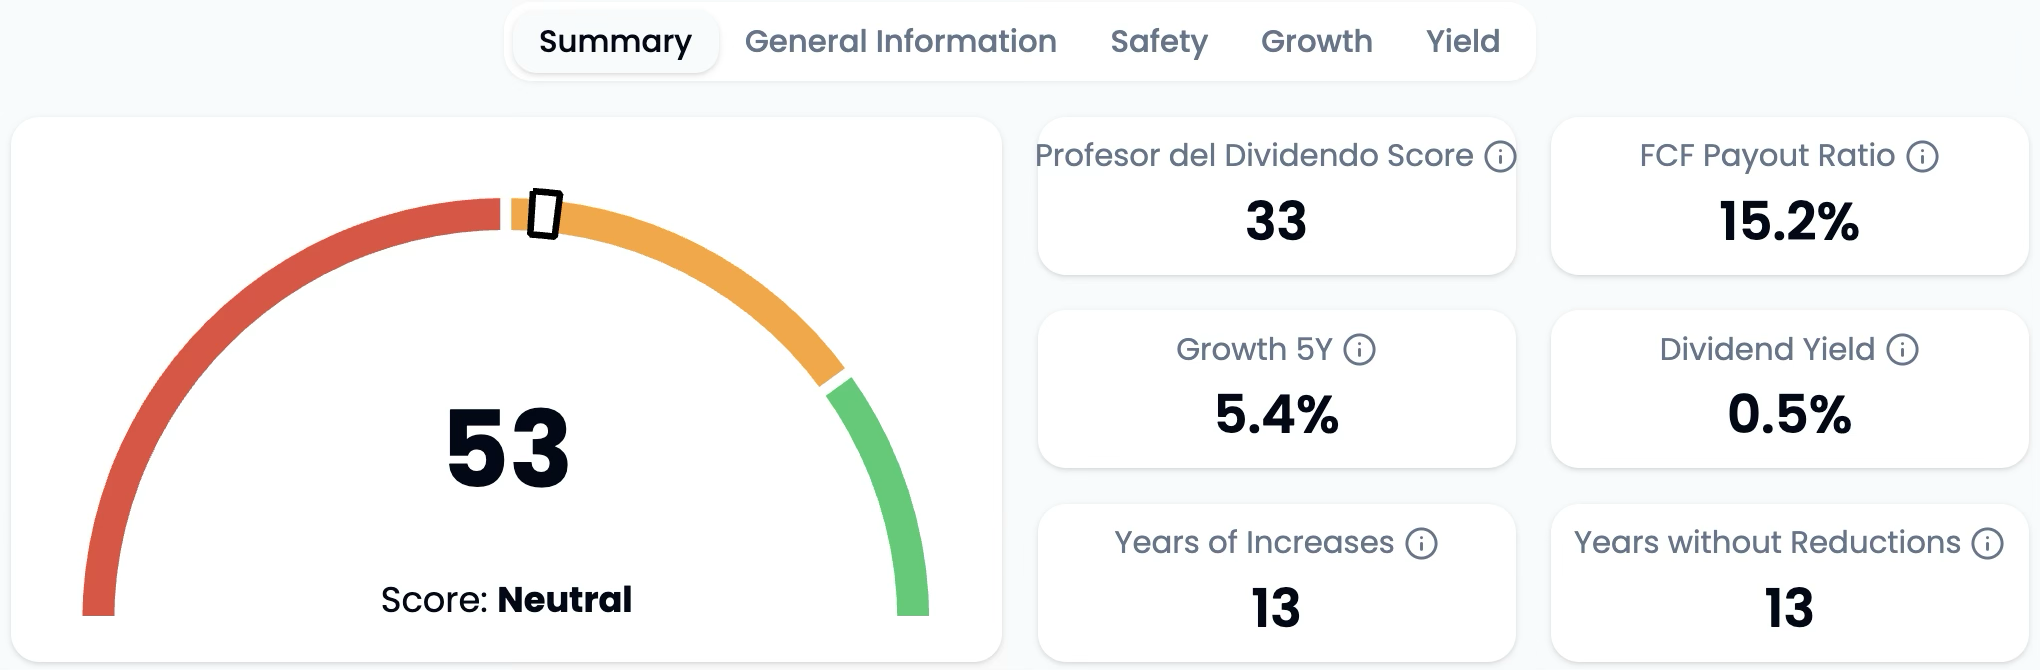
\includegraphics[width=0.8\textwidth]{images/tweenvest/dividend score.png}
    \caption{Tweenvest's Dividend Score}
    \label{fig:dividend_score}
\end{figure}

\noindent Finally, as seen in Figure \ref{fig:dividend_score}, the algorithm adjusts this score based on how many years the dividend has been maintained or increased, \textbf{rewarding consistency}.

\section{Code practices}
Since the code that needs to be changed is used in a production environment by Tweenvest, it is important to follow some \textit{good practices} to ensure the code is easy to understand, maintain, and to avoid introducing new bugs.

\begin{itemize}
  \item \textbf{Understanding and Documenting}: Before starting to work on the code, it is important to understand the codebase and the purpose of the code. For this, it is recommended to use some tools like flux diagrams, code comments, and documentation. As it will be shown later on.
  \item \textbf{Testing}: To ensure proper functionality, every function and class should have unit tests that cover all possible scenarios. These tests are run automatically by the CI/CD pipeline.
  \item \textbf{Pair code review}: After completing the previous steps, the code undergoes a pair code review process, where at least one other team member reviews and approves the changes in \textit{Github} before merging into the main branch.
  \item \textbf{Logging}: After each feature is implemented, it is important to analyze the actual performance in the production environment by looking at its logs to check if the feature is working as expected, and to look for any possible optimizations to be made.
\end{itemize}

\section{Preprocessing}

Once we have created our raw dataset, we need to inspect it and make sure it is consistent and ready to be used for the modeling. This part is really important to avoid any bias in the modeling process and to only use the data that is actually relevant for the analysis.

\subsection{Data Consistency}

Since all of the data is coming from a data provider that uses OCR as one of their tools whenever they don't have the data in a structured format, we need to be very restrictive with the data used. Also, as we mentioned before, some of the algorithms for calculating the scores use long-term data such as 10 year growths rates.

\vspace{0.5cm}
\noindent This is one of the biggest \textbf{limitations to the study}: we will be missing the data of companies that stopped existing or that were acquired by other companies, if they didn't exist for 10 or more years.

\vspace{0.5cm}
\noindent For inspecting the data, we will use the \textit{pandas} \cite{pandas2024}, \textit{matplotlib} \cite{matplotlib2025doc}, and \textit{seaborn} \cite{seaborn2024}, which are powerful tools for data manipulation and analysis. The focus will be on the following aspects:
\begin{itemize}
  \item \textbf{Missing Values}: We need to check if there are any missing values in the data.
  \item \textbf{Data Distributions}: We need to make sure that the data is distributed in a way that is suitable for the modeling.
  \item \textbf{Variable Correlations}: We also have to see if there are any correlations between the variables. For this, we will use the correlation matrix defined as:
  \begin{equation}
    \rho_{X,Y} = \frac{\text{Cov}(X,Y)}{\sigma_X \sigma_Y}
  \end{equation}
  where \(\text{Cov}(X,Y)\) is the covariance between the variables \(X\) and \(Y\), \(\sigma_X\) is the standard deviation of \(X\), and \(\sigma_Y\) is the standard deviation of \(Y\). This matrix will be created with a custom heatmap function (see Appendix~\ref{app:custom_functions}).
  \item \textbf{Data Patterns}: We need to check if there are any visible data patterns between the variables. To address this, we will use a custom \textit{pairplot} function from \textit{seaborn}, which is a powerful tool for data visualization and exploration  depending on the type of variable (see Appendix~\ref{app:custom_functions}).
\end{itemize}

\vspace{0.5cm}
\noindent Additionally, we decided to assign a value of 0 to all null Dividend scores, as a null value indicates that the company does not pay dividends. This choice was made to ensure that the Dividend score remains part of the analysis when evaluating its relevance to long-term profitability, rather than being excluded due to missing values.


% ############################### PREPROCESSING #######################
\subsection{Data Transformation}

To ensure a robust and well-performing model, it is often necessary to transform the data into a format more suitable for learning algorithms, with the obligatory condition of being able to revert it back to its original scale when needed. 

\vspace{0.5cm}
\noindent This step is particularly important because many components of machine learning models—such as the RBF kernel in Support Vector Machines or the regularization terms (L1 and L2) in linear models—implicitly assume that features are centered around zero and have comparable variances. Without this adjustment, features with significantly larger variances could dominate the optimization process, leading the model to underweight or ignore more informative but lower-variance features.

\subsubsection{Standard Scaler}
When training the neural networks, it is really important to standardize the data. We can easily use the \textit{StandardScaler} from the \textit{scikit-learn} library that transforms a feature \(x_i\) with the following formula:

\begin{equation}
z_i = \frac{x_i - \mu}{\sigma}
\end{equation}

\noindent where \(\mu\) is the mean of the feature and \(\sigma\) is its standard deviation. This transformation results in a distribution with a mean of 0 and a standard deviation of 1.



\subsubsection{Gaussian Transformation}

In numerous modeling applications, having normally distributed features is advantageous. \textbf{Power transformations} represent a set of parametric, monotonic functions that are an extension of the Box-Cox transformation. They are designed to convert data from various distributions into approximately Gaussian distributions, thereby reducing variance fluctuations and decreasing distribution asymmetry. 

\vspace{0.5cm}
\noindent We decided to use the \textbf{Yeo-Johnson transformation} because it allows for negative values and it is reversible.

\begin{equation}
x_i^{(\lambda)} =
\begin{cases}
\frac{[(x_i + 1)^\lambda - 1]}{\lambda}, & \text{if } x_i \geq 0, \lambda \neq 0 \\
\ln(x_i + 1), & \text{if } x_i \geq 0, \lambda = 0 \\
-\frac{[(-x_i + 1)^{2 - \lambda} - 1]}{2 - \lambda}, & \text{if } x_i < 0, \lambda \neq 2 \\
-\ln(-x_i + 1), & \text{if } x_i < 0, \lambda = 2
\end{cases}
\end{equation}

\noindent Where \(\lambda\) is a power parameter that helps minimize the skewness of the data. And since we have already deleted extreme outliers, the final distribution shouldn't be too distorted.

\vspace{0.5cm}

\noindent Here are some exammples of the transformations for different distributions:

\begin{figure}[H]
    \centering
    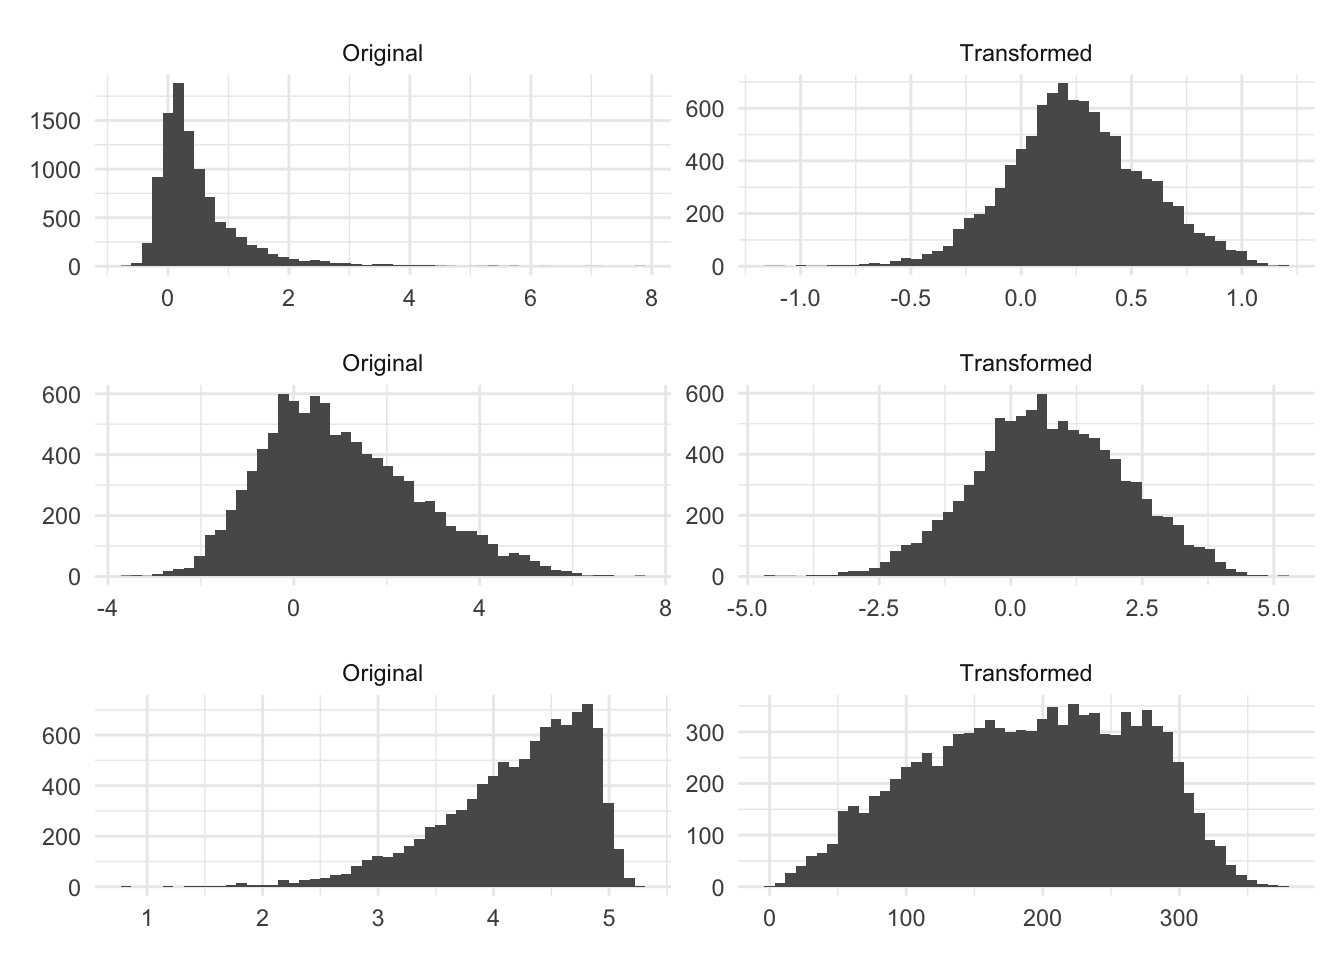
\includegraphics[width=0.8\textwidth]{images/code/transformations/yeo-johnson.png}
    \caption{Yeo-Johnson Transformations examples}
    \label{fig:yeo-johnson}
\end{figure}


\section{Outlier Detection}

Anomalies are data patterns that have different data characteristics from normal
instances. The ability to detect anomalies has significant relevance since often provide critical and actionable information in many different contexts.

\vspace{0.5cm}
\noindent For example, anomalies in credit card transactions could signify fraudulent use of
credit cards, or an unusual computer network traffic pattern could stand for an
unauthorised access.


\subsection{Inter Quartile Range}

Given a univariate dataset, the Interquartile Rule identifies outliers based on the interquartile range (IQR). The steps are as follows:

\begin{enumerate}
    \item Compute the first quartile ($Q_1$), which is the 25th percentile of the data.
    \item Compute the third quartile ($Q_3$), which is the 75th percentile of the data.
    \item Calculate the interquartile range:
    \[
        \text{IQR} = Q_3 - Q_1
    \]
    \item Define the lower and upper bounds for non-outlier values following the 1.5 rule:
    \[
        \text{Lower bound} = Q_1 - 1.5 \times \text{IQR}
    \]
    \[
        \text{Upper bound} = Q_3 + 1.5 \times \text{IQR}
    \]
    \item Any data point $x$ is considered an outlier if:
    \[
        x < \text{Lower bound} \quad \text{or} \quad x > \text{Upper bound}
    \]
\end{enumerate}

\noindent As we can see this is a very simple and intuitive method, but it has some limitations:

\begin{table}[H]
    \centering
    \begin{tabular}{|p{7cm}|p{7cm}|}
    \hline
    \textbf{Pros} & \textbf{Cons} \\
    \hline
    Simple to compute and interpret. & Not suitable for multivariate data with correlated features. \\
    \hline
    Non-parametric. & May misclassify values in skewed distributions as outliers. \\
    \hline
    Robust to extreme values, since it relies on percentiles rather than the mean. & Fixed multiplier is arbitrary and may need tuning for each dataset. \\
    \hline
    \end{tabular}
    \caption{Pros and Cons of the Interquartile Rule}
\end{table}

\noindent Even though this method is simple to compute and interpret, it is not suitable for multivariate data with correlated features, and that's where the rest of the methods come into play.

\subsection{Single Vector Machine}

\noindent Support Vector Machines (SVMs) represent a robust class of unsupervised learning algorithms that can be effectively adapted for anomaly detection tasks. This algorithm establishes itself on the premise that the majority of real-world data is inherently normal. Where the goal is to define a boundary encapsulating the normal instances in the feature space, thereby creating a region of familiarity. 

\vspace{0.5cm}
\noindent To capture the bases of the \textit{scikit-learn} implementation \cite{scikit2025oneclasssvm} used in this work, we can say that the main idea is to find a minimum volume sphere that contain all the training samples. This sphere, described by its center \(c\) and its radius \(r\), is obtained by solving the constrained optimization problem: \cite{zineb2012simple}
\begin{equation}
\min_{r,c} r^2 \quad \text{subject to} \quad \|\Phi(x_i) - c\|^2 \leq r^2 \quad \text{for} \quad i = 1, 2, \ldots, n
\end{equation}

\vspace{0.5cm}
\noindent This boundary is strategically positioned to maximize the margin around the normal data points, allowing for a clear delineation between what is considered ordinary and what may be deemed unusual. This emphasis on margin maximization is akin to creating a safety buffer around the normal instances, fortifying the model against the influence of potential outliers or anomalies.

\vspace{0.5cm}
\noindent In summary, this method has the following characteristics:

\begin{table}[H]
    \centering
    \begin{tabular}{|p{7cm}|p{7cm}|}
        \hline
        \textbf{Pros} & \textbf{Cons} \\
            \hline
            Effective for high-dimensional data and complex boundaries. & Sensitive to the choice of kernel and hyperparameters (e.g., $\nu$, $\gamma$). \\
            \hline
            Works well when the training set contains mostly or only normal instances. & Computationally intensive, especially on large datasets. \\
            \hline
            Can capture nonlinear patterns using kernels (e.g., RBF kernel). & Difficult to interpret or explain the decision function. \\
            \hline
            No need for labeled data from the outlier class. & -- \\
            \hline
            Solid theoretical foundation and widely supported in machine learning libraries. & -- \\
        \hline
    \end{tabular}
    \caption{Pros and Cons of One-Class SVM for Outlier Detection}
\end{table}
    
    
\subsection{Isolation Forest}

As we are seeing in this small fraction of outlier detection methodologies, most of the existing anomaly detection approaches are based on the premise of normal distributions, then identify anomalies as those that do not conform to the normal profile.

\vspace{0.5cm}
\noindent But to solve this issue we can use the Isolation Forest algorithm, which is explained in the original paper \textcite{liu2012isolation}. The algorithm constructs multiple isolation binarytrees (iTrees) from the dataset, where anomalies are identified as data points that exhibit shorter average path lengths across these trees.

\vspace{0.5cm}
\noindent Lets consider a dataset $X = \{x_1, \dots, x_n\}$ containing $n$ points in $d$-dimensional space, and a subset $X' \subset X$. An Isolation Tree (iTree) is constructed as follows:

\begin{itemize}
    \item Each node $T$ in the tree is either:
    \begin{itemize}
        \item An external node (leaf) with no children, or
        \item An internal node with exactly two children ($T_l$ and $T_r$) and a test condition
    \end{itemize}
    \item The test condition at each internal node consists of:
    \begin{itemize}
        \item A randomly selected attribute $q$
        \item A split value $p$
        \item A test $q < p$ that determines whether a point goes to $T_l$ or $T_r$
    \end{itemize}
\end{itemize}

\noindent The tree construction process recursively partitions $X'$ by randomly selecting attributes and split values until either:
\begin{itemize}
    \item The node contains only one instance, or
    \item All instances at the node have identical values
\end{itemize}
\begin{figure}[H]
    \centering
    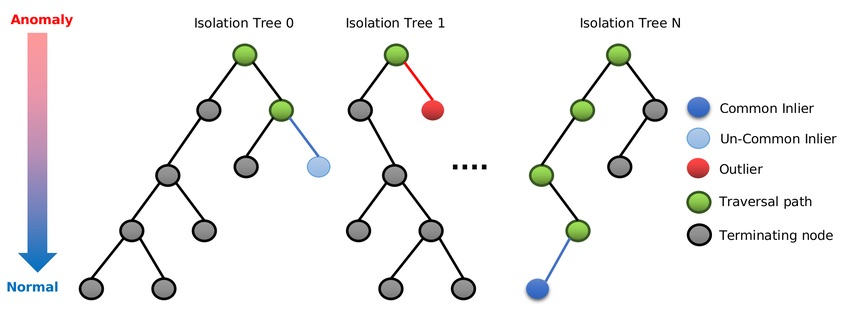
\includegraphics[width=0.8\textwidth]{images/code/outliers/IF.jpeg}
    \caption{Visualization of how Isolation Forest works.}
    \label{fig:isolation_forest}
\end{figure}

\noindent As we can see in Figure \ref{fig:isolation_forest}, once the iTree is fully constructed, each point $x_i \in X$ is isolated at a leaf node. The path length $h(x_i)$ of a point $x_i$ is defined as the number of edges traversed from the root to its leaf node. Points with shorter path lengths are considered more likely to be anomalies, as they require fewer splits to be isolated from the rest of the data.

\noindent This method works very good in most cases, but it has also its own limitations:

\begin{table}[H]
    \centering
    \begin{tabular}{|p{7cm}|p{7cm}|}
    \hline
    \textbf{Pros} & \textbf{Cons} \\
    \hline
    Efficient and scalable to large datasets due to its tree-based structure. & Less effective for detecting local outliers in densely clustered regions. \\
    \hline
    Non-parametric: does not assume any data distribution. & Performance can vary with the choice of parameters like number of estimators and subsample size. \\
    \hline
    Naturally handles high-dimensional data. & Not suitable for detecting subtle anomalies that closely resemble normal data. \\
    \hline
    Requires little preprocessing (no need for feature scaling). & -- \\
    \hline
    Robust to irrelevant features due to random sub-sampling. & -- \\
    \hline
    \end{tabular}
    \caption{Pros and Cons of the Isolation Forest Method for Outlier Detection}
\end{table}

\subsection{Local Outlier Factor}

Since we are looking at outliers from the perspective of correlations between the different response variables to see which companies don't behave naturally. We also checked on the Local Outlier Factor (LOF) for being based on hyper-plane densities of data.

\vspace{0.5cm}
\noindent The algorithm measures the local deviation of the density of a given sample with respect to its neighbors. It is local in that the anomaly score depends on how isolated the object is with respect to the surrounding neighborhood. More precisely, locality is given by k-nearest neighbors, whose distance is used to estimate the local density. By comparing the local density of a sample to the local densities of its neighbors, one can identify samples that have a substantially lower density than their neighbors. These are considered outliers. \textcite{breunig2000lof}


\begin{table}[H]
    \centering
    \begin{tabular}{|p{7cm}|p{7cm}|}
    \hline
    \textbf{Pros} & \textbf{Cons} \\
    \hline
    Can detect outliers relative to their local neighborhood, allowing it to identify context-specific anomalies. & LOF scores are relative and lack a universal interpretation threshold for outliers. \\
    \hline
    Effective in datasets with varying densities — unlike global methods, it can recognize outliers near dense clusters. & Sensitivity to parameter selection (e.g., number of neighbors) can affect performance and consistency. \\
    \hline
    Applicable in any domain where a dissimilarity measure is defined, not limited to vector spaces. & Not inherently scalable to very large datasets without approximation or optimization. \\
    \hline
    Works well across domains, such as network intrusion detection or classification tasks. & -- \\

    \hline
    Easily generalizable and adaptable for use in spatial data, temporal data, and network structures. & -- \\
    \hline
    \end{tabular}
    \caption{Pros and Cons of the Local Outlier Factor (LOF) Method}
\end{table}
    
\subsection{Multi-Criteria Outlier Detection}

There is a big controversy in the field about the best method to detect the outliers, since the results can vary a lot depending on the algorithm used.

\vspace{0.5cm}
\noindent So to attempt to fix this issue, after reading some aggregative methods such as \textcite{abro2020stacking}, we created a multi-modal method that combines the results of the different methods to get a more robust result.

\begin{figure}[H]
    \centering
    \includegraphics[width=1\textwidth]{images/code/outliers/multimodal.png}
    \caption{Multi-Criteria Outlier Detection Method}
    \label{fig:multimodal}
\end{figure}


\vspace{0.5cm}
\noindent As shown in the Figure \ref{fig:multimodal}, this starts by homogenizing the variables distribution with a common data transformation so they are more Normal, but to make sure that the final data isn't being transformed we copy the original dataset earlier. After this, we use multiple methods to detect the different outliers and then we make the intersection between them to get the common outliers. By the end of this process we have tagged the original dataset rows, assuring that the data that will be excluded is only formed by \textit{"true outliers"}.

%TODO: maybe move this to the results section
\vspace{0.5cm}
\noindent We noticed that since this method is very restrictive, we have to set a threshold multiplier to the original dataset to get the final outliers. So for example, a 20\% threshold would only exclude around 4\% of the original dataset because of the intersection of all the methods makes it very restrictive. Here we \textbf{propose for future work} to fine tune the different thresholds for each method to get a more robust result.


% ############################### PREDICTIVE MODELS #######################
\section{Predictive Models}
The main objective of this thesis is to check if the scores have any relation with the future profits of the companies. For doing this in the most generalized way, instead of creating a portfolio following some subjective criteria on the scores, markets and other variables, we used predictive modeling to check for the actual relationships between the response variables and the explanatory ones.

\vspace{0.5cm}
\noindent As a first approach, we created a set of models that separate the scores and the different returns. 


\subsection{Regression Models}

To create the econometrical models, we want to be able to understand the actual relationship between the response variables and the explanatory ones. For this we started with the creation of multiple regression models.

\subsubsection{Linear Regression}

As for the first models, we created a series of linear regression models for each factor score that
includes the interactions between the dummy variables and the score used in each model.

\begin{equation}
    \hat{P_i}=\beta_0+\beta_1 \cdot S_j + 
\sum_{n=2}^{N}\beta_{n}\cdot D_n + S_j \cdot \sum_{m=N+1}^{M}\beta_{m}\cdot D_m
\end{equation}

\noindent where:
\begin{itemize}
    \item \(P_i\) is the estimated profit for each time horizon \(i\)
    \item \(S_j\) is the score for each factor \(j\)
    \item \(D_{n,m}\) are the dummy variables for the industry and region, where \(D_{n,m} := I_k \cup R_l\)
    \item \(\beta\) are the coefficients that weight each variable.
\end{itemize}

\noindent For fitting the models, we also applied a backward selection to remove the variables that are not statistically significant, using the \textbf{p-value} criterion.

\subsubsection{Generalized Additive Models}

Because the relationships between the variables are not linear, we also used the Generalized Additive Models (GAM) to check if they were able to capture the non-linear relationships between the variables.

\vspace{0.5cm}
\noindent According to \textcite{pygam2018}, GAMs are smooth semi-parametric models that can capture non-linear relationships between variables. They take the form:

\begin{equation}
    g(\mathbb{E}[y|X]) = \beta_0 + f_1(X_1) + f_2(X_2,X_3) + \dots + f_M(X_N)
\end{equation}

\noindent where:
\begin{itemize}
    \item \(X^T = [X_1, X_2, \dots, X_N]\) are the independent variables
    \item \(y\) is the dependent variable.
    \item \(g()\) is the link function that relates the predictor variables to the expected value of the dependent variable.
    \item \(f_m()\) are feature functions built using penalized B-splines, which automatically model non-linear relationships without requiring manual transformation of variables.
\end{itemize}

\noindent In our case, we used pyGAMs LinearGAM since the model gives a Normal error distribution, and an identity link.

\subsection{Time Series}
In the stock market, the prices of the stocks are not independent of each other, they are correlated in the time series and they also have memory on past behavior of the company. This is what is known as \textbf{Momentum}, so companies that have a good past performance are more likely to have a good future performance, and vice versa.

\vspace{0.5cm}
\noindent For this reason, we contemplated two possibilities:

\subsubsection{ARIMA Models}
To take account the profit tendency, we implemented ARIMA models to improve the regression models performance by using the residues of the already fitted model:

\begin{equation}
    P_i = \hat{P_i} + {\varepsilon_i} \quad \longleftrightarrow \quad {\varepsilon_i} \sim ARIMA_i(p,d,q)
\end{equation}

\noindent The ARIMA model is defined as:

\begin{equation}
    \phi_i(B_i)(1 - B_i)^{d_i} \varepsilon_i^t = \theta_i(B_i) \eta_i^t
    \end{equation}
    
    \noindent where for each $i$ profit:
    \begin{itemize}
      \item \(\varepsilon_i^t\) is the residual at time \(t\).
      \item \(\eta_i^t\) is a white noise error term (innovation).
      \item \(B_i\) is the backshift operator, such that \(B \varepsilon_i^t = \varepsilon_i^{t-1}\).
      \item \(\phi_i(B) = 1 - \phi_{i1} B - \phi_{i2} B^2 - \dots - \phi_{ip} B^p\) is the autoregressive (AR) polynomial.
      \item \(\theta_i(B) = 1 + \theta_{i1} B + \theta_{i2} B^2 + \dots + \theta_{iq} B^q\) is the moving average (MA) polynomial.
      \item \(d_i\) is the order of differencing.
    \end{itemize}
    


\subsubsection{Windowed Models}
And for capturing possible memory of the companies behavior in different aspects, we also implemented windowed models that used the last \(N\) scores statistical properties to predict future profits.

\vspace{0.5cm}
\noindent So for each score \(j\), we will calculate the average and the standard deviation of the scores over the last \(N\) periods. Let \(S_j^t\) be the score at time \(t\), then for a window of size \(N\):

\begin{equation}
    \bar{S}_j^N = \frac{1}{N} \sum_{i=t-N+1}^{t} S_j^i
\end{equation}

\noindent where:
\begin{itemize}
    \item \(\bar{S}_j^N\) is the average score over window \(N\) for score \(j\)
    \item \(N\) can be 3 months, 6 months, 1 year, or 2 years.
    \item \(t\) is the current time point
\end{itemize}

\noindent For adding also the deviation from the average, we also calculated the standard deviation of the scores over the same window:

\begin{equation}
    \sigma_j^N = \sqrt{\frac{1}{N} \sum_{i=t-N+1}^{t} (S_j^i - \bar{S}_j^N)^2}
\end{equation}

\noindent These statistical measures will be used as additional features in our predictive models to capture the temporal behavior of each score.

\subsection{Neural Networks}

Finally, for trying to capture the non-linear relationships between all the available variables, including the windowed statistical properties, we will use the Neural Networks.

\section{Back-testing}

In order to assess and compare the modeling techniques employed in this thesis, it is important to have a consistent criteria to evaluate them based on the next requirements:

\subsection{Performance}
The first thing we need to see is if the models are able to detect any relationships between the co-variables and the response variable, and how accurate they are:
\begin{itemize}
    \item \textbf{Prediction Accuracy:} $R^2$ and $R^2_{adjusted}$, these metrics quantify the proportion of variance explained by the model.
    \item \textbf{Accuracy:} RMSE, MAE, which evaluate the errors the model makes when predicting the target variable.
\end{itemize}


\subsection{Consistency and Overfitting}
We check whether the models reflect stable, interpretable patterns in the relationships between scores and alpha. For this, we will use the following techniques:
\begin{itemize}
    \item \textbf{Sign of coefficients:} We will check if the sign of the coefficients remains stable across different time horizons.
    \item \textbf{Shape of functions:} We will check if the shape of the functions remains stable across different time horizons.
    \item \textbf{Number of significant variables:} We will check if the number of significant variables increases with the performance of the models, using the $p-value < 0.2$ criterion.
\end{itemize}

\subsection{Robustness of Results}
The residuals of the models should resemble white noise, indicating the absence of unmodeled structure and valid statistical inference \textcite{enders1948applied}.
\begin{itemize}
    \item \textbf{Mean Value Test:} The mean of the residuals should be close to 0, which is checked with the T-test.
        \begin{itemize}
            \item \textbf{Distribution Plots:} Visualize the distribution of residuals to assess if the mean is centered at zero.
        \end{itemize}
    \item \textbf{Heteroscedasticity Tests:} The variance of the residuals should be constant across all time horizons.
        \begin{itemize}
            \item \textbf{White Test:} Checks for general forms of heteroscedasticity.
            \item \textbf{Breusch-Pagan Test:} Tests whether the variance of the errors depends on the values of the independent variables.
            \item \textbf{F and t tests:} Used to compare variances and means across groups.
            \item \textbf{Distribution Plots:} Visualize residuals versus fitted values to detect patterns in variance.
        \end{itemize}
    \item \textbf{Normality Tests:} The distribution of residuals should follow a Normal distribution.
        \begin{itemize}
            \item \textbf{Shapiro-Wilk Test:} Statistical test for normality.
            \item \textbf{Jarque-Bera Test:} Tests whether sample data have the skewness and kurtosis matching a normal distribution.
            \item \textbf{Q-Q Plots:} Visual tool to compare the quantiles of the residuals to a normal distribution.
            \item \textbf{Distribution Plots:} Visualize the histogram or density of residuals.
        \end{itemize}
    \item \textbf{Autocorrelation Test:} The errors should not be correlated with each other.
        \begin{itemize}
            \item \textbf{Durbin-Watson Test:} Checks for the presence of autocorrelation in the residuals.
            \item \textbf{ACF and PACF Plots:} Visualize the autocorrelation and partial autocorrelation of residuals to detect serial correlation.
        \end{itemize}
\end{itemize}




% \begin{itemize}
%     \item \textbf{Consistency}: The models should display stable relationships between scores and alpha across different time horizons. For example, a score that positively impacts alpha in the short term should not suddenly show a strong negative effect in the long term.
%     \item \textbf{Performance}: The models should predict future profitability or alpha with a reasonable level of accuracy.
%     \item \textbf{Overfitting}: Given the number of explanatory variables, we must ensure the models generalize well and are not fitting noise in the training data.
%     \item \textbf{Robustness of Results}: The residuals of the models should resemble white noise, indicating the absence of unmodeled structure and valid statistical inference.
% \end{itemize}


% \begin{table}[H]
%     \centering
%     \caption{Comparison of Model Requirements and Techniques Used}
%     \label{tab:requirements_vs_techniques}
%     \begin{tabular}{|p{3.5cm}|p{4.5cm}|p{5.5cm}|}
%         \hline
%         \textbf{Requirement} & \textbf{Techniques(s) Used} & \textbf{How the Requirement is Addressed} \\
%         \hline
%         Consistency & Sign of coefficients / shape of functions & We check whether the sign of coefficients or the functional shapes (in GAMs) remain stable across different time horizons, indicating stable patterns. \\
%         \hline
%         Performance & RMSE, MAE, $R^2$ & These metrics evaluate how accurately the model explains or predicts the target variable, capturing both error and fit quality. \\
%         \hline
%         Overfitting & $R^2_{\text{adjusted}}$, number of significant variables & Models with high $R^2$ but low $R^2_{\text{adjusted}}$ are penalized. We also track the number of statistically significant variables to control model complexity. \\
%         \hline
%         Robustness of Results & White noise tests (Mean Value Test; Heteroscedasticity Tests: White Test, Breusch-Pagan Test, F and t tests; Normality Tests: Shapiro-Wilk Test, Jarque-Bera Test; Autocorrelation Test: Durbin-Watson Test) & Check if the residuals are white noise using the following tests: (1) Mean Value Test, (2) Heteroscedasticity Tests (White Test, Breusch-Pagan Test, F and t tests), (3) Normality Tests (Shapiro-Wilk Test, Jarque-Bera Test), and (4) Autocorrelation Test (Durbin-Watson Test). Passing these tests indicates that the model has captured the main signal in the data. \\
%         \hline
%     \end{tabular}
% \end{table}





% ############################### DEVELOPMENT  ###############################
\chapter{Development}

\section{Architecture Enhancement}

% \noindent We have understood the nature of the data, explained the bases of how the scores are calculated, and the code methodologies we will be using. Now we need to create a proper dataset.

% \vspace{0.5cm}
% TODO: add the capitals for DB
\noindent At the current moment of beginning this work, Tweenvest kept a large DB of most of the needed information for creating the dataset. This included all of the price histories, historical currency multipliers to dollar, dividends payed per stock… but when it came to the scores we had a traceability problem.

\vspace{0.5cm}
\noindent For optimizing the costs and structure of the DB, Tweenvest chose to only save the latest score for each company and overwriting it each day when calculating the newest one, which led to the first main task.

\subsection{Updating Tweenvest Code}

After locating where the score calculators are called, we have to understand the code's architecture and the relationships between the different database models to see exactly what needs to be changed. Tweenvest uses Django as the main backend's technology to handle a relational database with PostgreSQL, this is due to the nature of the financial data where one the information is related to another.

\begin{figure}[H]
    \centering
    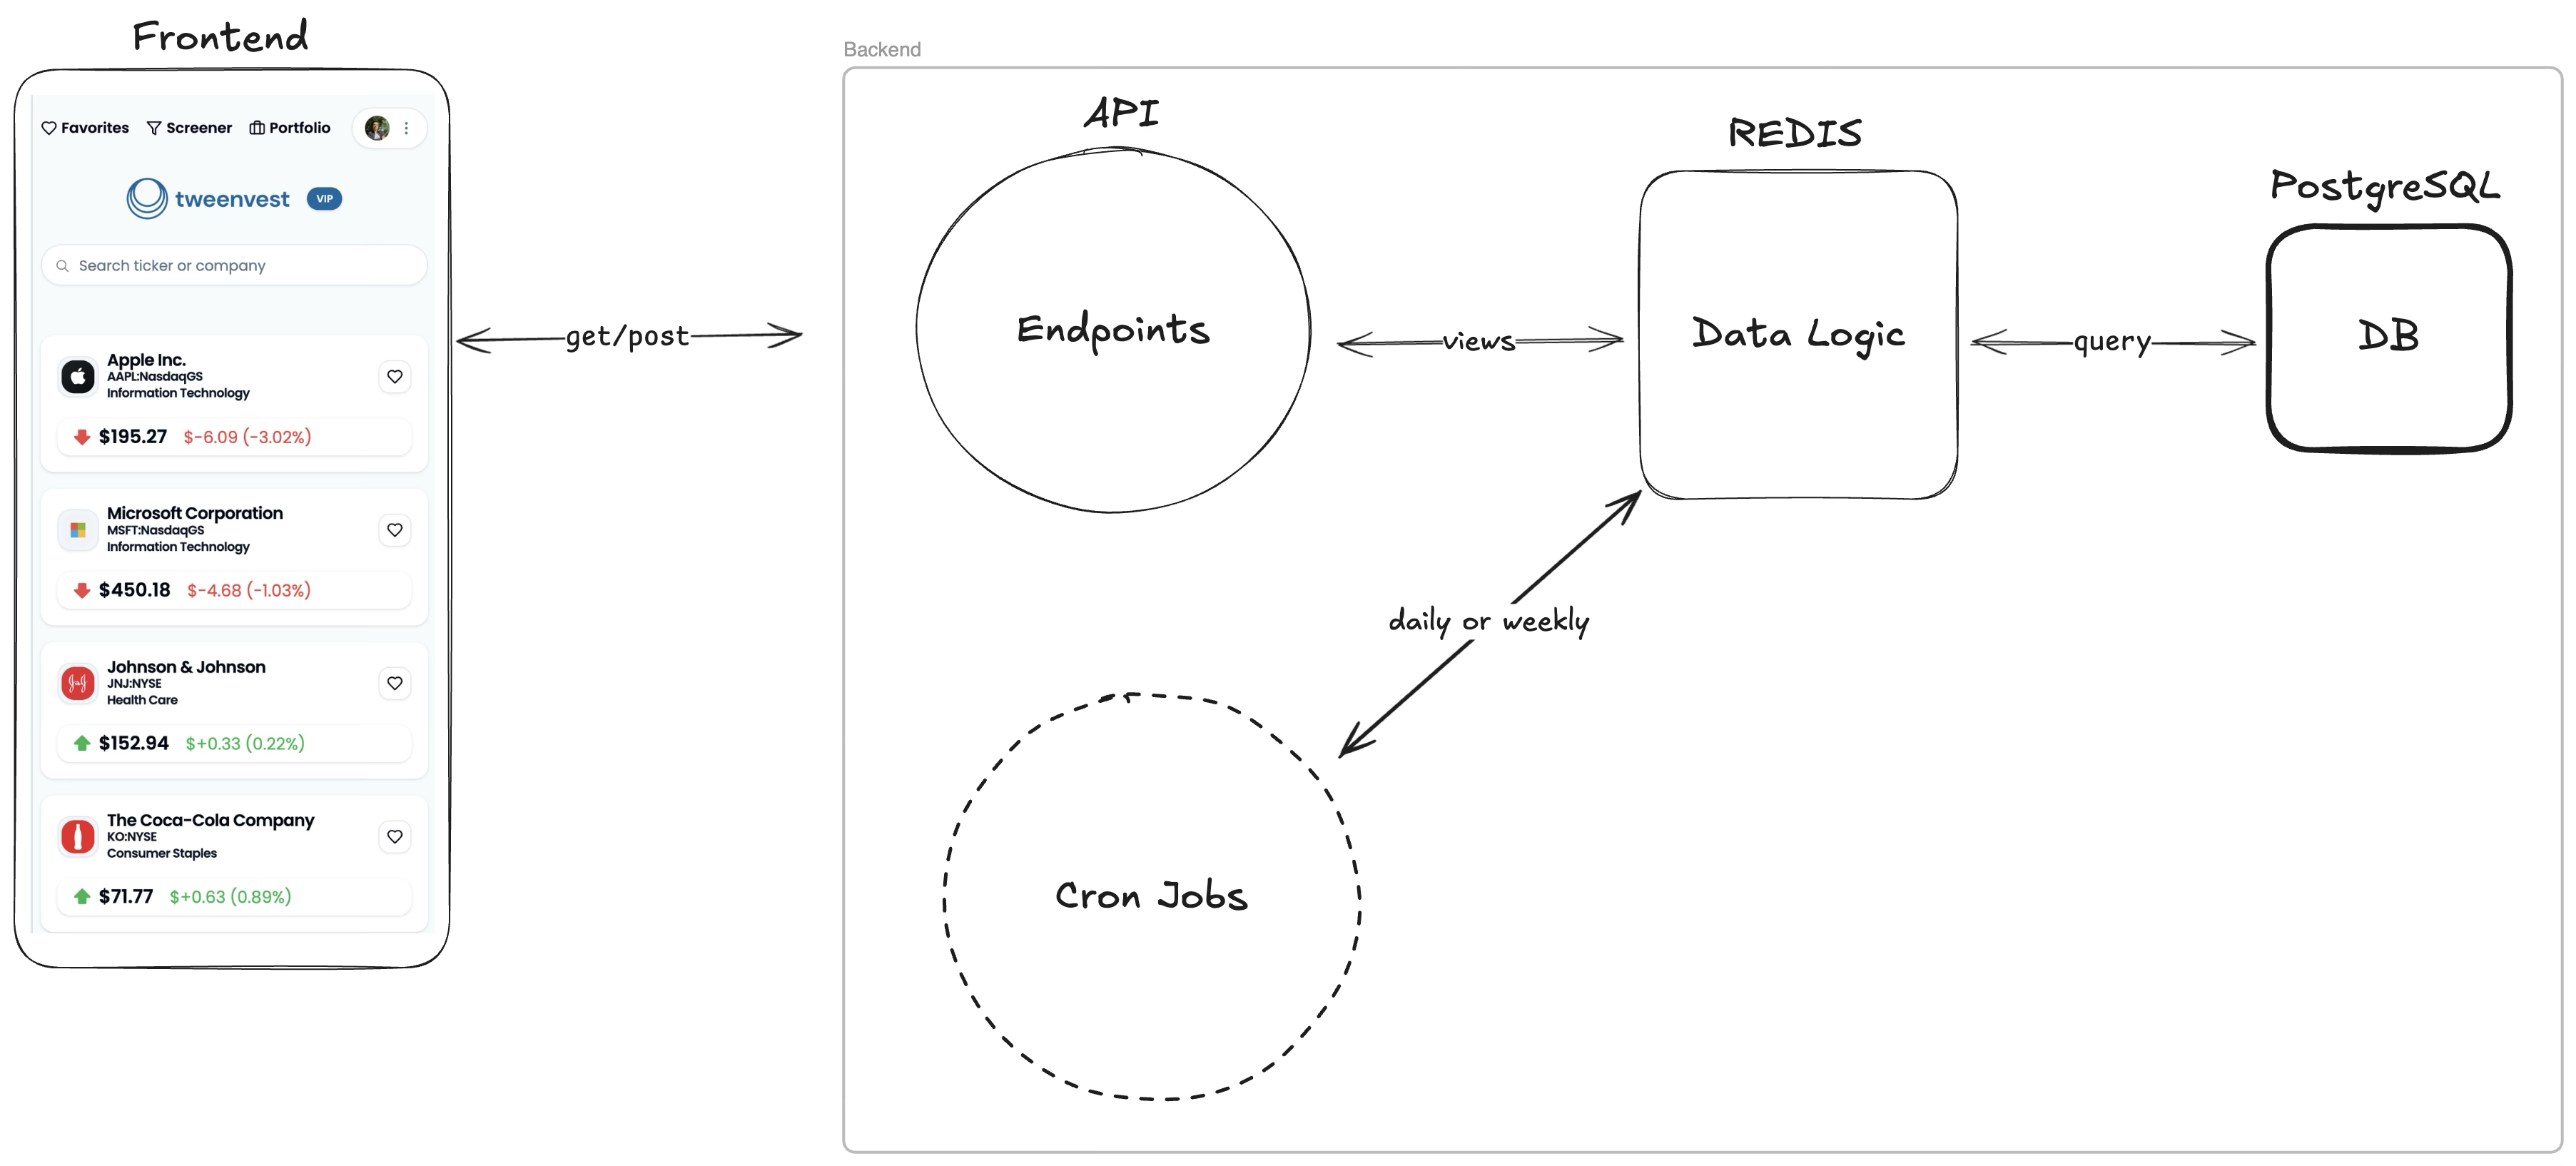
\includegraphics[width=1\textwidth]{images/tweenvest/general architecture.png}
    \caption{General Tweenvest's Architecture}
    \label{fig:general_architecture}
\end{figure}

\noindent As we can see, there are two different actions occurring at the same time. For one side we have all of the requests coming from the users interactions, and for the other hand the programmed jobs that need to be executed every day to update all of the financial information of the stocks, or necessary actions such as sending emails to get authentication pins.

\vspace{0.5cm}
\noindent Since we are changing the data logic for calculating and storing historical data of the factor scores, we need to assure that the systems capabilities don't exceed the platforms needs, and that the changes don't affect the normal calculation of the factor scores, so we had to look at the code corresponding to the factor scores.

\begin{figure}[H]
    \centering
    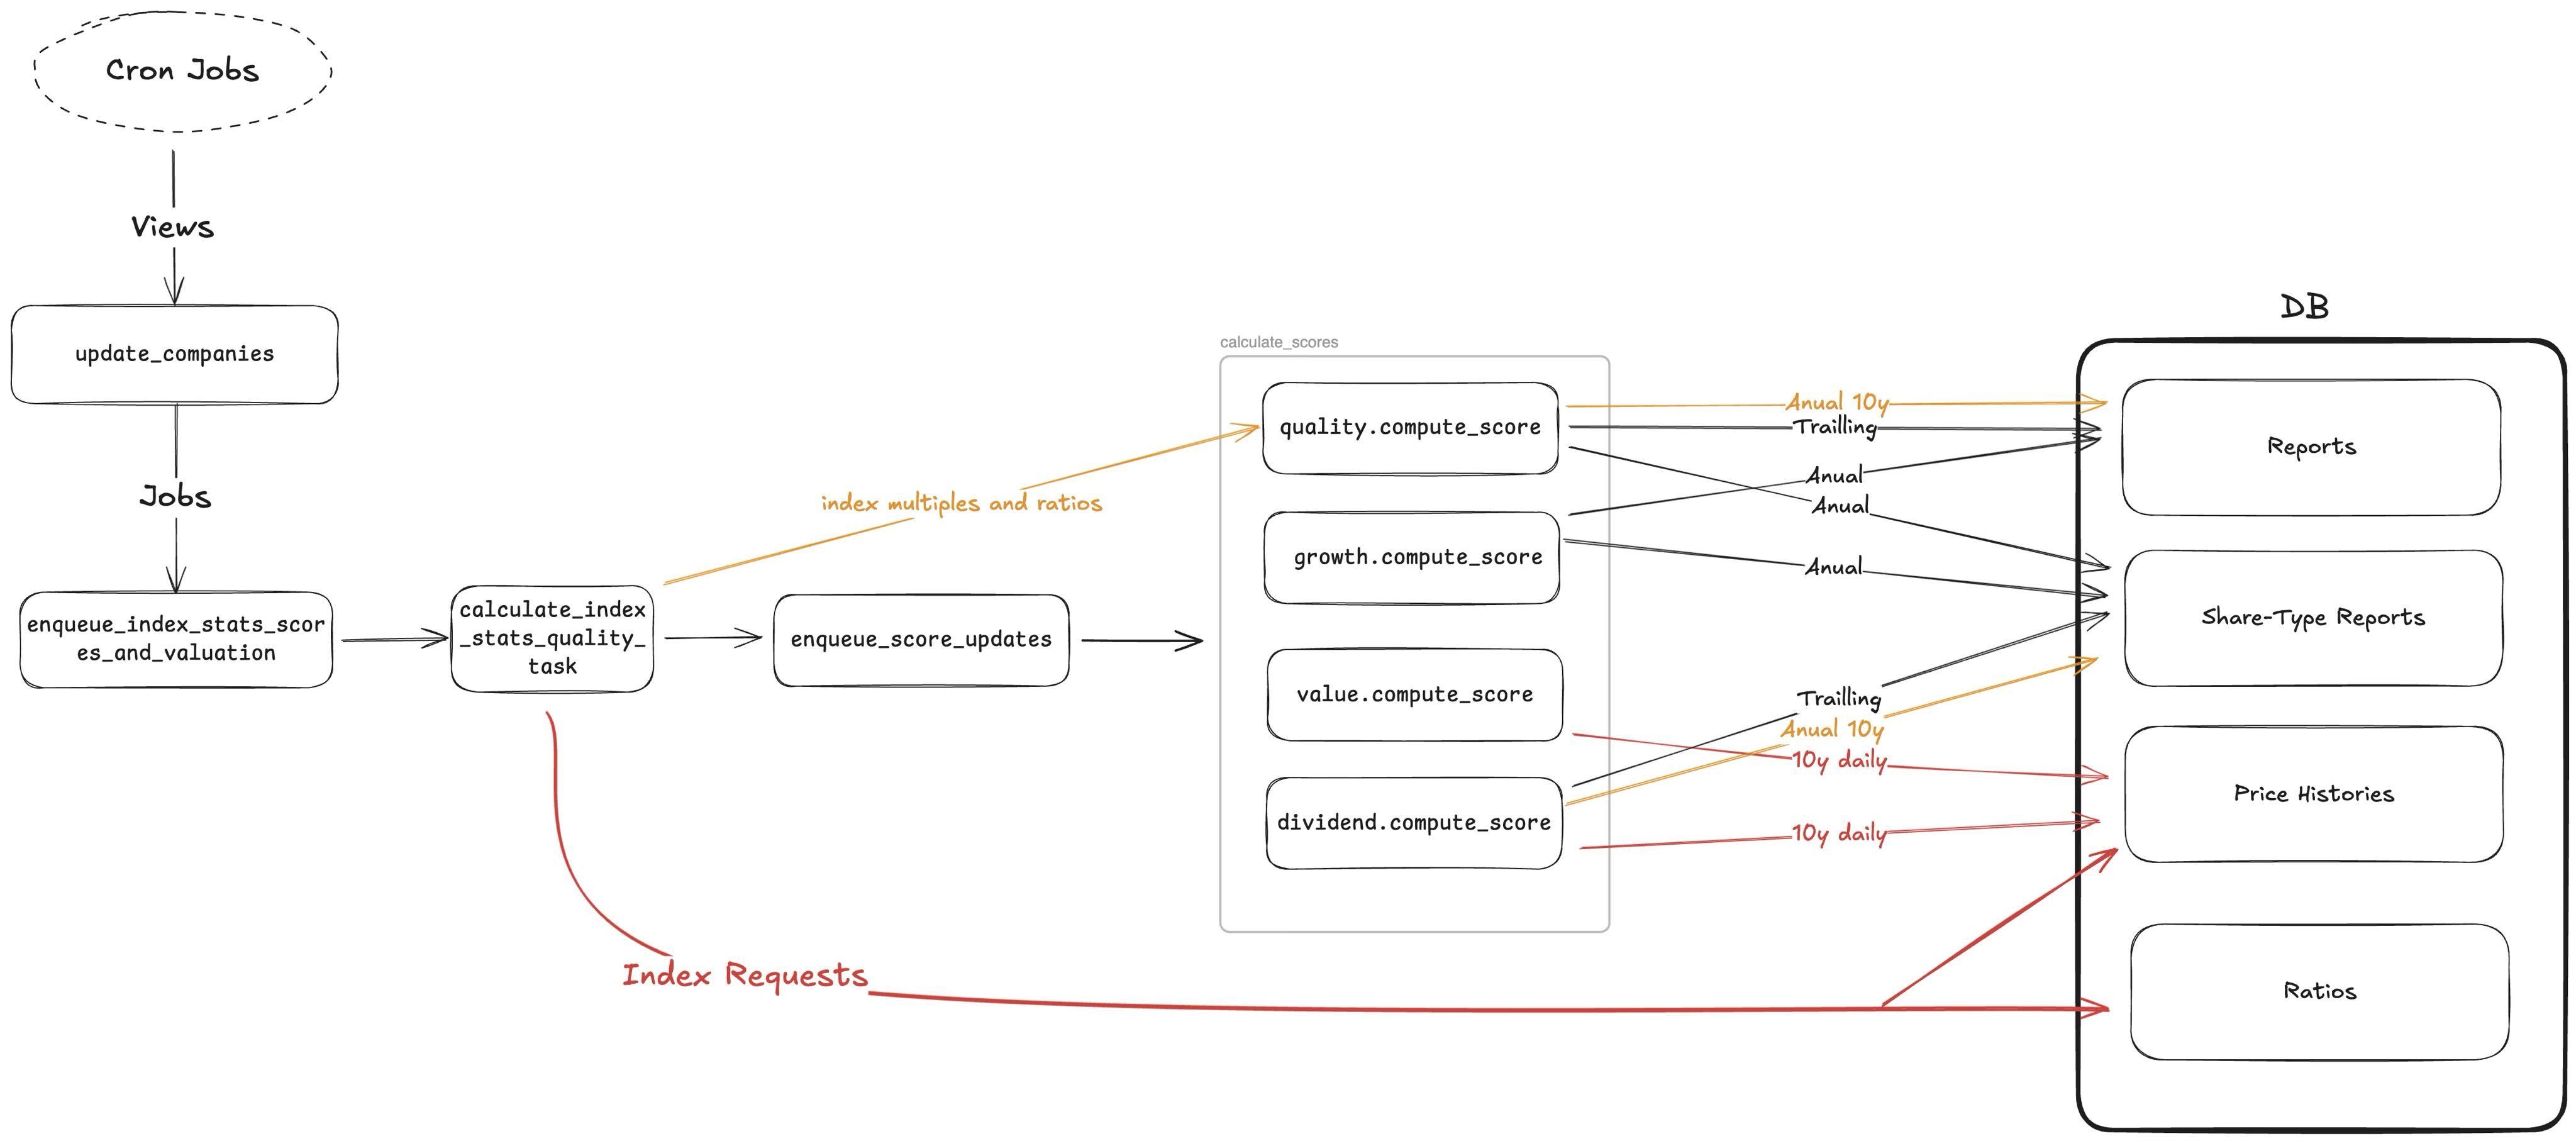
\includegraphics[width=1\textwidth]{images/tweenvest/scores schema.png}
    \caption{Scores Calculations Code Schema}
    \label{fig:scores_schema}
\end{figure}

\noindent With this schema we have simplified the logic behind several functions related to the calculations of each factor score. Quickly we realized that we had to modify the queries to include an extra filter, \textit{calculation\_date} to get the models related to the score at any time, this way we can set it as "today" whenever we are calculating the present scores.


\begin{figure}[H]
    \centering
    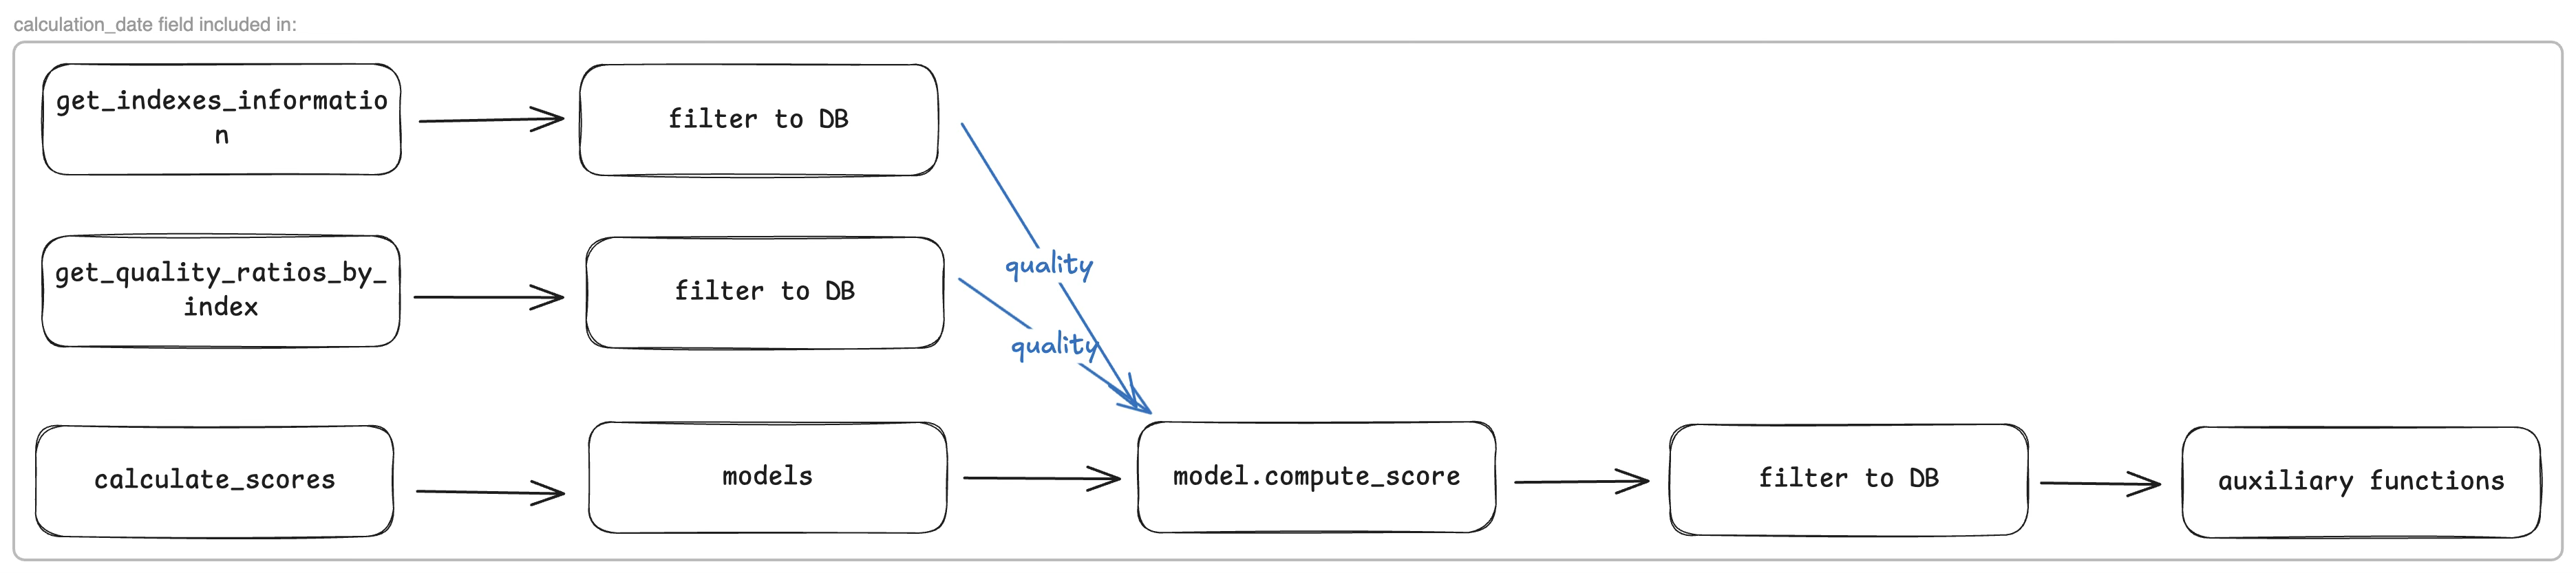
\includegraphics[width=1\textwidth]{images/tweenvest/Propagation Schema.png}
    \caption{\textit{calculation\_date} Field Propagation Schema}
    \label{fig:propagation_schema}
\end{figure}

\vspace{0.5cm}
\noindent Following the propagation schema in Figure \ref{fig:propagation_schema}, the root change comes from the functions \textit{calculate\_scores}, \textit{get\_indexes\_information} and \textit{get\_quality\_ratios\_by\_index}. These are the ones used by the production cron jobs to calculate the factor scores daily, so for a normal function call we set the \textit{calculation\_date} to None and whenever we want to calculate the scores for a specific date we set it to the desired date. 

\vspace{0.5cm}
\noindent This helped us create very readable logic to adapt the filters to both scenarios, for example in the value score shown in Listing \ref{lst:value_score_filtering}:

\begin{lstlisting}[language=Python, caption={Value Score Filtering}, label={lst:value_score_filtering}]
if calculation_date is None:
    calculation_date = date.today()
    filters = {
        "stock": stock,
        "date__gte": calculation_date - relativedelta(years=10),
    }
else:
    filters = {
        "stock": stock,
        "date__gte": calculation_date - relativedelta(years=10),
        "date__lte": calculation_date,
    }
phs = (
    PriceHistory.objects.filter(**filters)
)
\end{lstlisting}

\noindent So as we can observe, the main change for this part of the code was to add a date filter to get only data "lower than or equal" to the \textit{calculation\_date}. This may seem a bad approximation, but it has to be done this way due to the nature of the data: most of the financial data come from annual, semestral, and quarterly reports, except to the price history that is updated daily.

\vspace{0.5cm}
\noindent Along the way of analyzing the code's structure we made some adjustments to simplify the legibility:
\begin{itemize}
    \item \textbf{Renaming functions} whenever they are internal methods or generic auxiliary methods called by different functions.
    \item \textbf{Externalizing mocking functions} that help create fake models and data for unit testing.
    \item \textbf{Homogenize the code's structure}, field types, to help with readability and keeping a standard order along the backend and frontend.
\end{itemize}

\vspace{0.5cm}
\noindent Another very important part of these updating procedure was to \textbf{adapt the unit tests} to make sure that the original code still behaved as expected, and creating new ones to check that the changes calculated the factor scores properly.

\subsection{Designing new Jobs}

Once all tests have passed and the team had approved the changes, the next step was to create scripts —from now on, \textit{jobs}—to populate the current DB with the historic factor scores while maintaining the servers performance in normal levels. For this, we had to update a basic method, \textit{bulk\_create\_or\_update}, used many times through the whole codebase and add a new conditioning so it can handle conflicts depending if the models are empty or not. After reading the official Django \textcite{django2025queryset}, we saw that in newest versions they had included new fields to its original method \textit{bulk\_create}, so we had to update the Django version in our Docker machine and make sure this didn't introduce any unwanted issues.

\vspace{0.5cm}
\noindent After this was implemented, we decided to create three different jobs for enqueueing the tasks and being able to separate the calculations. This way we could restart them in case something broke during the process (see Appendix \ref{app:historical_scores_job}). Also, we had to manage the server resources, so for assuring the platform's performance, we used the following hierarchy (see Listing \ref{lst:lst:tweenvest_production_workers_management}):
\begin{enumerate}
    \item Seven workers for primary daily jobs from different API data integration
    \item One dedicated worker for guaranteeing email sendings, and 6 prioritized shared workers
    \item Four shared workers with lower priority, except for 1 which is set higher than email.
\end{enumerate}

\vspace{0.5cm}
\noindent A crucial part of this code was replicability, equal distribution through different sectors, and mostly to assure that the companies existed during enough time for the factor scores to calculate the 10 years averages.
\begin{figure}[H]
    \centering
    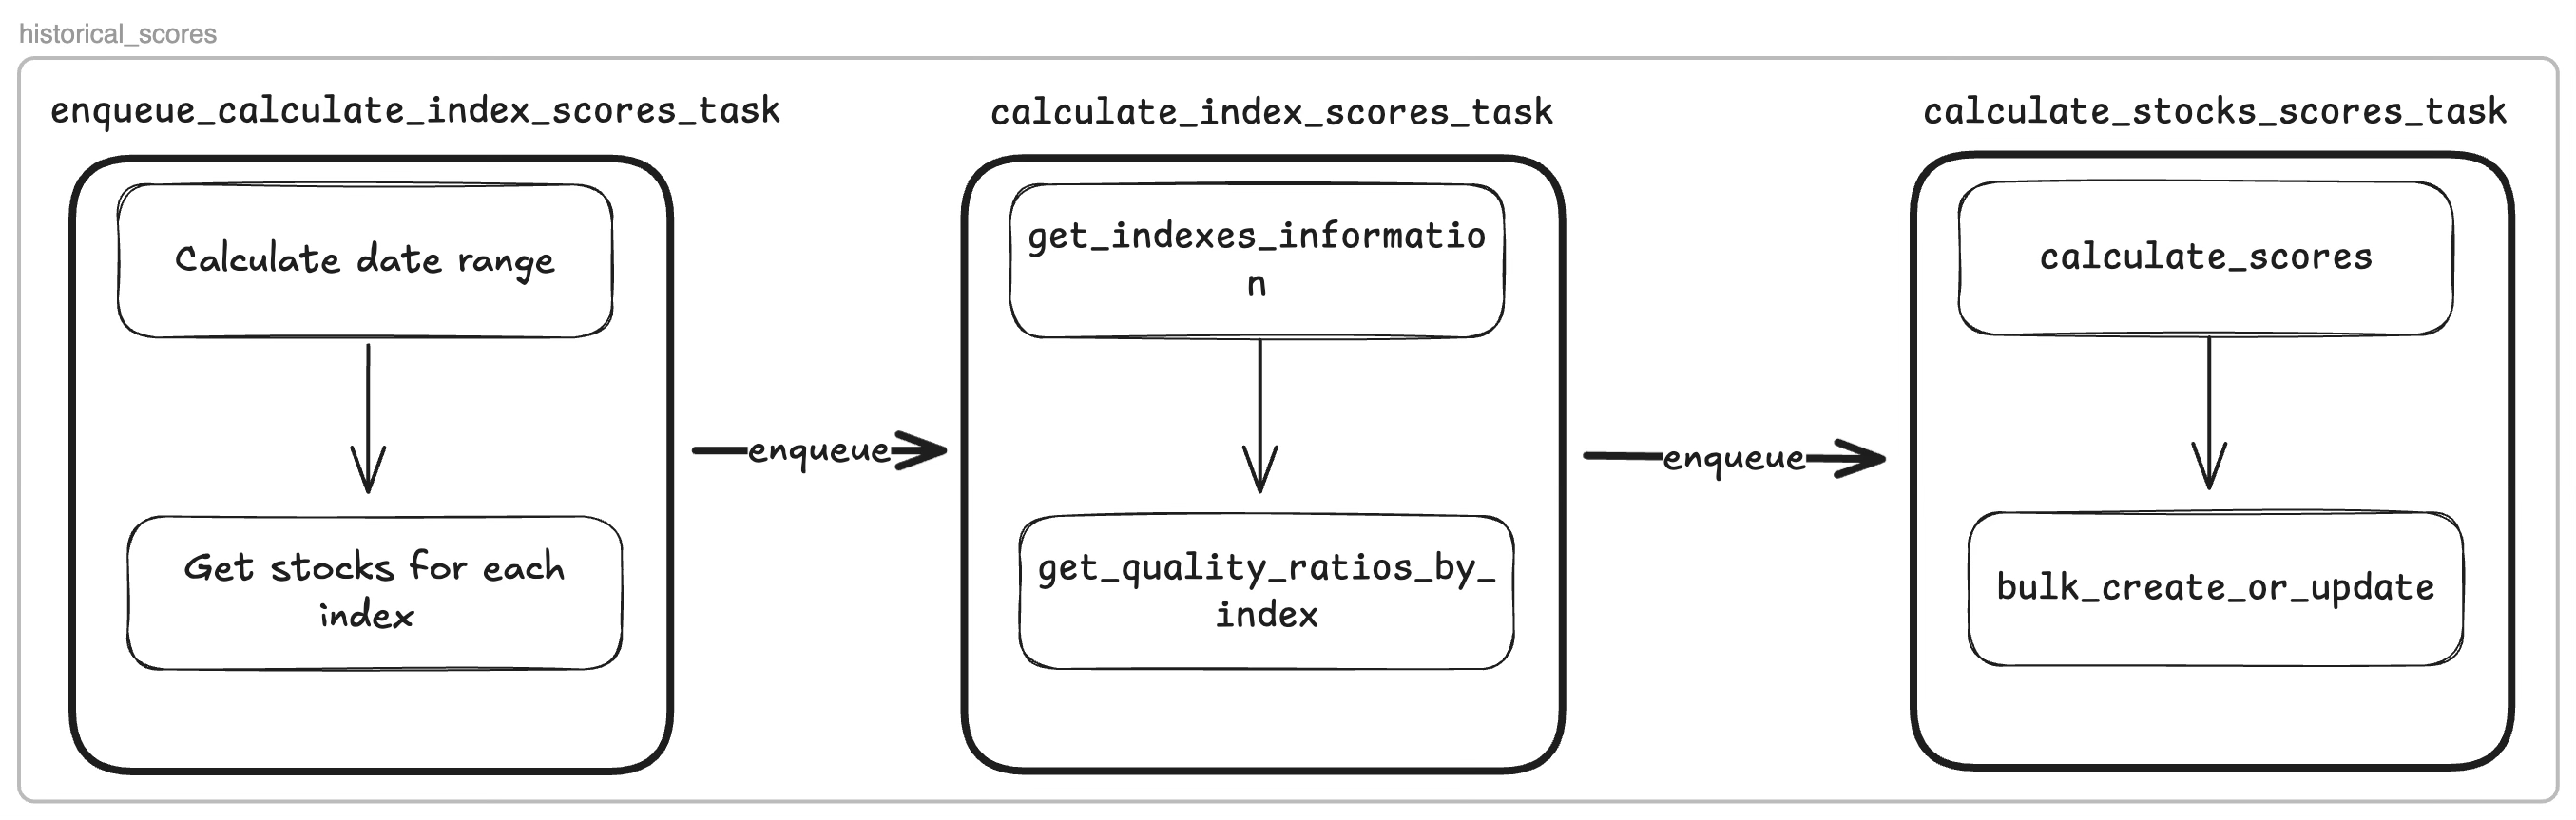
\includegraphics[width=1\textwidth]{images/tweenvest/Historical Jobs First Iteration.png}
    \caption{Historical Jobs First Iteration Schema}
    \label{fig:historical_jobs_first_iteration}
\end{figure}

\noindent We created the first jobs with the schema shown in Figure \ref{fig:historical_jobs_first_iteration}, and during the first small test it worked in local, but when tested with the production DB we started to see important issues with how the functions where designed due to the large amount of data being processed:
\begin{itemize}
    \item Passing incorrect arguments between jobs—such as entire lists of stock objects—led to the REDIS database reaching its maximum storage capacity.
    \item Jobs ran out of time.
\end{itemize}

\begin{figure}[H]
    \centering
    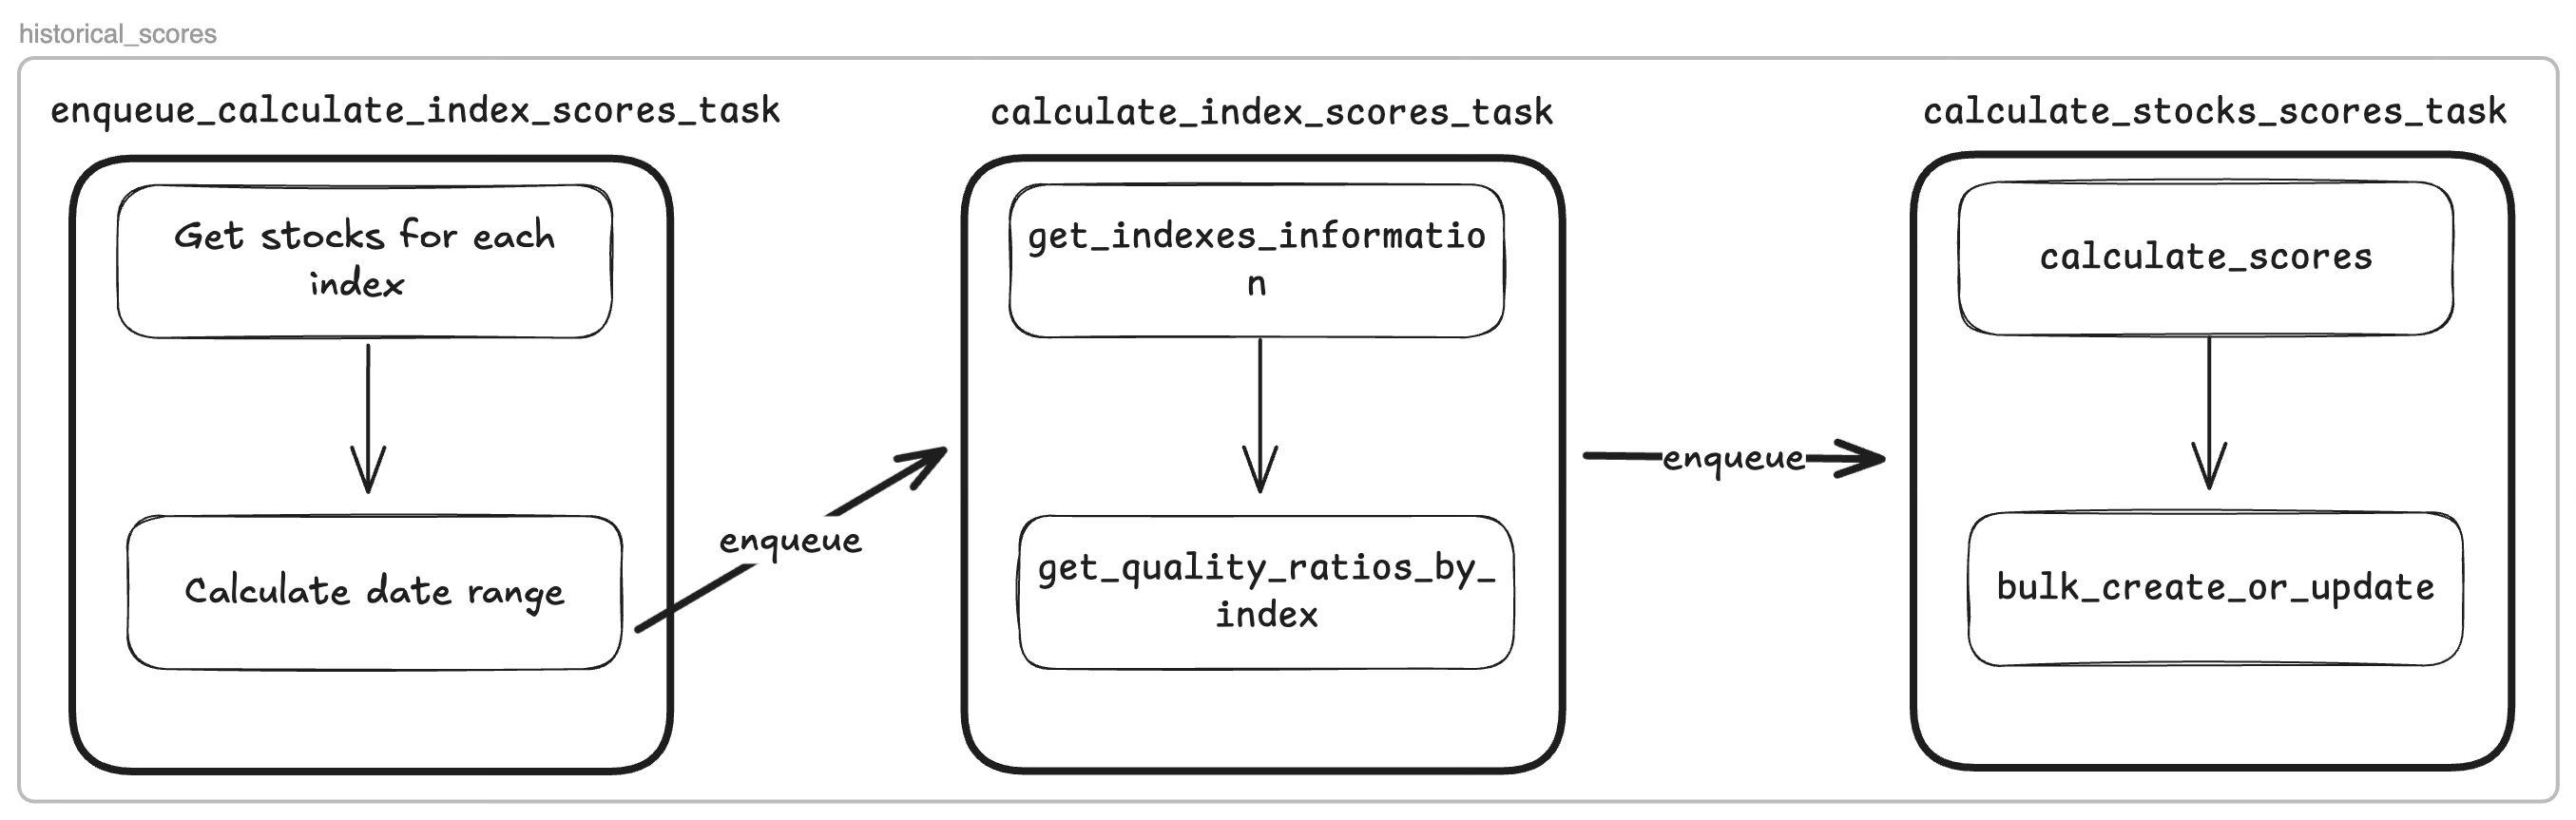
\includegraphics[width=1\textwidth]{images/tweenvest/Historical Jobs Final Version.png}
    \caption{Historical Jobs Final Version Schema}
    \label{fig:historical_jobs_final_version}
\end{figure}

\noindent We then changed the day range logic to enqueue a \textit{calculate\_index\_scores\_task} for each day, so the job didn't have to calculate all of the index data for the dates at all at once, as shown in Figure \ref{fig:historical_jobs_final_version}. Also, we modified the function args to only uses models identifiers "id" to reduce the REDIS memory used. The complete implementation of this job can be found in Appendix \ref{app:historical_scores_job}.

\subsection{Telemetry Tracing}
Finally we had the functional jobs for calculating the scores, and ran the first calculation for a dataset of 1,500 stocks. After the first jobs finished we quickly realized that they were taking too much time to process, and saw a disproportionate amount of queries to the DB so we started a process to check on where was the bottleneck using telemetry tracing tools.

\vspace{0.5cm}
\noindent To do so, we had to inspect each method and function that was being used through the calculations of the factor scores. Luckily we had just recently implemented \textit{DataDog} which is a software that provides monitoring and analytics for applications and infrastructure, offering real-time metrics, event monitoring, and end-to-end tracing.

\vspace{0.5cm}
\noindent To apply the tracer, we simply had to add a specific decorator before each method and set up the environment for being able to trace not only production launched jobs, but also development tests.

\vspace{0.5cm}
\noindent Here's an example of how the tracer was implemented in the quality score calculation:

\begin{lstlisting}[language=Python, caption=Telemetry Tracing Implementation, label={lst:telemetry_tracing_implementation}]
from opentelemetry import trace

tracer = trace.get_tracer(__name__)

@tracer.start_as_current_span("compute_quality_score")
def compute_quality_score(
    stock: "Stock",
    index_quality_ratios: Dict[str, IndexRatio],
    calculation_date: date | None,
) -> tuple[dict, dict]:
    ...
    return final_score
\end{lstlisting}

\noindent We then looked at the \textit{DataDog} dashboard and clearly saw an excess of queries to the DB when calculating each score, and tried to reduce them by looking for a simple fault in the logic of the queries. Similar issues had been resolved before by adding a \textit{select\_related} in the queries. To clarify what this does, here is the definition with a simple use-case:

\vspace{0.5cm}
\noindent ``Returns a QuerySet that will follow foreign-key relationships, selecting additional related-object data when it executes its query. This is a performance booster which results in a single more complex query but means later use of foreign-key relationships won't require database queries.'' -- \textcite{django2025selectrelated}.

\vspace{0.5cm}
\noindent In Django, \textit{select\_related()} and \textit{prefetch\_related()} are designed to stop the deluge of database queries that are caused by accessing related objects. \textit{select\_related()} ``follows'' foreign-key relationships, selecting additional related-object data when it executes its query. \textit{prefetch\_related()} does a separate lookup for each relationship and does the ``joining'' in Python. So one uses \textit{select\_related} when the object that you're going to be selecting is a single object, so \textit{OneToOneField} or a \textit{ForeignKey}.

\vspace{0.5cm}
\noindent After numerous attempts to improve performance, we were forced to reconsider our approach and began analyzing the problem from a different perspective. It quickly became evident that we were operating on a small virtual machine (Table~\ref{tab:tweenvest_server_specs}) shared with the regular platform workload. Tweenvest’s servers are not designed for high computational demand; rather, they are optimized for routine operations, where standard score calculations typically take between 3 to 4 hours. This setup works well under normal conditions, as calculations are performed after market hours and do not impact the user experience. However, it proved inadequate for our needs—specifically, processing data over five or more years within a reasonable timeframe, even when computing just one score per month.

\begin{table}[H]
    \centering
    \begin{tabular}{|l|l|l|l|}
        \hline
        \textbf{VCPUS} & \textbf{RAM} & \textbf{SSD Storage} & \textbf{Extra Volume} \\
        \hline
        8 & 4 GB & 320 GB & -- \\
        \hline
    \end{tabular}
    \caption{Tweenvest Server Specifications}
    \label{tab:tweenvest_server_specs}
\end{table}


\subsection{Dedicated Server Deployment}
\noindent We made the decision to establish a dedicated server for this thesis, equipped with enhanced computational power to facilitate the calculations and data fitting.After evaluating several providers, we opted for Hetzner servers due to their exceptional quality-price ratio. The final setup consists of a dedicated server with the following specifications:

\begin{table}[H]
    \centering
    \begin{tabular}{|l|l|l|l|l|l|}
        \hline
        \textbf{VCPUS} & \textbf{RAM} & \textbf{SSD Storage} & \textbf{Extra Volume} \\
        \hline
        16 & 32 GB & 320 GB & 480 GB \\
        \hline
    \end{tabular}
    \caption{Hetzner Server Specifications}
    \label{tab:hetzner_server_specs}
\end{table}

\noindent Deploying the project in a scalable and reproducible environment involved several structured steps, encompassing server provisioning, secure remote access configuration using SSH, and initializing the containerized application deployment via Docker, with the application codebase managed through GitHub.

\vspace{0.5cm}  
\noindent After all of the setup was done, we saw an amazing \textbf{x100 performance improvement}, going from 15-minute calculation times for index statistics to 8 seconds. Finally, we could launch the factor scores historical calculations, so we created two subsets of 1,500 random companies each with the factor scores calculated for the 1st day of the month for the following periods: 2015-2020 and 2020-2025, which took a total of 3 hours.

\vspace{0.5cm}
\noindent Now that we had filled the DB with the necessary factor scores for the study, we ran a big calculation to get all of the possible factor scores for the +100,000 companies, which took several days.

\section{Dataset Creation}

\subsection{Aggregating the data}

For being able to continue, we needed to create the final dataset with all the necessary data for later on doing the analysis and developing the predictive models, so we created a simple algorithm with this logic:

\begin{figure}[H]
    \centering
    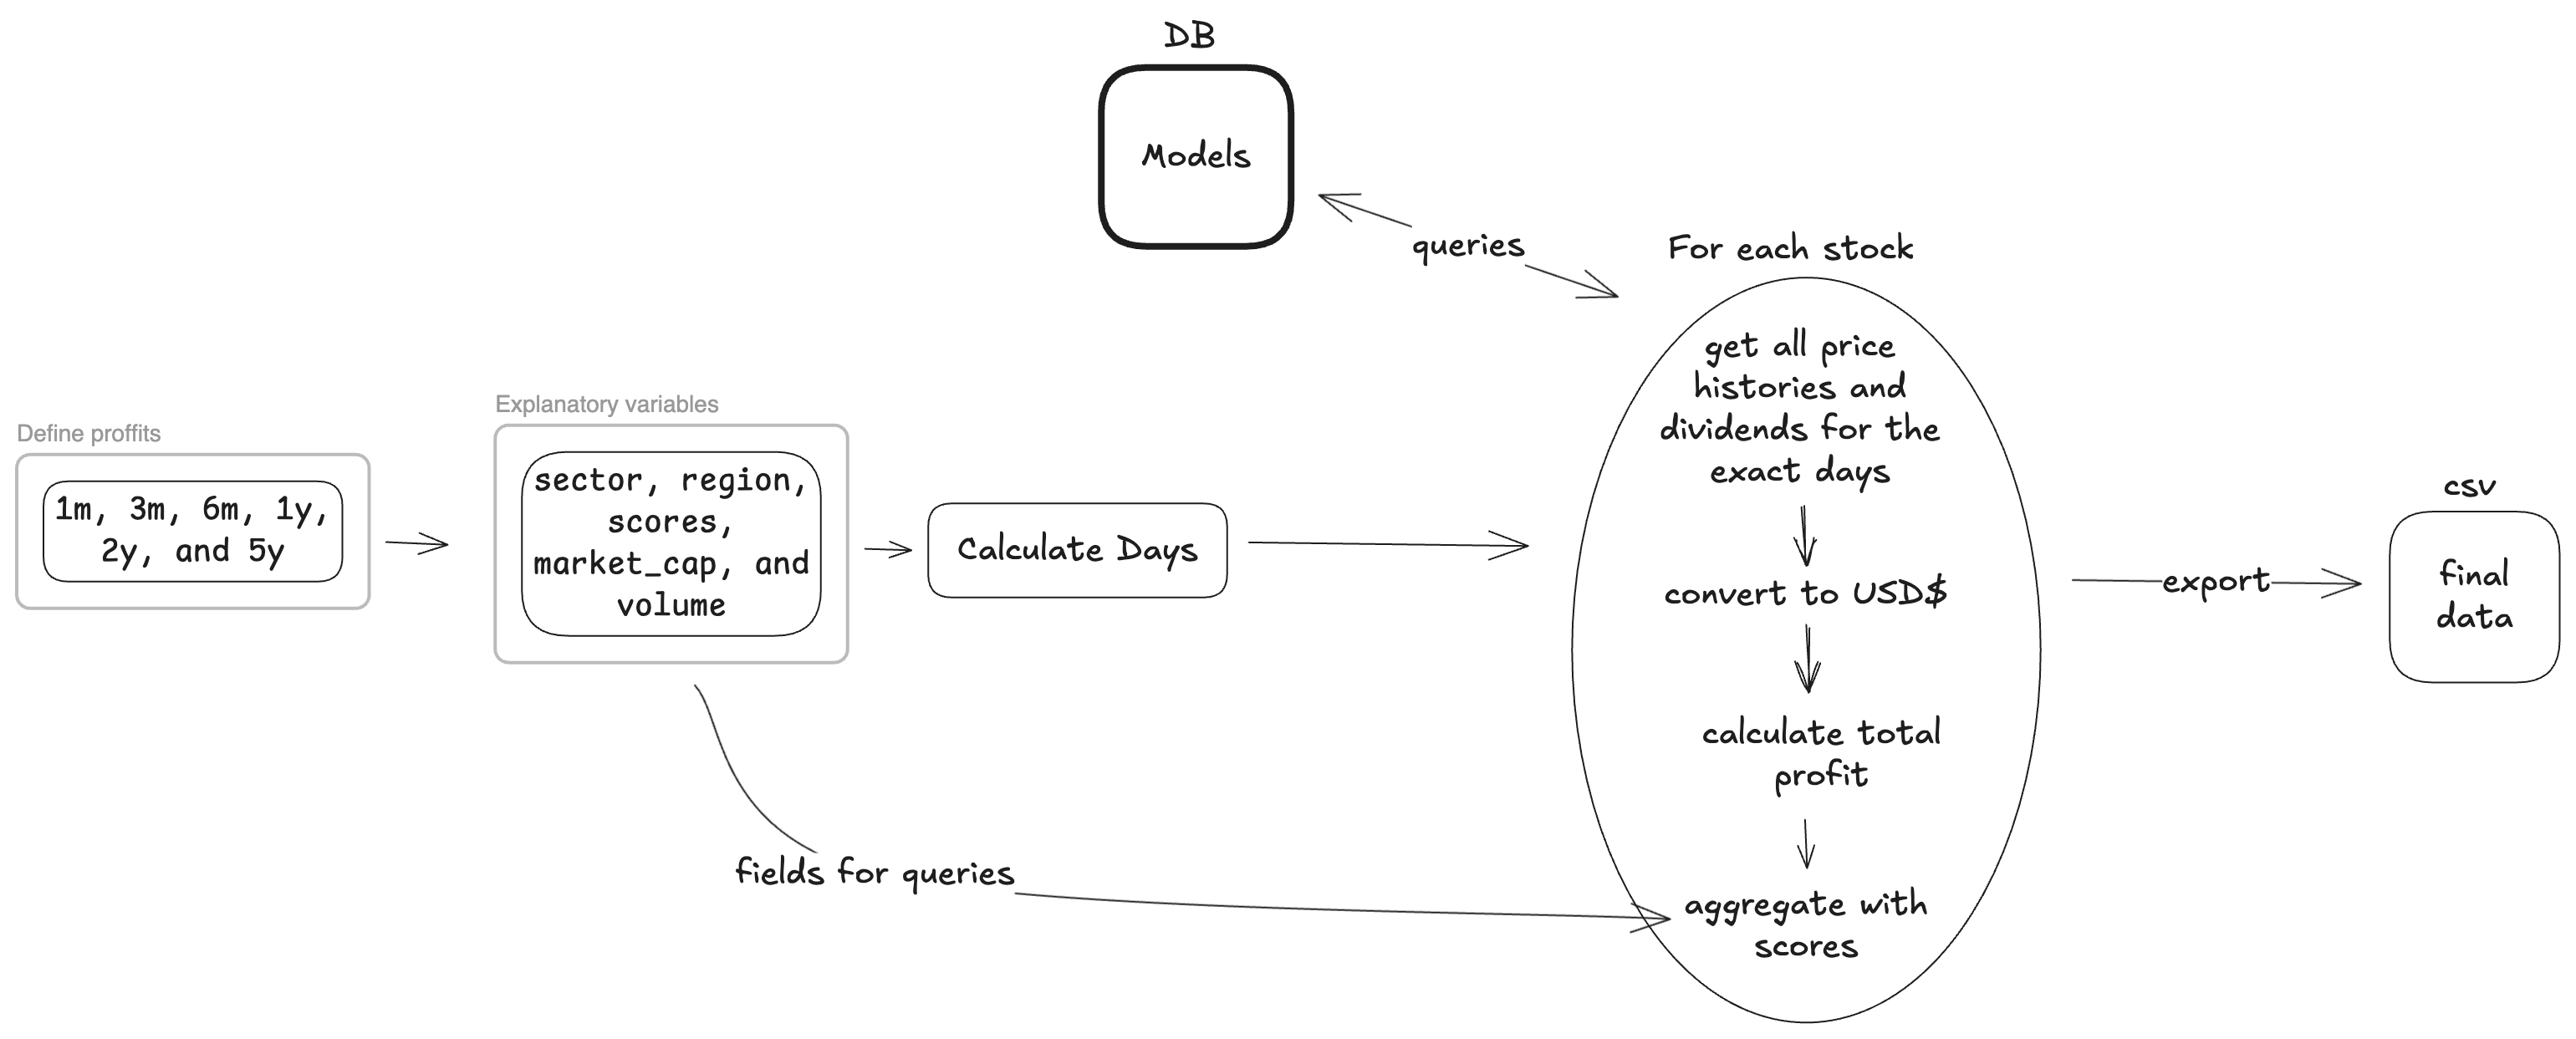
\includegraphics[width=0.8\textwidth]{images/tweenvest/First Data Aggregation Schema.png}
    \caption{First Data Aggregation Schema}
    \label{fig:first_data_aggregation_schema}
\end{figure}

\noindent Once we had the final csv file we noticed that we had too many empty values for profits, the problem was because some of the days calculated were empty for a specific company, so there was no price history for them. Since the companies belong to multiple countries, the different holidays could be causing another major loss in the information. To fix this in a general way we implemented an internal method for estimating price histories if they didn't exist for the wanted date. The complete implementation of this data export and price estimation process can be found in Appendix \ref{app:data_export_job}.

\begin{figure}[H]
    \centering
    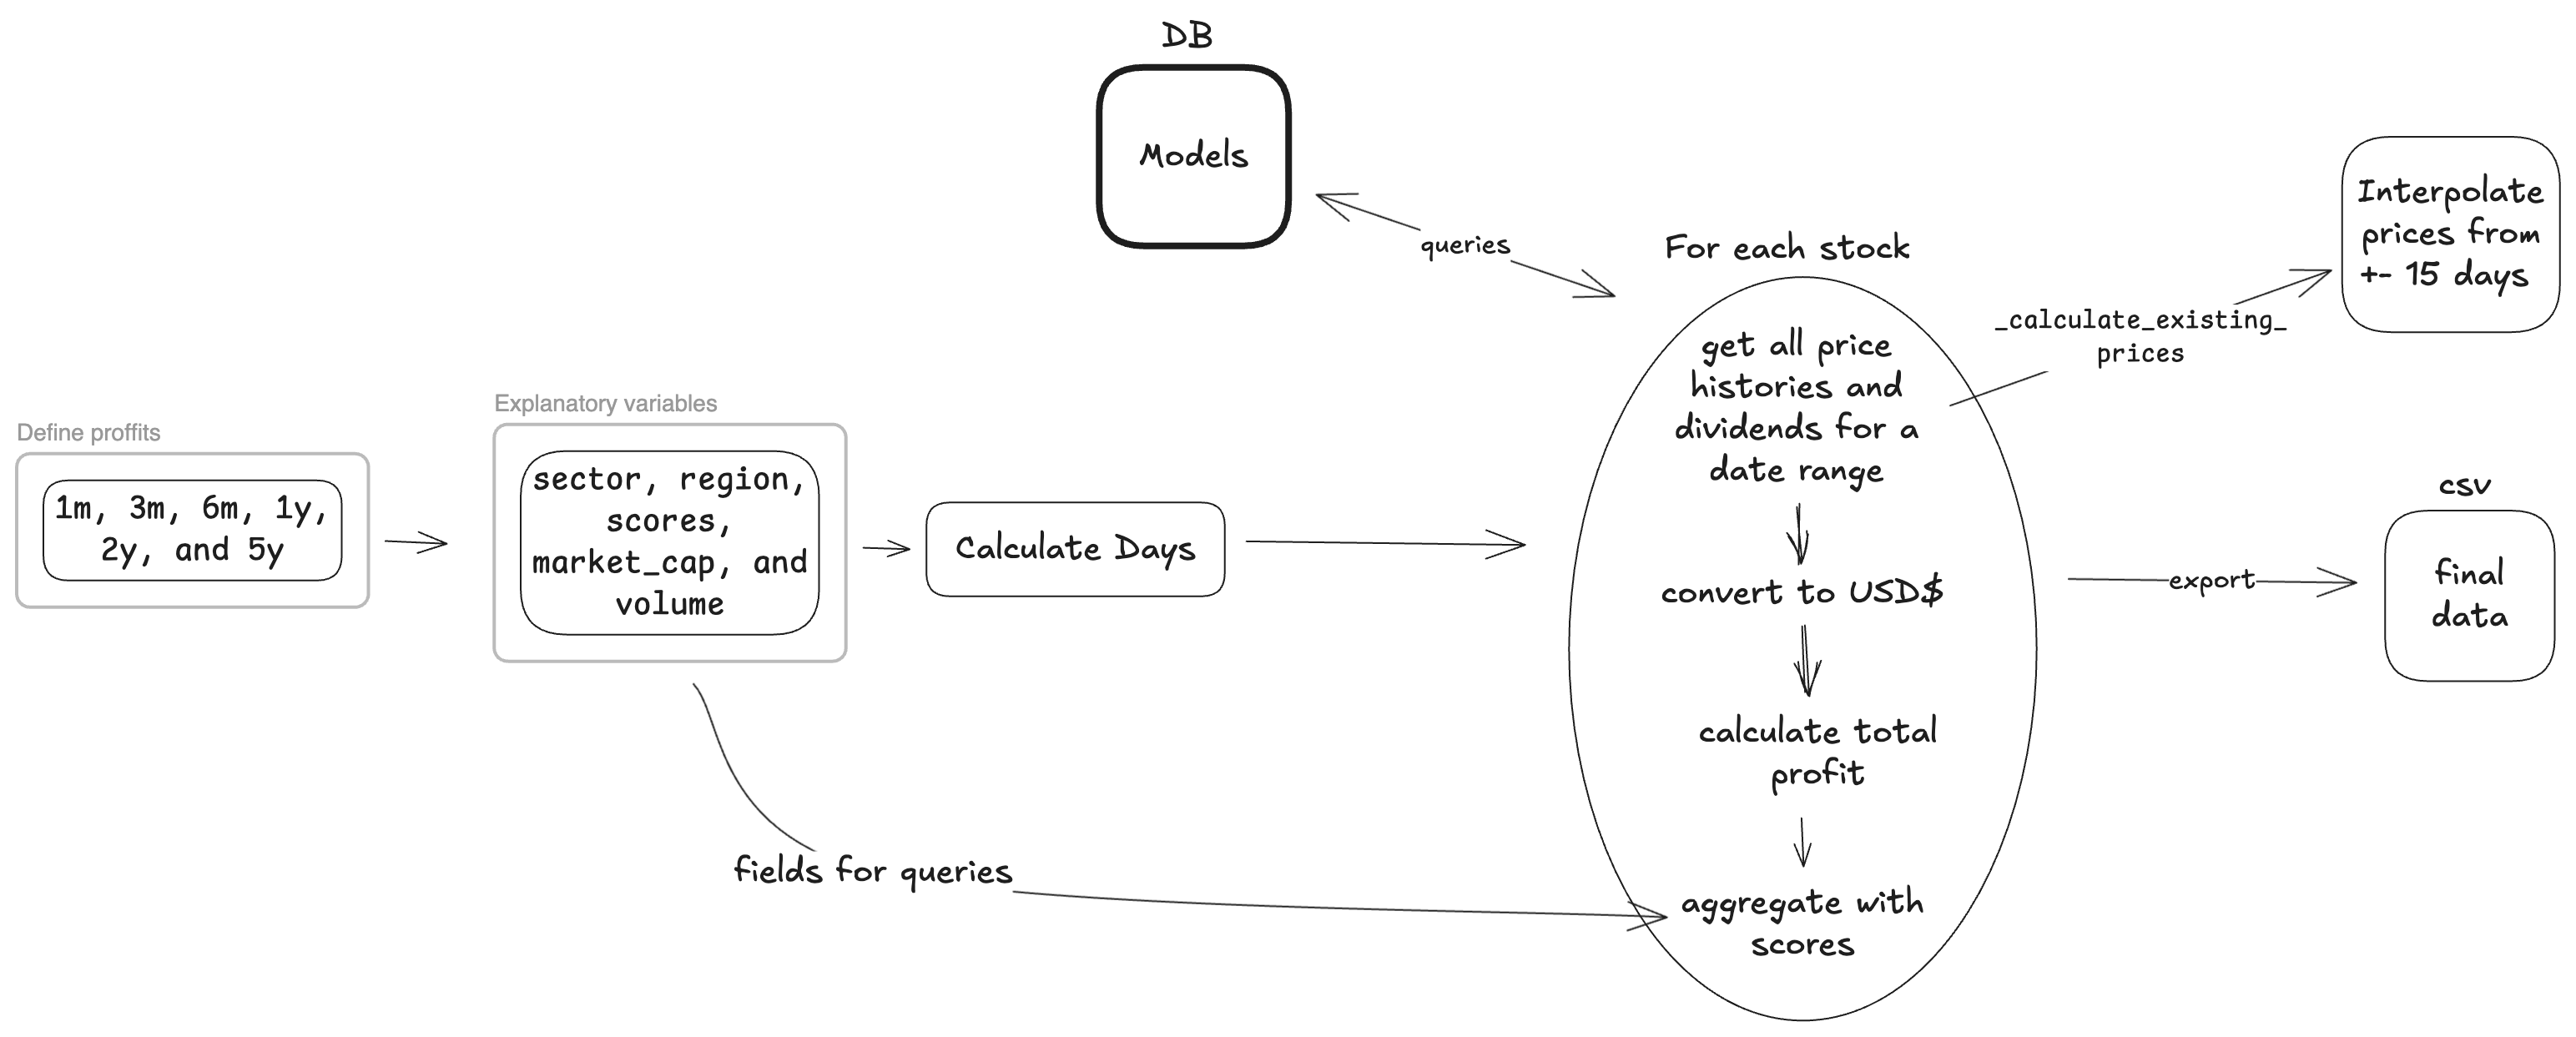
\includegraphics[width=0.8\textwidth]{images/tweenvest/Final Data Aggregation Schema.png}
    \caption{Final Data Aggregation Schema}
    \label{fig:final_data_aggregation_schema}
\end{figure}

\noindent This can be done due to the fact that we are only looking for long term profitabilities, so we can \textbf{approximate the price} on a day $x$ by interpolating the price on $x-y$ and $x+z$, weighted by how close they are to the original day $x$, with a maximum distance from $x$ of 15 days. This significantly reduced the amount of missing values.

\subsection{Datasets Construction}

For this study, we have attacked the main objective from multiple perspectives. First we made a descriptive analysis to understand the data, and then we proposed different models to see if there were any relationships between the scores factors and long term profitabilities. Thats why when creating the datasets, we made two different approaches to have more information for the analysis:

\begin{figure}[H]
    \begin{minipage}{0.48\textwidth}
        \centering
        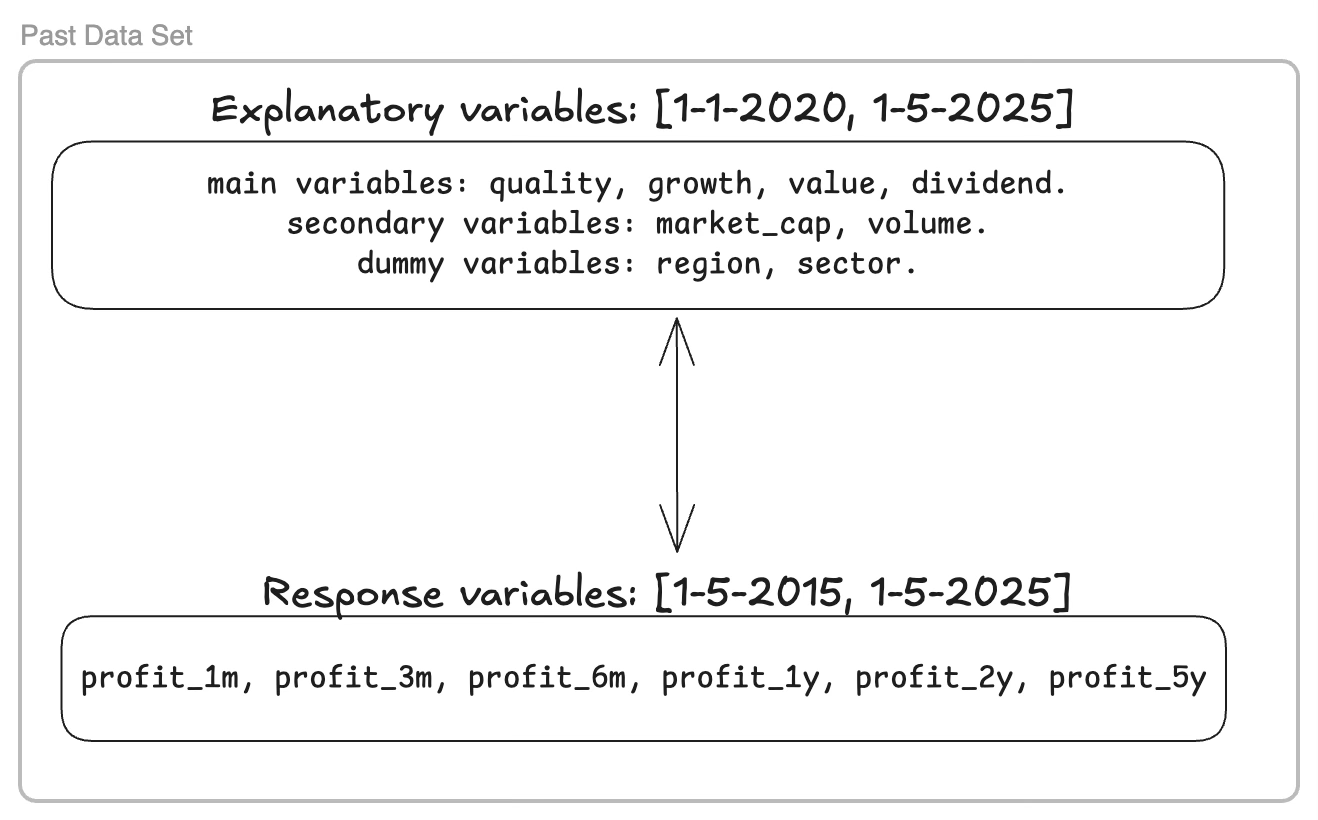
\includegraphics[width=\textwidth]{images/tweenvest/Past Dataset variables relations.png}
        \caption{Past Dataset}
        \label{fig:past_dataset}
    \end{minipage}
    \hfill
    \begin{minipage}{0.48\textwidth}
        \centering
        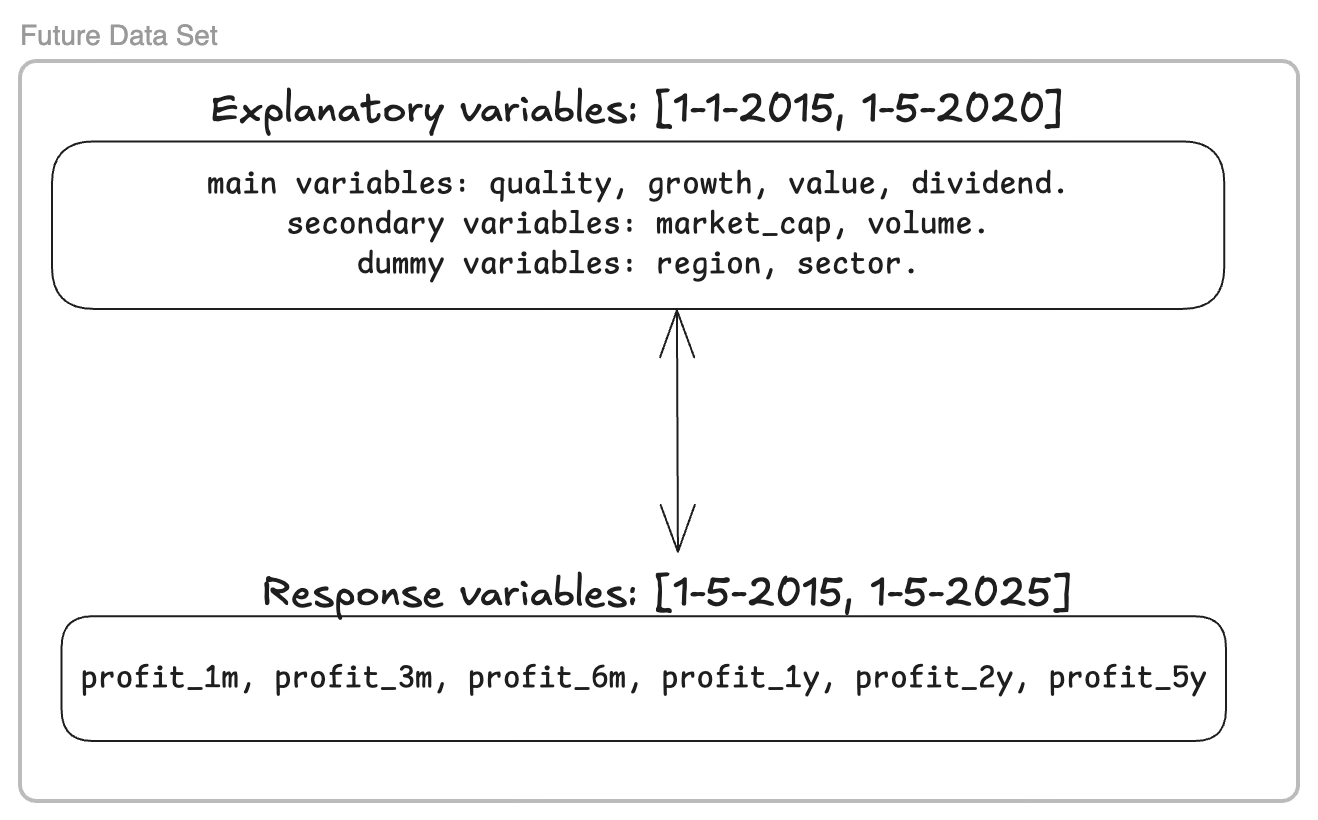
\includegraphics[width=\textwidth]{images/tweenvest/Future Dataset variables relations.png}
        \caption{Future Dataset}
        \label{fig:future_dataset}
    \end{minipage}
\end{figure}

\noindent For the past dataset, we calculated the scores for the range 2020-2025 and then related them to the profits obtained until the specified date. For example, the date 1-1-2021 would be linked to the 2 years' profitability obtained until that date: 
\begin{equation}
    Profit_{1\text{-}1\text{-}2021}(\%) = \frac{P_{1\text{-}1\text{-}2021} - P_{1\text{-}1\text{-}2019} + D_{\text{acc}}}{P_{1\text{-}1\text{-}2019}}
\end{equation}

\noindent Which interprets to \textbf{how earlier profits have influenced on the explanatory variables}. This will give us valuable information in the descriptive analysis.

\vspace{0.5cm}
\noindent For the model fitting, \textbf{we want to know if the current scores are good predictors of the future profits}. So we calculated the scores for the range 2015-2020 and related them to the profits obtained from that date to the future. For example, the date 1-1-2021 would be linked to the 2 years' profitability that will be obtained in the future: 

\begin{equation}
    Profit_{1\text{-}1\text{-}2021}(\%) = \frac{P_{1\text{-}1\text{-}2023} - P_{1\text{-}1\text{-}2021} + D_{\text{acc}}}{P_{1\text{-}1\text{-}2021}}
\end{equation}

\noindent As this approach is what we actually want to use for the predictive models, we will be using the future dataset structure for most of the analysis.

\subsection{Preprocessing}
Even with all of these protocols to create the most reliable and filled datasets, we still had to follow the methodologies explained in the previous chapter to analyze the data.

\subsubsection{Cleaning the Data}
To begin, we looked at the data structure and saw that \textbf{about 50\% of growth scores were empty}. This turned on many alerts from problems with the scores calculation algorithm, because compared to the rest of the variables there was a significant difference, since the \textbf{normal absence was only around 8\%} taking into account the value score as reference because it doesn't have 10 year averages.
\begin{table}[H]
    \centering
    \begin{tabular}{|c|c|c|c|c|c|c|c|c|}
        \hline
        \textbf{quality} & \textbf{growth} & \textbf{value} & \textbf{profit\_1m} & \textbf{profit\_3m} & \textbf{profit\_6m} & \textbf{profit\_1y} & \textbf{profit\_2y} & \textbf{profit\_5y} \\
        \hline
        13.4 & 54.0 & 7.4 & 2.6 & 3.1 & 3.2 & 3.2 & 3.3 & 6.0 \\
        \hline
    \end{tabular}
    \caption{Missing values (\% ) per column for Small Data Future.}
    \label{tab:missing_values_small_data_future}
\end{table}


\noindent   But after digging into the data we saw that it was due to the fact that many companies stopped sending reports or selling but kept existing, so we decided to deleted them from our dataset because they weren't behaving as a "normal company", and this could create a bias in the models. Additionally, as noted earlier, we replaced all NaN values in the dividend scores with 0, since Tweenvest's algorithm omits a score when a company does not pay dividends. That's why we don't see any missing values in the dividend scores.

\vspace{0.5cm}
\noindent This pattern is constant in all of the different datasets, as we can see in this summary table:

\begin{table}[H]
    \centering
    \begin{tabular}{|l|l|l|l|}
        \hline  
        \textbf{Dataset} & \textbf{Raw} & \textbf{Cleaned} & \textbf{No Outliers} \\
        \hline
        \textbf{Big Data Past$^\dagger$} & 16,119,852 & 9,991,895 & 9,492,300 \\
        \hline
        \textbf{Big Data Future$^\dagger$} & 31,933,137 & 14,518,624 & 13,792,692 \\
        \hline 
        \textbf{Small Data Past} & 83,243 & 48,338 & 46,415 \\
        \hline
        \textbf{Small Data Future} & 65,166 & 26,214 & 25,220 \\
        \hline
        \textbf{Small Data Future USA} & 60,503 & 21,240 & 20,463 \\
        \hline
        \textbf{Small Data Future EU} & 62,725 & 25,217 & 24,245 \\
        \hline        
        \textbf{Small Data Future AS} & 65,772 & 28,085 & 27,156\\
        \hline
        \textbf{Small Data Future LAT} & 48,412 & 20,610 & 19,851 \\
        \hline
        \textbf{Small Data Future AF} & 58,341 & 21,182 & 20,335 \\
        \hline
        \end{tabular}

    \caption{Rows per Dataset}
    \label{tab:datasets_summary}
\end{table}

\noindent $^\dagger$ In the \textit{Big Data Past} and \textit{Big Data Future} datasets, we removed the outliers using the Isolation Forest method for saving computational time.


\chapter{Results}
\section{Descriptive Analysis}

Before jumping into the model fitting, it is necessary to understand the data that we are working with.

\subsection{Variables Distributions}

\subsubsection{Scores}
Following the scores order, quality's distribution show a \textbf{clear negative skewness}, meaning that there are more companies closer to having a good quality score. This could be due to the fact that we have deleted companies that don't behave as a "normal company", so we will analize the distributions of the profits to see if there is a bias in the data. Also, there is a \textbf{secondary peak arounf the 30-40 scores}, which could be related to the time-frame of the data.

\begin{figure}[H]
    \centering
    \begin{minipage}{0.48\textwidth}
        \centering
        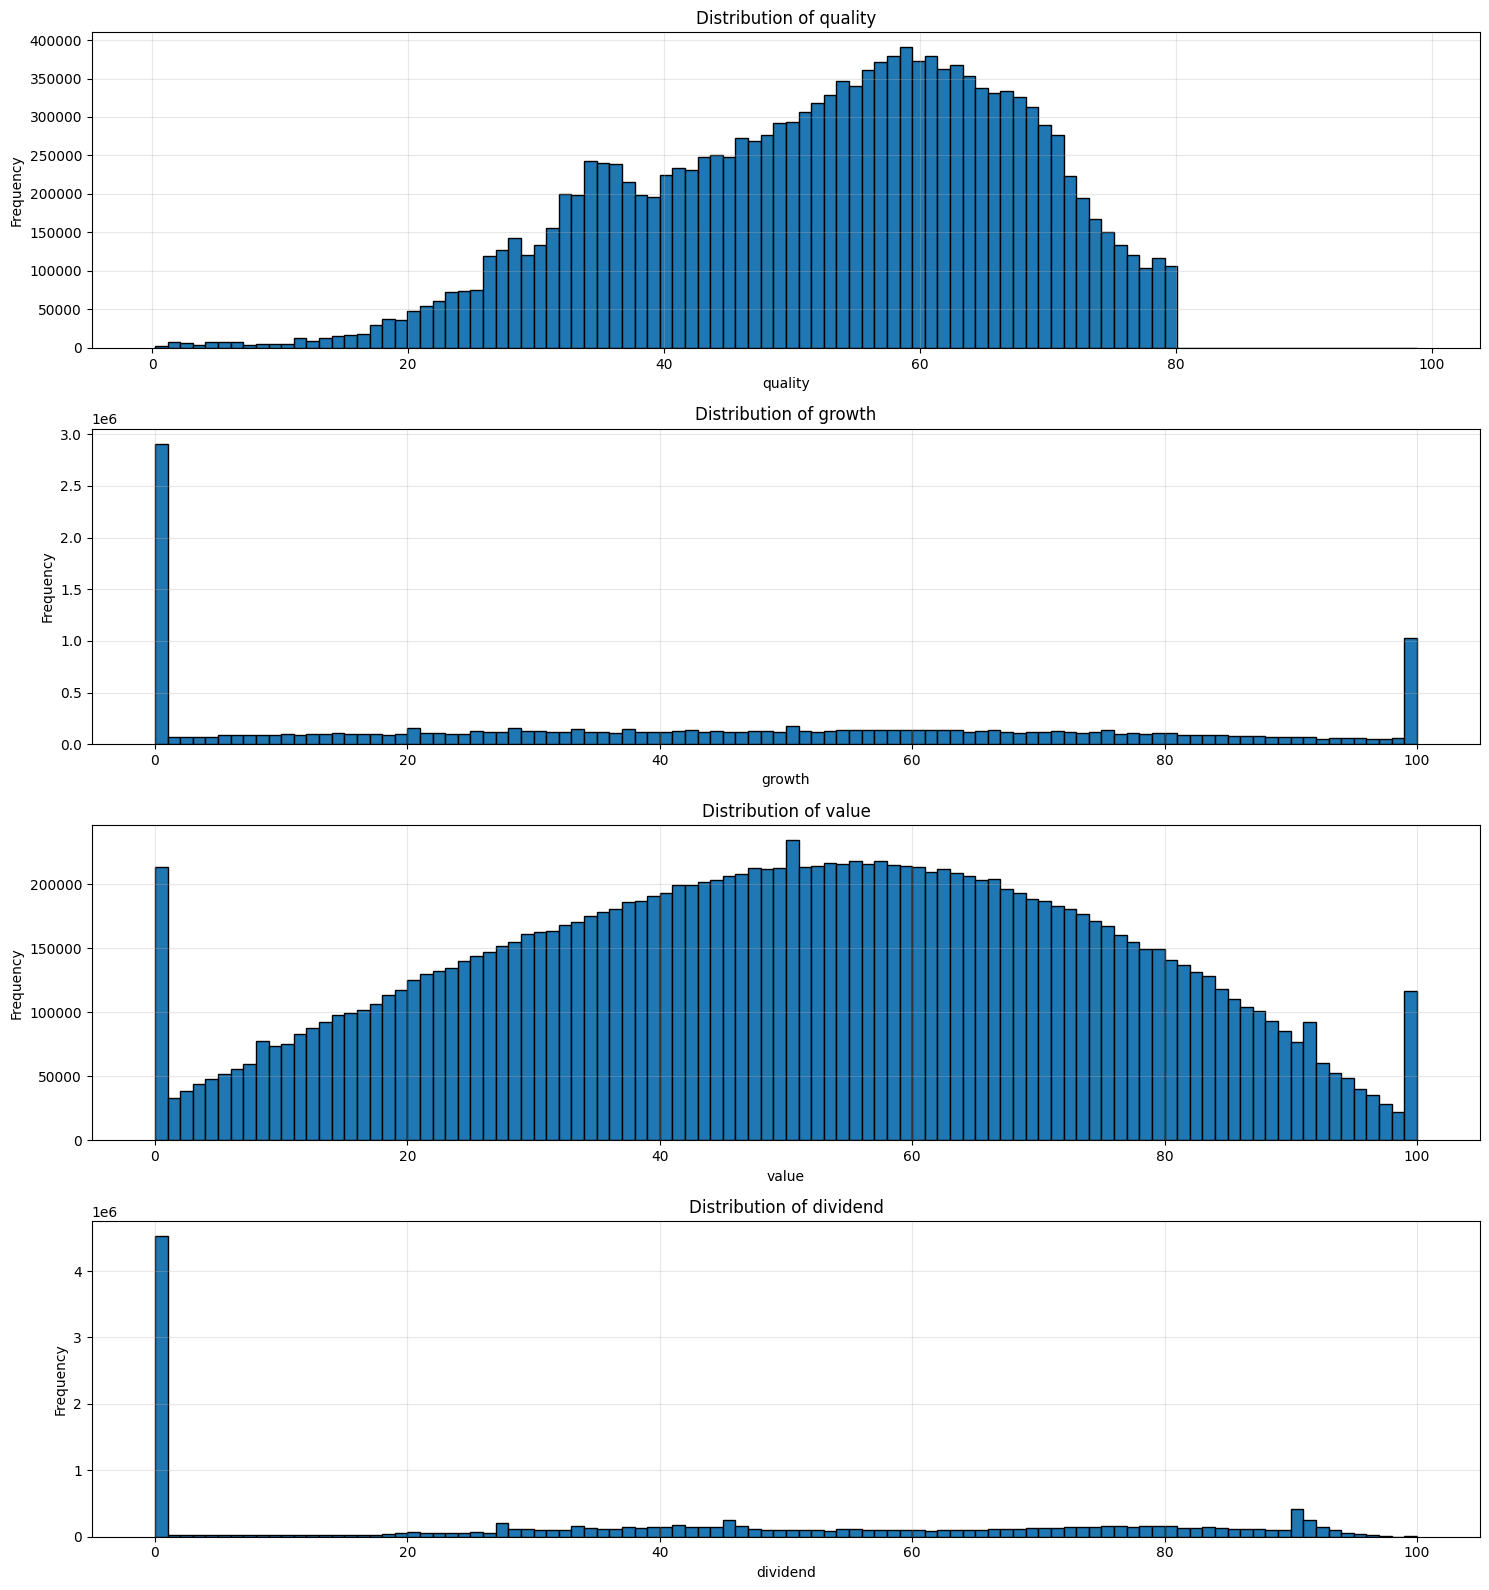
\includegraphics[width=\linewidth]{images/code/descriptive analysis/distributions/Big Data future - Scores.png}
        \caption{Big Data Future - Scores}
        \label{fig:scores}
    \end{minipage}\hfill
    \begin{minipage}{0.48\textwidth}
        \centering
        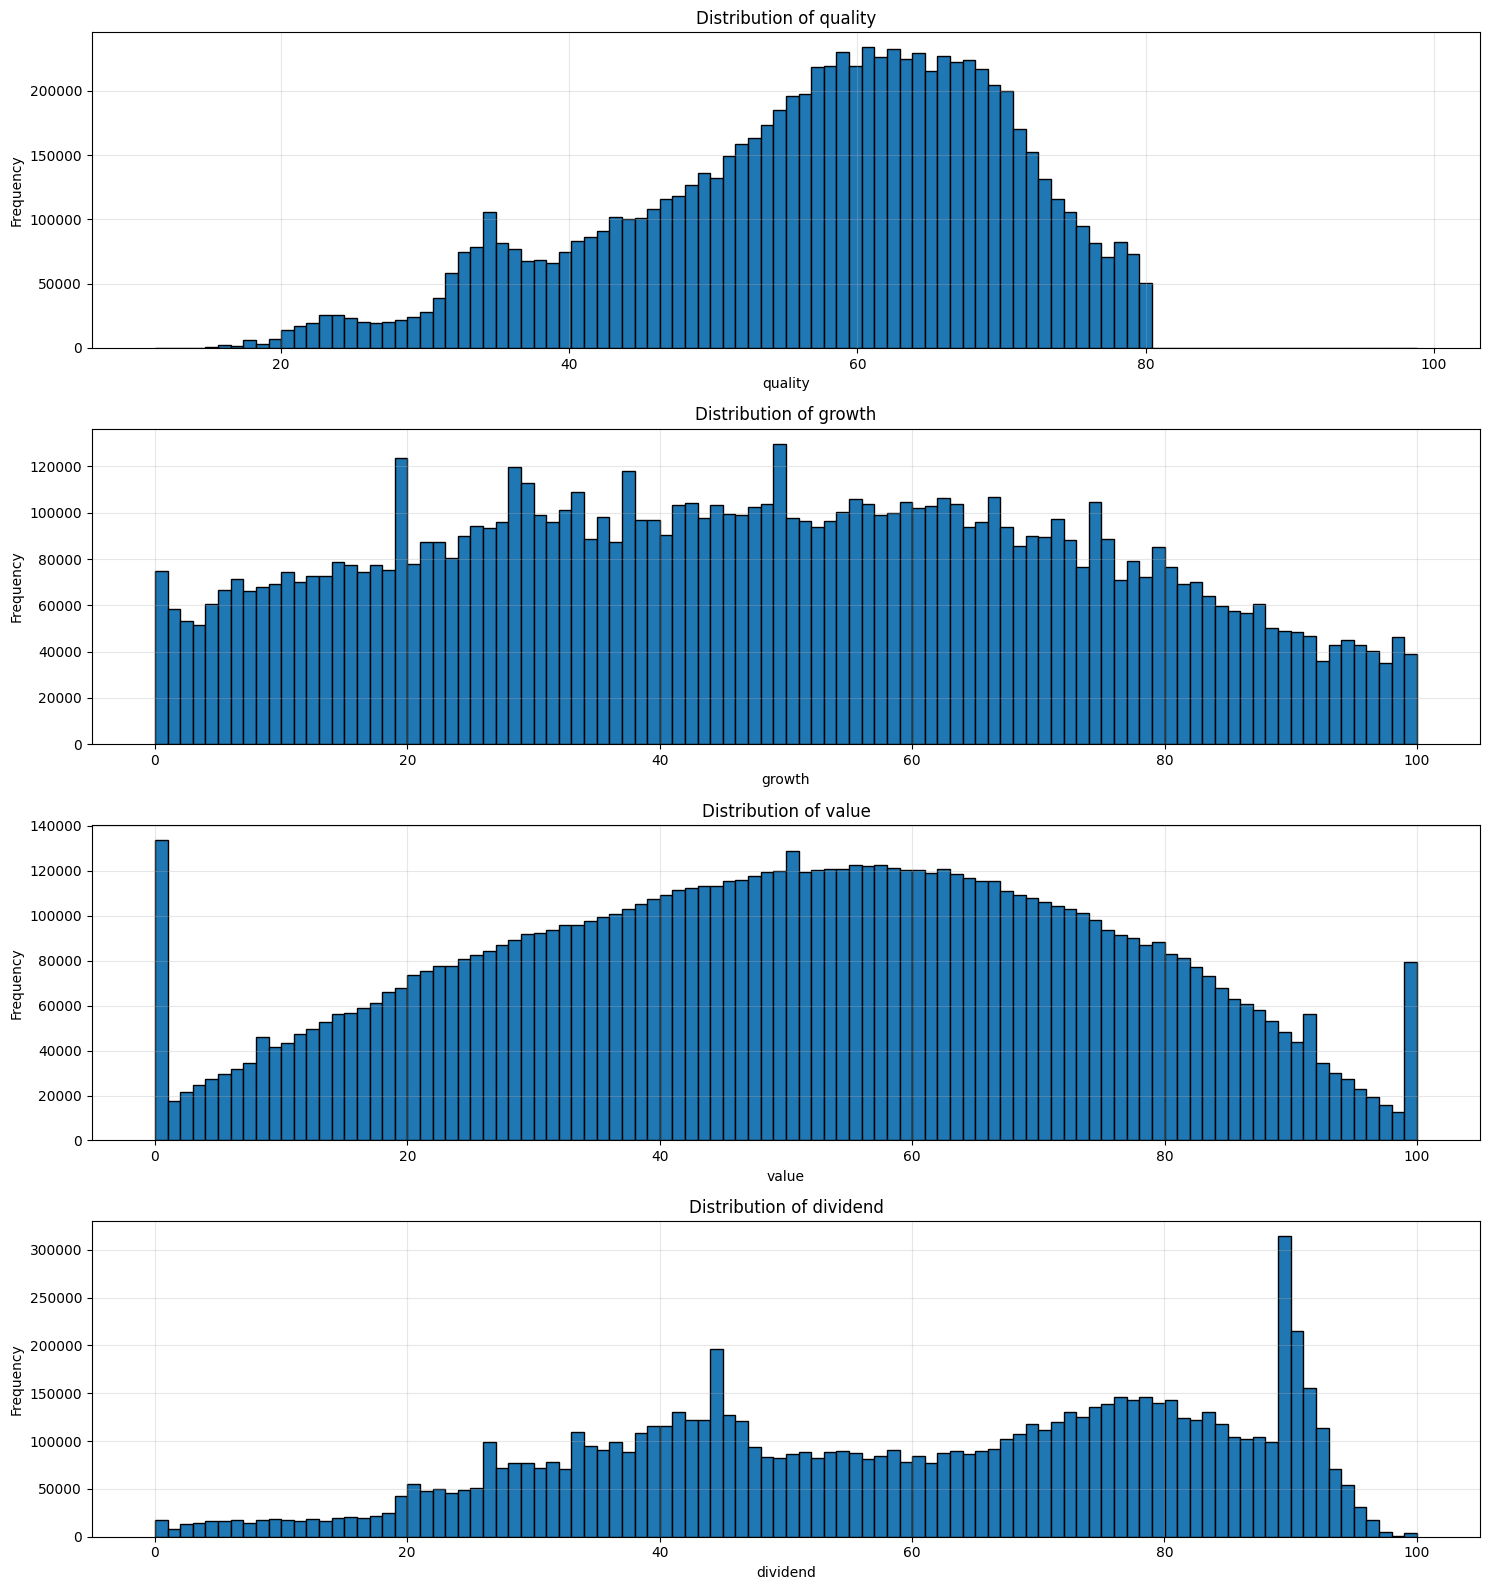
\includegraphics[width=\linewidth]{images/code/descriptive analysis/distributions/Big Data future - Scores Deep.png}
        \caption{Big Data Future - Scores Deep}
        \label{fig:scores_deep}
    \end{minipage}
\end{figure}

\noindent Around 2015-2020 interest rates were at a historical low, so there could be more companies with more debt than normal. Some central banks, particularly in Europe, experimented with negative interest rate policies on deposit facilities during this period (Figure~\ref{fig:euribor}). This possibility should be studied in more detail, but knowing that this doesn't happen for the dataset between 2020-2025 where interest rates are higher, we have a clue that this could be whats causing it (see Appendix Figure~\ref{fig:past_scores_deep}).


\begin{figure}[H]
    \centering
    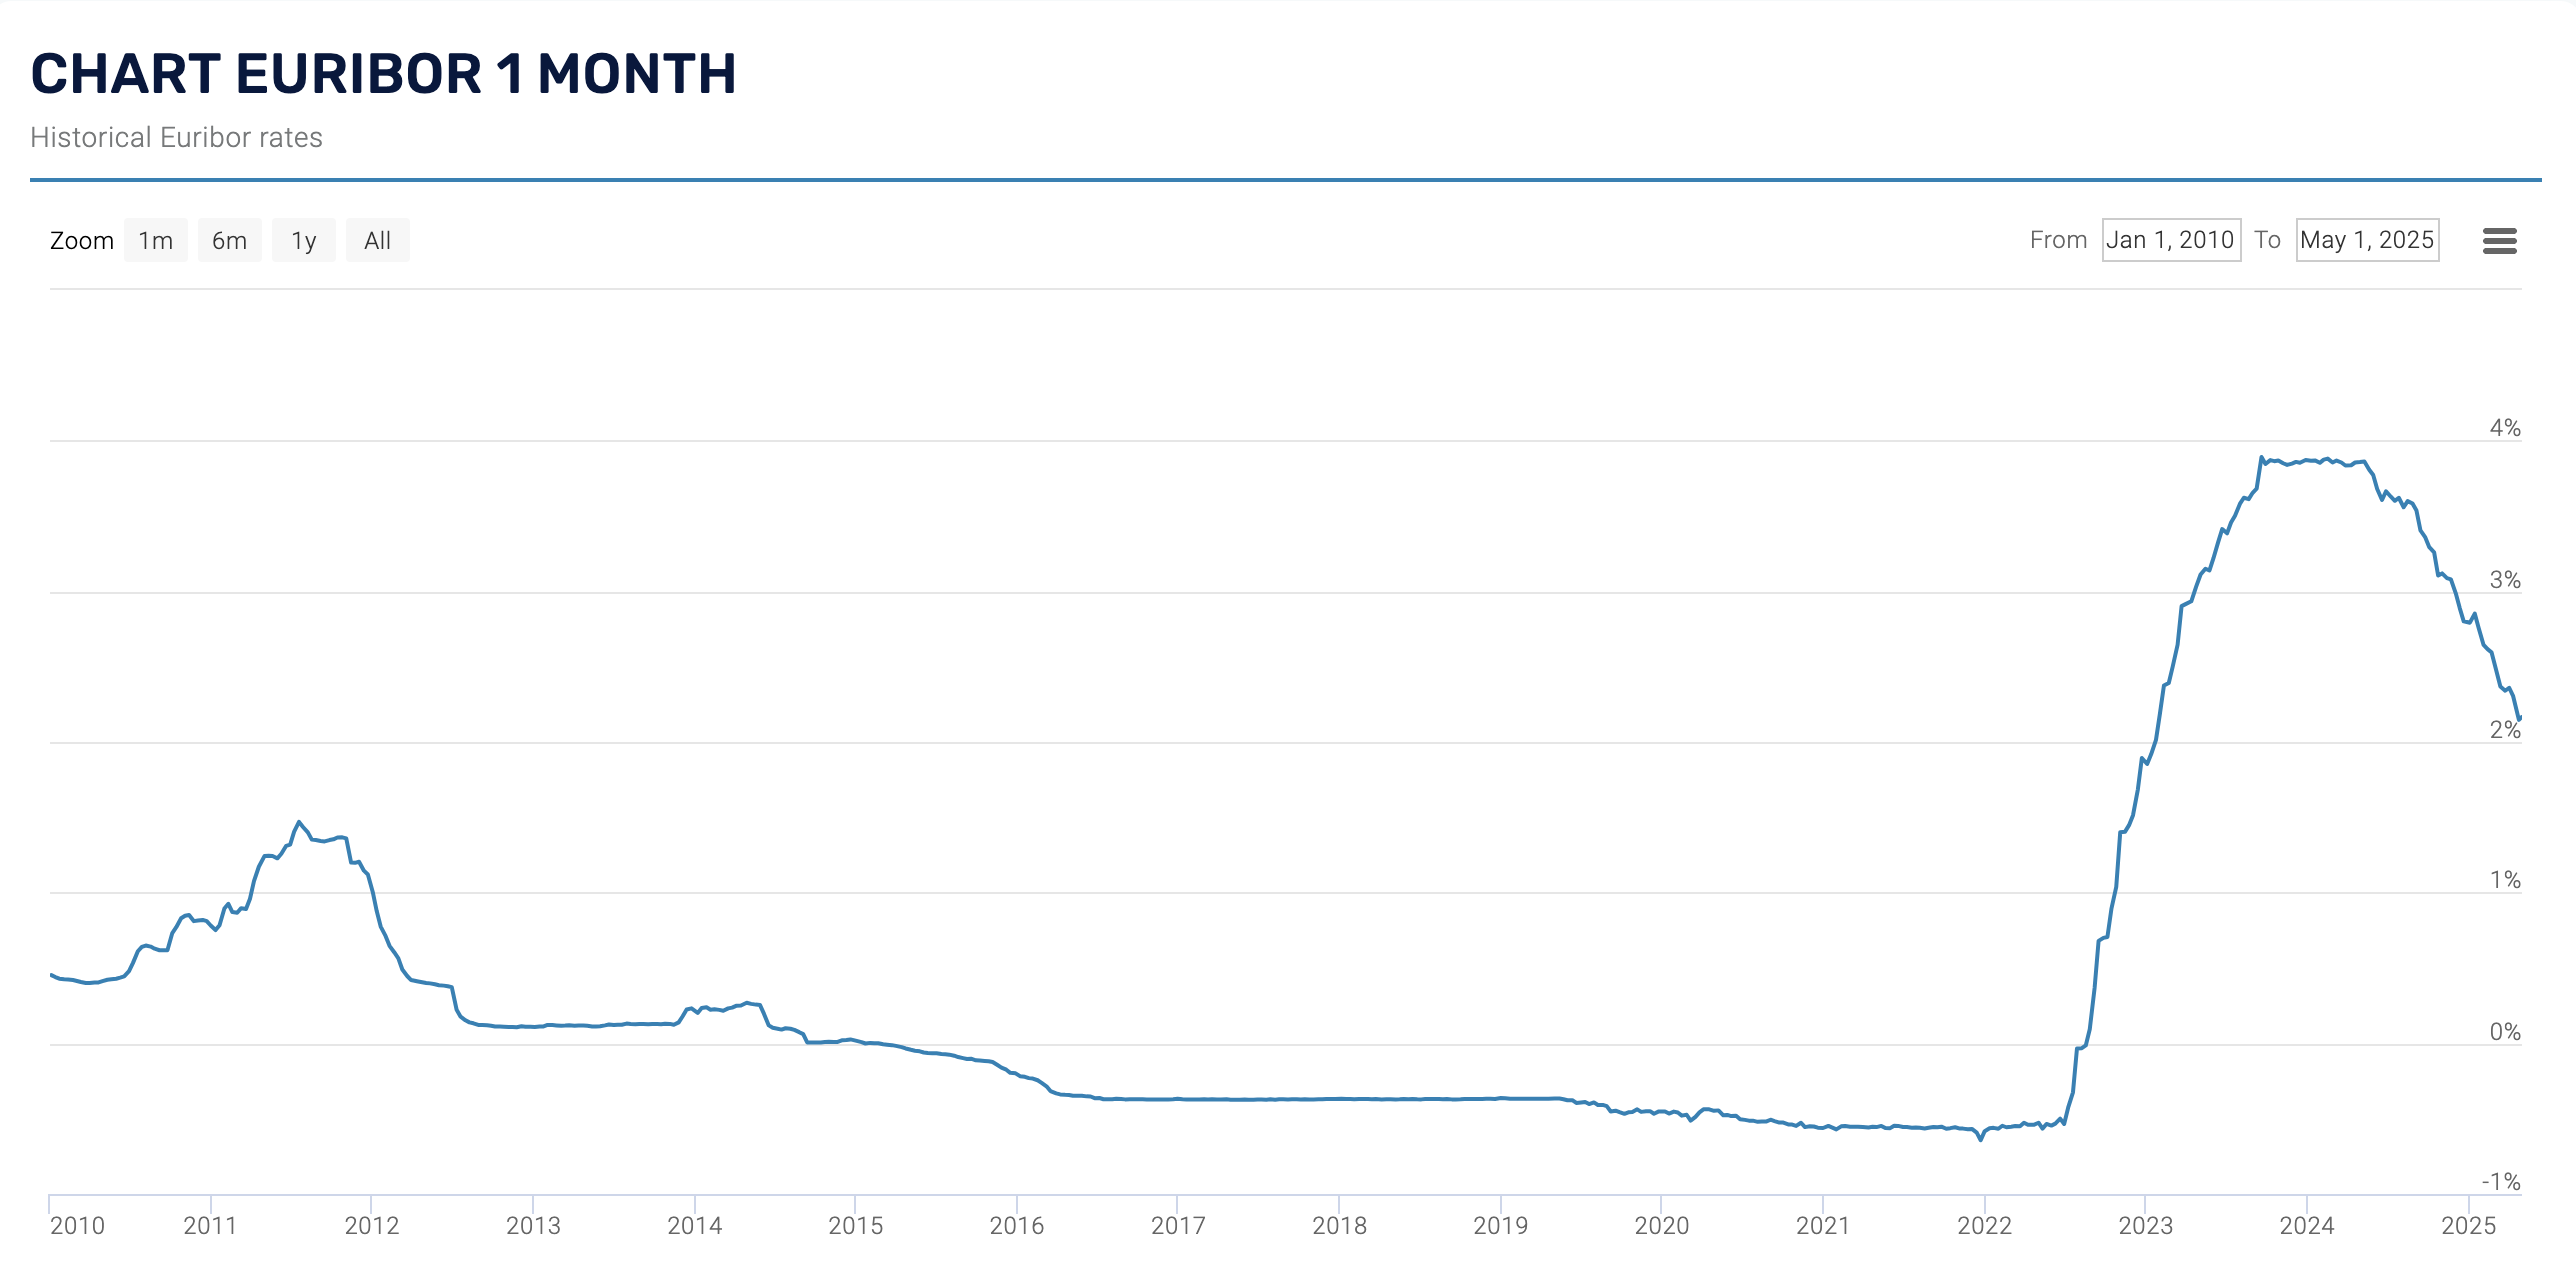
\includegraphics[width=1\linewidth]{images/macros/Euribor.png}
    \caption{EMMI - Euribor Interest Rates}
    \label{fig:euribor}
\end{figure}



\vspace{0.5cm}
\noindent Finishing with quality, there is a "deffect" in the dataset. We don't have 10 year averages for the companies that are in the 2015-2020 period --Tweenvest is only paying for data after 2012-- so the algorithm gives 0 to some of its criterias making the maximum quality be 80. But since this is happening for all of the companies, \textbf{it is not a problem for the model fitting}, altought we won't be analiyzing those criteria's performance.

\vspace{0.5cm}
\noindent Continuing with growth, we notice that there are many companies with a score of 0 and a score of 100, and something similar happens with the 0s in Diviend. For having a deeper look, we excluded those values for the Figure \ref{fig:scores_deep} where we can see that it is closer to a uniform distribution with a descend slope after 65, which means that most companies have a similar growth rate, but fewer have higher ones.

\vspace{0.5cm}
\noindent When looking at the value score, we can see that the distribution almost has an average of 50, and there is a continum of values trough the whole range, so it seems that we have a well scale for distributing the companies.

\vspace{0.5cm}
\noindent Lastly for the dividend score, as mentioned before, there are many companies that don't pay dividends. But aside from that, we have an irregular distribution for the score, with a peak arounf 85-92 meaning that there are multiple companies that respect their dividend policy.

\subsubsection{Dummies}

When it comes to the dummies we see a uniform distribution with the sectors because this condition was forced in the data creation process. But with the regions we have a different result, seeing a clear \textbf{predomination of the Asiatic region}, which happens in all of the datasets. Which could create issues for the model fitting, since it is known that in countries like China have more volatility and lower returns \textcite{chen2024economic}.

\begin{figure}[H]
    \centering
    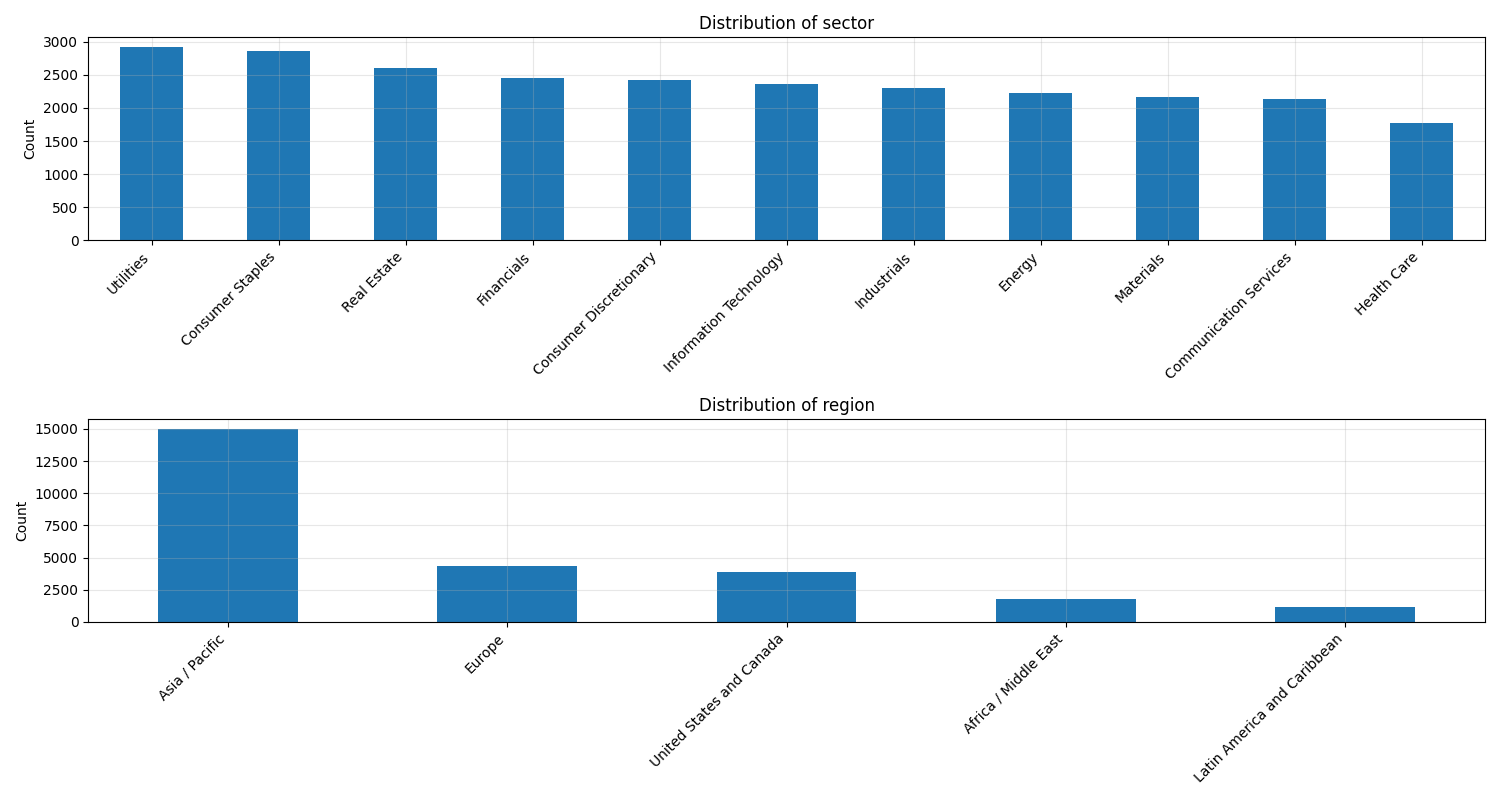
\includegraphics[width=1\linewidth]{images/code/descriptive analysis/distributions/Small Data future - Dummies.png}
    \caption{Small Data Future - Dummies}
    \label{fig:small_future_dummies}
\end{figure}

\noindent  Also, their auditors often lack true independence, especially when auditing state-owned enterprises (SOEs) or firms with strong political ties. The Chinese government tightly controls domestic accounting firms and imposes restrictions on foreign auditors. Even international firms like \textit{PwC-China} operate under local joint ventures, often with limited autonomy, as reviewd in \textcite{LIU2012782}. So we will have to check if the dummies variables are enough to take this effect into account, or if we need a different approach for modeling the geographical effects.

\vspace{0.5cm}
\noindent It is worth noting that the distribution of companies across sectors varies significantly over time, as shown in Appendix Figures \ref{fig:future_dummies} and \ref{fig:past_dummies}. This temporal variation in sector representation presents an interesting opportunity for future research.

\subsubsection{Profits}

\noindent When analyzing the profit distributions across different time horizons, we observe that the distributions contain a numerous amount of outliers that don't let us see the distributions clearly (Appendix Figures \ref{fig:big_data_future_profits_boxplot} and \ref{fig:big_data_future_profits}). So just for this descriptive analysis purposes, \textbf{we used the IQR method} mentioned in previous chapters to remove the outliers.

\begin{figure}[H]
    \centering
    \begin{minipage}{0.48\textwidth}
        \centering
        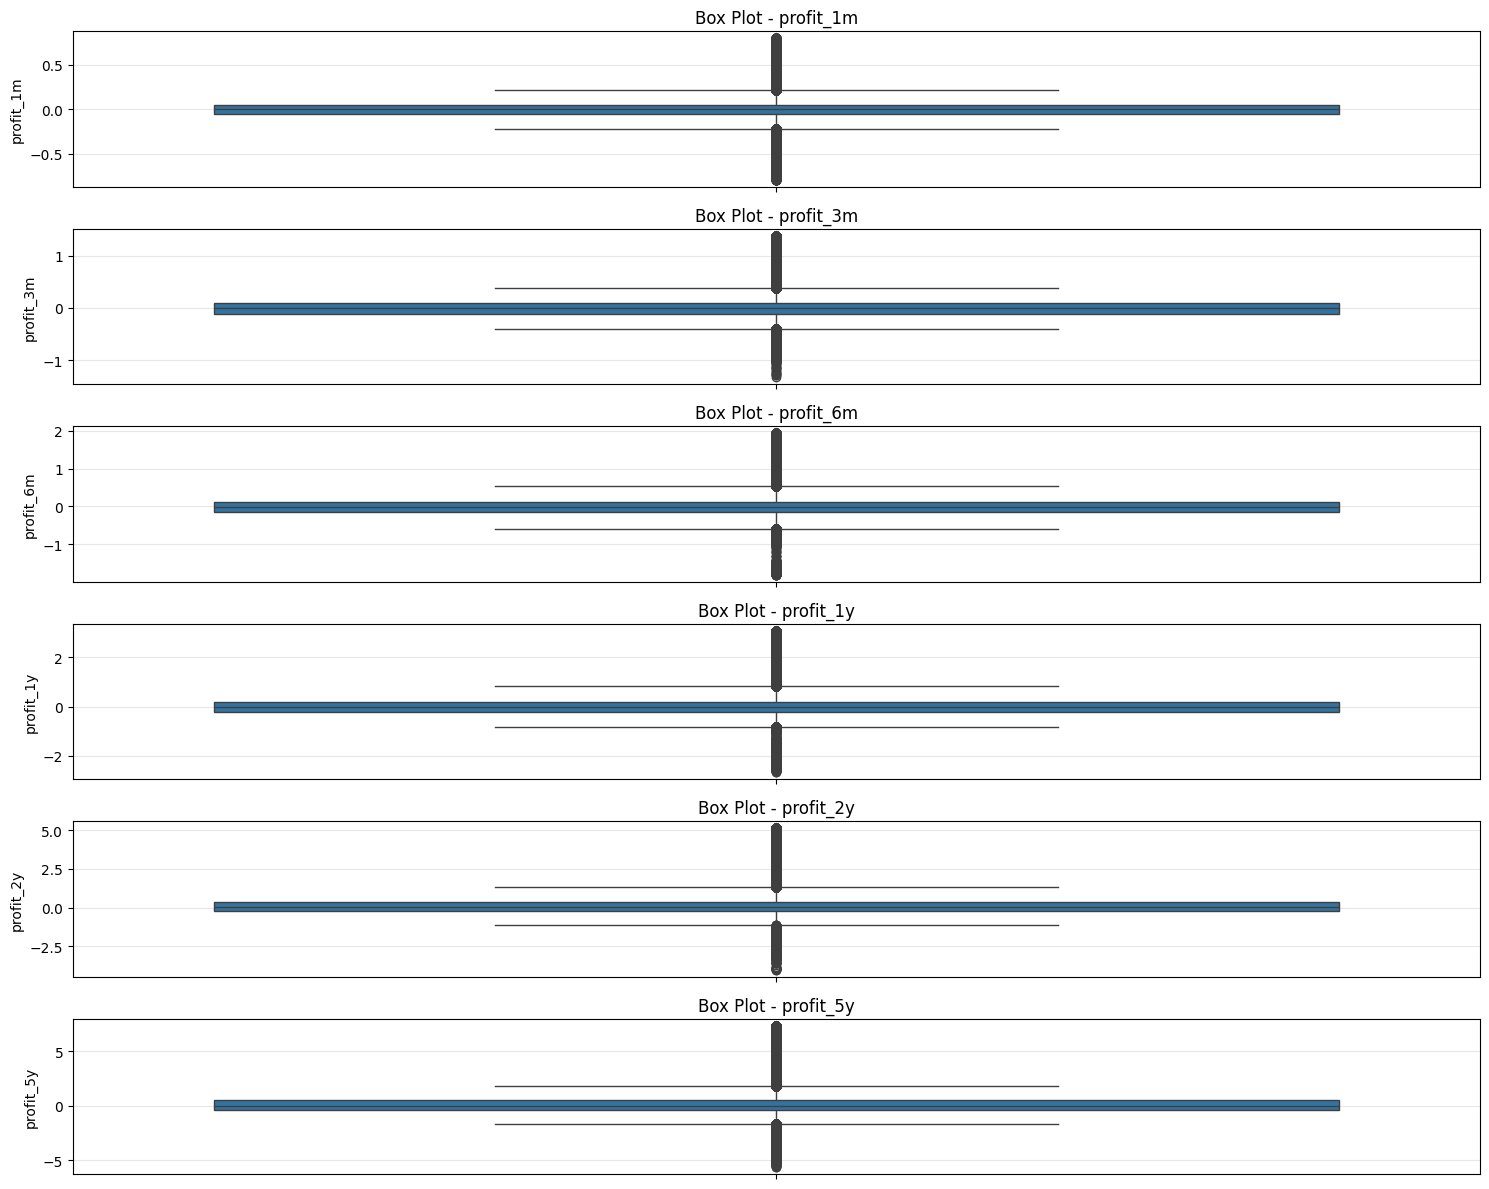
\includegraphics[width=0.8\linewidth]{images/code/descriptive analysis/distributions/Big Data future IQR - Profits Boxplot.png}
        \caption{Big Data Future IQR - Profits Boxplot}
        \label{fig:big_data_future_iqr_profits_boxplot}
    \end{minipage}\hfill
    \begin{minipage}{0.48\textwidth}
        \centering
        \includegraphics[width=0.8\linewidth]{images/code/descriptive analysis/distributions/Big Data Future IQR - Profits.png}
        \caption{Big Data Future IQR - Profits}
        \label{fig:big_data_future_iqr_profits_iqr}
    \end{minipage}
\end{figure}


\vspace{0.5cm}
\noindent Interestingly, we notice that the short-term profit distributions (1-month and 3-month) are more symmetric and closer to normal distributions, which is consistent with the efficient market hypothesis suggesting that short-term price movements are largely random. 

\vspace{0.5cm}
\noindent However, as we extend to longer time horizons, the distributions become more positively skewed, which aligns with the general expectation that most companies don't have good returns, except of the market winners that tend to generate extraordinary positive returns due to the mentioned \textbf{economic moats}. This is particularly evident in the longer-term profit distributions (2-year and 5-year), where we see a longer tail extending toward higher positive returns.


\vspace{0.5cm}
\noindent There is also a tendency to having less negative returns compared to the positive ones the longer the time-frame. Logically, companies with bad returns don't last long.

\subsection{Correlations}

For analizing the correlations between the variables, we will start firstly with just the cleaned big datasets, and then we will use also the datasets without the outliers, since these are the ones that will be used for the model fitting.

\vspace{0.5cm}
\noindent Here is the only section that we will be using the past Datasets, to see if past profits are being reflected in current scores.
\subsubsection{Clean Datasets}

\begin{figure}[H]
    \centering
    \begin{minipage}{0.48\textwidth}
        \centering
        \includegraphics[width=\linewidth]{images/code/descriptive analysis/correlations/Big Data Past.png}
        \caption{Big Data Past - Correlations}
        \label{fig:big_data_past_correlations}
    \end{minipage}\hfill
    \begin{minipage}{0.48\textwidth}
        \centering
        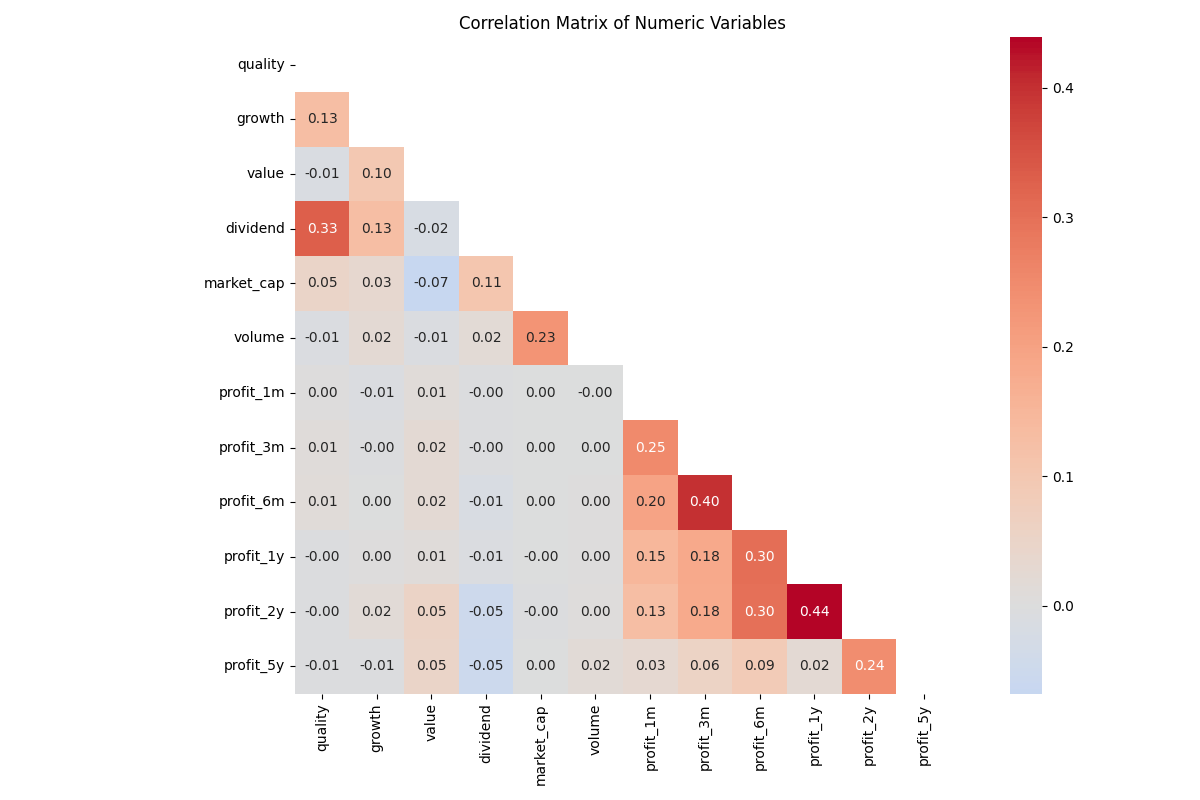
\includegraphics[width=\linewidth]{images/code/descriptive analysis/correlations/Big Data future.png}
        \caption{Big Data Future - Correlations}
        \label{fig:big_data_future_correlations}
    \end{minipage}
\end{figure}

\noindent We can appretiate three main expected correlations:
\begin{itemize}
    \item \textbf{Companies with good quality} --that is so, they have consisten growth, good liquidity and healthy debt-- \textbf{are more likely to give dividends}.
    \item There is a strong relationship betwen the market cap of a company and the volume of the shares traded.
    \item \textbf{Companies have inertia}, or how it is called \textit{Momentum}, meaning that the profit of a company is positively correlated with the profit of the previous period.
\end{itemize}

\subsubsection{Outliers Datasets}
But as it has been seen multiple times through the analysis, the outliers create a big bias that doesn't allow us to see the real correlations occurring for "normal companies". So as shown in the table \ref{tab:datasets_summary}, we will use the Big datasets fitered with the Isolation Forest method to remove outliers as a first approach, but for the model fitting we will use the multi-criteria outlier detection.

\begin{figure}[H]
    \centering
    \begin{minipage}{0.48\textwidth}
        \centering
        \includegraphics[width=\linewidth]{images/code/descriptive analysis/correlations/Big Data Past - IF.png}
        \caption{Big Data Past IF - Correlations}
        \label{fig:big_data_past_if_correlations}
    \end{minipage}\hfill
    \begin{minipage}{0.48\textwidth}
        \centering
        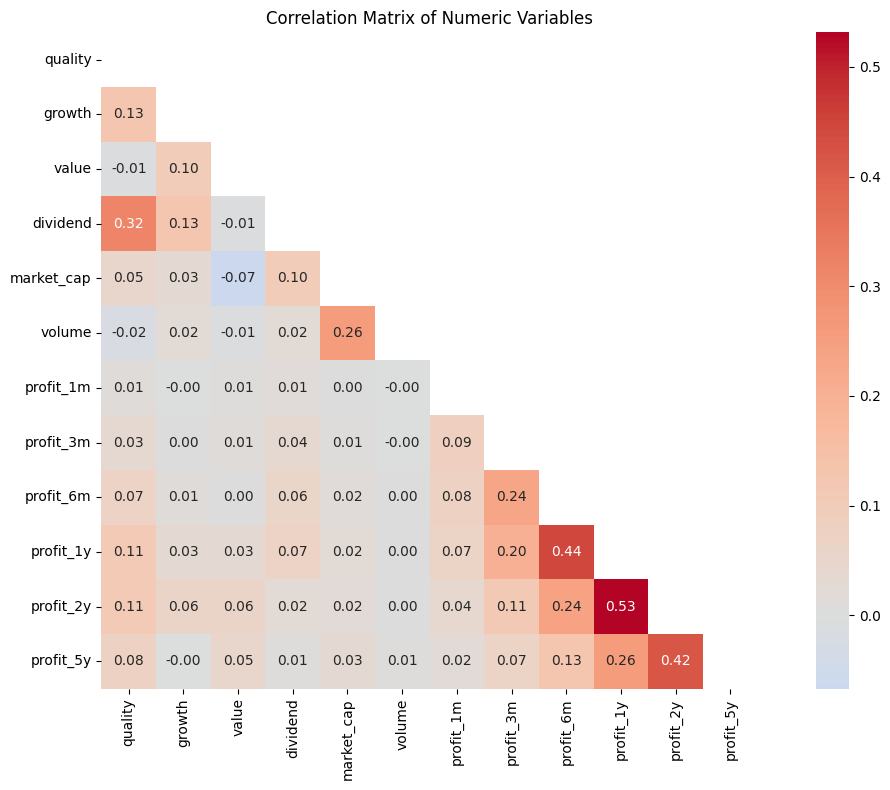
\includegraphics[width=\linewidth]{images/code/descriptive analysis/correlations/Big Data future - IF.png}
        \caption{Big Data Future IF - Correlations}
        \label{fig:big_data_future_if_correlations}
    \end{minipage}
\end{figure}

\noindent As expected, the correlations already seen stay similar with a slight increase in the \textit{Momentum}, showing more importance of it than other variables. But actually, there are \textbf{new correlations seen} for both datasets:

\begin{itemize}
    \item  \textbf{Accumulated profits affect the scores}. In the past dataset we can see that long term past profits translate into higher quality and dividend scores-- as expected by their correlation. But also, they make the value score to decrease. This could be explained by two effects:
    \begin{itemize}
        \item \textbf{Bull markets}. As explained in the second chapter, a company can experience good returns in the stock market that are not followed by good financial growth. This makes their value multiples to raise, making their value score to decrease.
        \item \textbf{The company is not able to maintain its profitability}. If a company has had good past profits, but is not able to maintain them, the market will eventually realize that and the company will have a lower value score.
    \end{itemize}
    \item \textbf{Long term stock returns affect the company's growth}. This is a very interesting result, since it explains the reason why companies try to go to the market to raise capital and help the company grow.
    \item \textbf{Quality is correlated to future profits}. This could be explained by the fact that a company with good quality is more likely to have good future profits, but also by the fact that the market is efficient and the price of a company will reflect all of the information available.
    \item There is a \textbf{mild correlation between most scores}, which could be explain by the fact that a company that does well in one aspect, is more likely to do well in the others. This correlation won't affect the models because they are separated by score.
\end{itemize}

\noindent Althought we have to make clear that these correlations do not stand along all of the datasets separated by region (see Appendix Figures from \ref{fig:small_data_future_usa_correlations} to \ref{fig:small_data_future_as_multi_correlations}), so we aren't sure yet if these relationships will be properly explained with linear models.

\subsection{Data clusters}
Finally, we are going to try to compare these results with the pairplots of the datasets, to look for clusters of data when comparing many variables at once.

\begin{figure}[H]
    \centering
    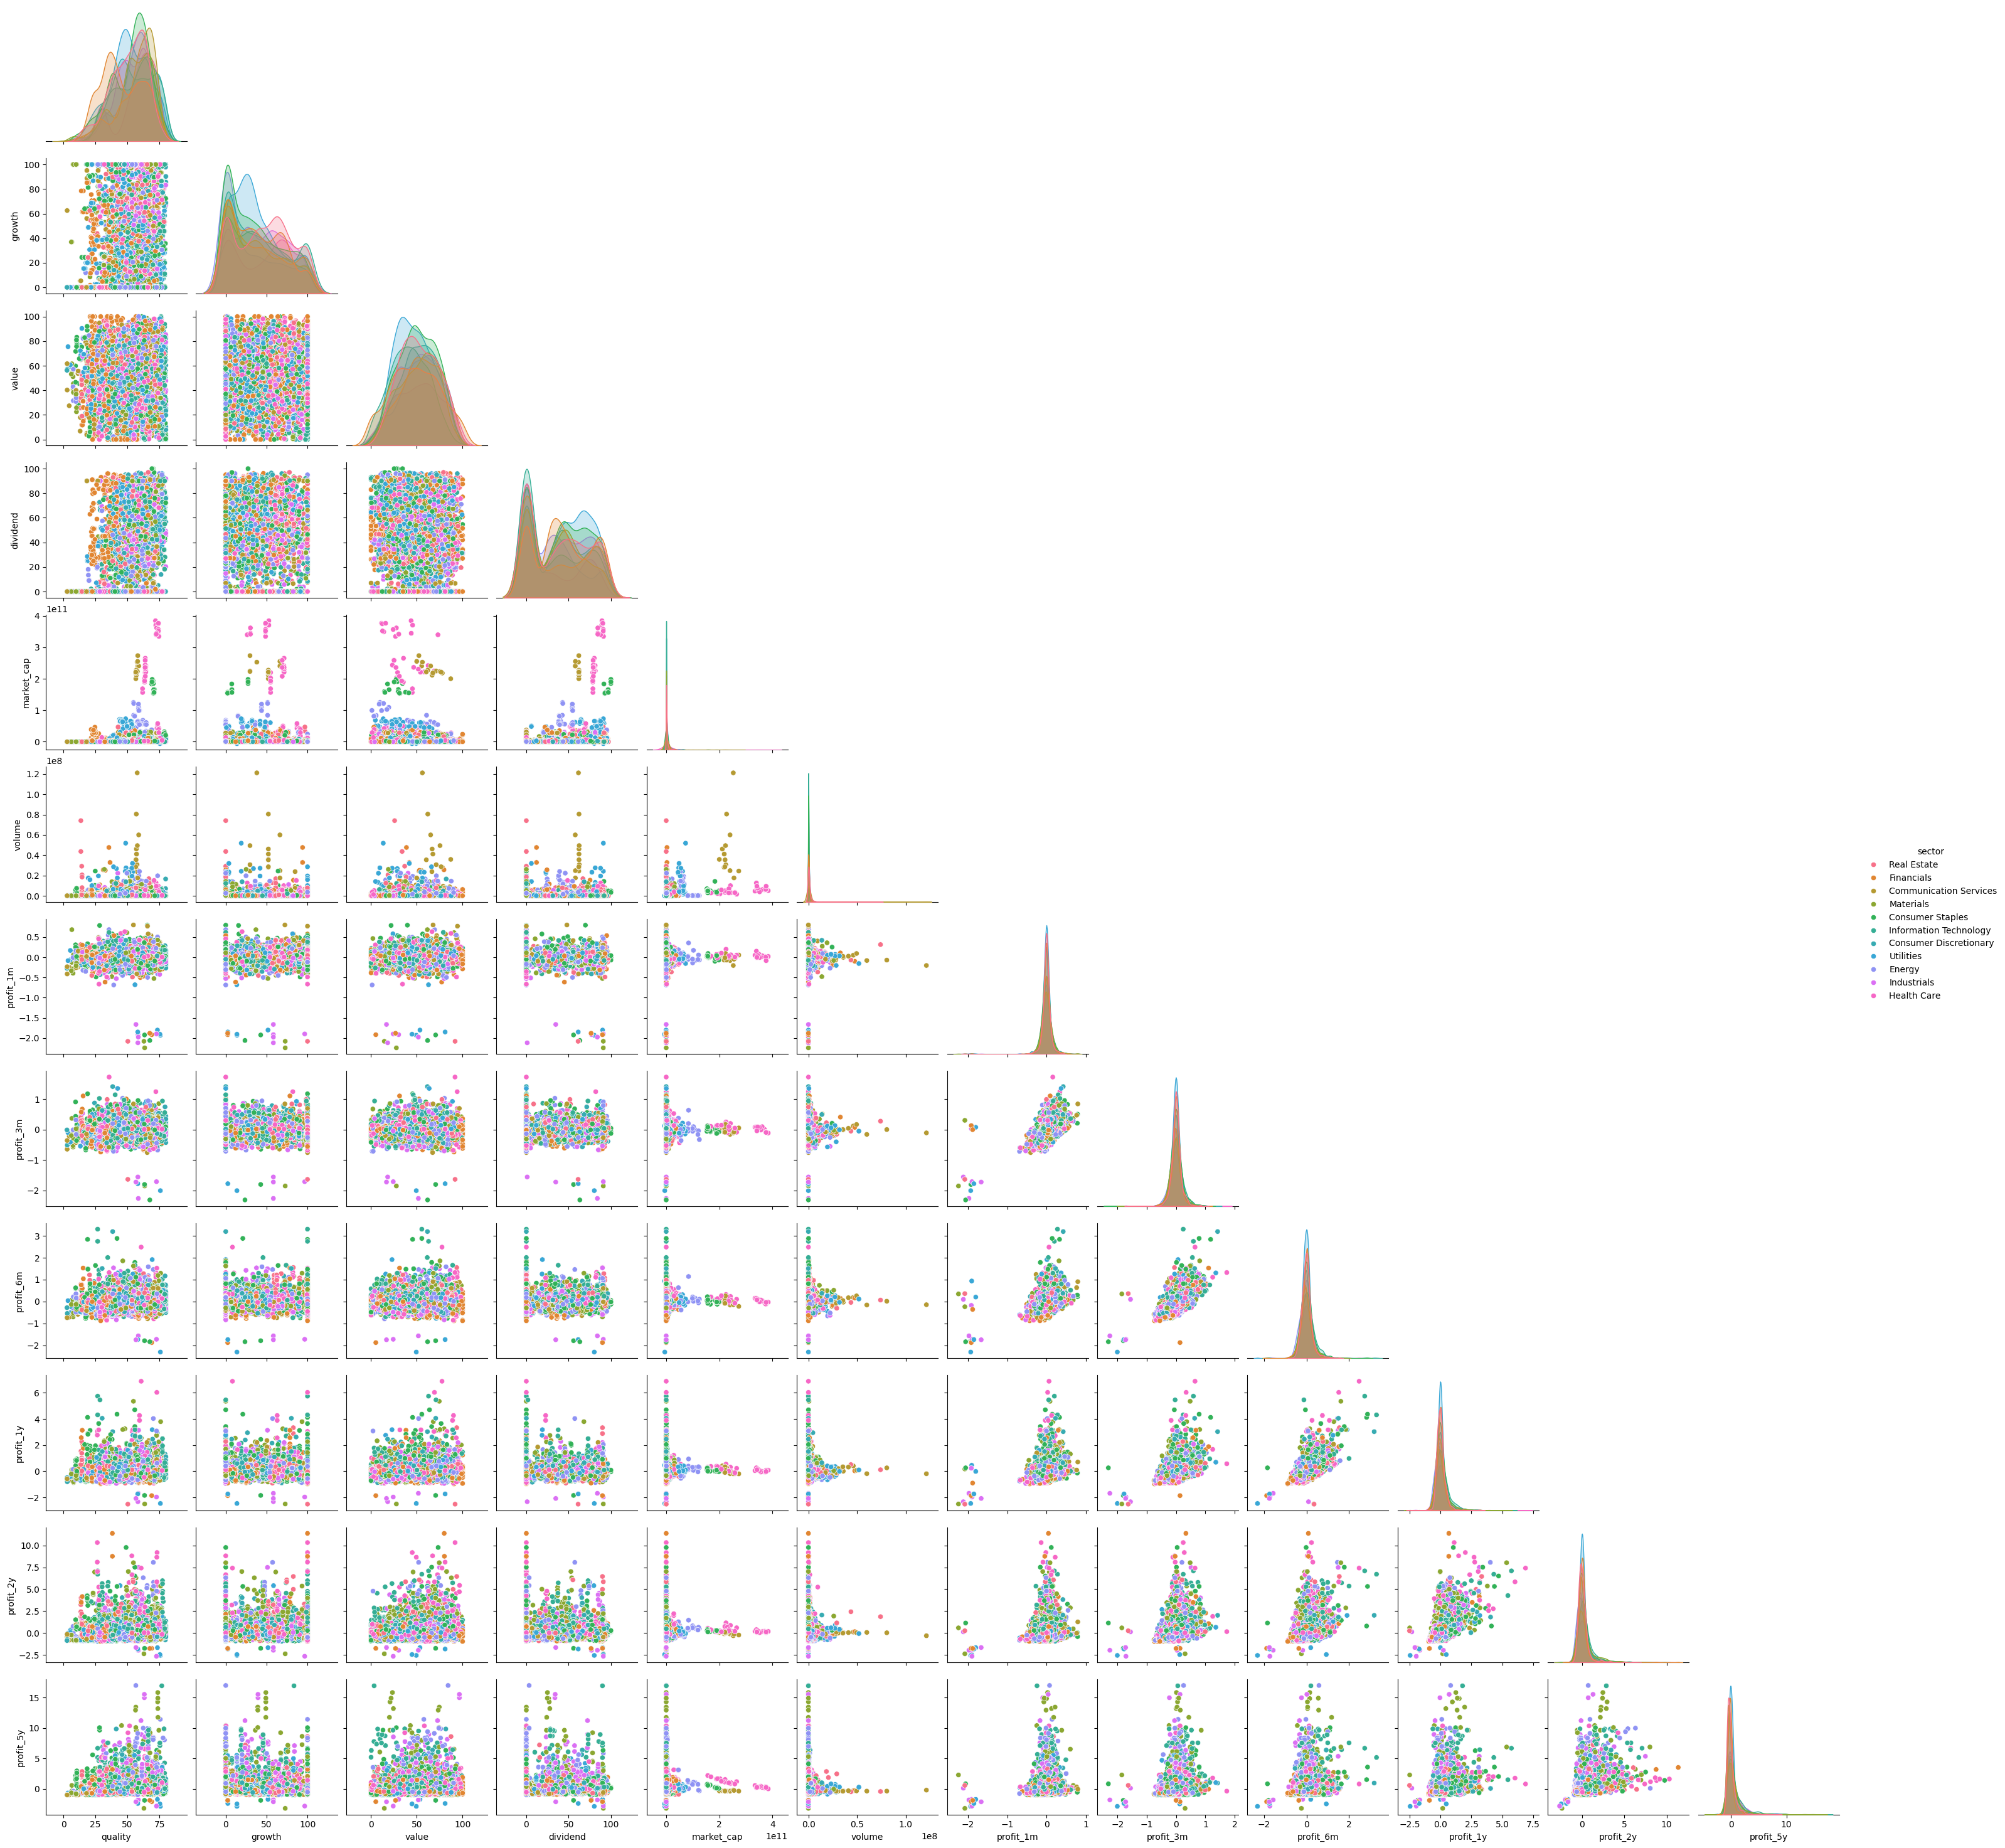
\includegraphics[width=1\textwidth]{images/code/descriptive analysis/correlations/Small Data future - Multi - pairplot.png}
    \caption{Pairplot of Small Data Future - Multi}
    \label{fig:pairplot_small_data_future_multi}
\end{figure}

\noindent Here it is harder to eye-see the data structure that could form clusters since there are many datapoints, but there are some exceptions:
\begin{itemize}
    \item \textbf{Profits}. We can see linear correlations between some of the different profits, but for longer horizons the relationships are no longer liner. Which is expected since the further the horizon, more variables take part in the calculation of the profit.
    \item \textbf{Market Cap}. Companies with bigger market caps tend to have higher quality and dividend scores. Bigger companies should have a more stable financial situaition, otherwise they wouldn't be as big in the long term. Also there are some sectors that tend to have higher market caps than others, like in Health Care or Consumer Staples.
    \item \textbf{Sector}. It seems that there could be a pattern seen in the sectors distribution for each scores, but it is not clear.
\end{itemize}

\noindent Althought, these results are not as clear and they also variate deppending on the dataset. Showing early results of non-linear relationships with the dummy variables.

\section{Predictive Models}

\subsection{Linear Regression}

\subsection{The problem with ARIMA}

\subsection{GAM}

\subsection{Neural Network}

\section{Back-testing}



% ############################### DISCUSSION #######################
\chapter{Discussion}
% Analysis and interpretation

% ############################### CONCLUSION #######################
\chapter{Conclusion}
% Summary and conclusions

% ############################### BIBLIOGRAPHY #######################
\printbibliography[heading=bibintoc, title=Bibliography]
\label{sec:biblio}
\newpage

% ############################### APPENDICES #######################
\part{Appendix}
% % \def\thechapter{\Alph{chapter}}
% \makeatletter
% \renewcommand{\@chapapp}{Appendix}
% \makeatother

\chapter{Code Listings}
% -------------------------- Scores Calculation Job --------------------------
\section{Historical Scores Job Implementation}
\label{app:historical_scores_job}

\noindent The following code snippets shows the complete implementation of the historical scores job that was used to populate the database with historical factor scores data:

\subsection{Enqueueing Historical Scores Job}

\begin{lstlisting}[language=Python, caption=Enqueueing Historical Scores Job, label={lst:enqueue_calculate_index_scores_task}]
@job("historical_scores", timeout="3h")
def enqueue_calculate_index_scores_task(
    start_date: datetime.date,
    end_date: datetime.date,
    index_names: list[str] | None = None,
    region_names: list[str] | None = None,
    total_stocks: int | None = None,
    seed: float | None = None,
    daily: bool = False,
):
    logger.info(
        "[H1] Starting enqueue_year_tasks from %s to %s",
        start_date,
        end_date,
    )

    days = get_range_from_dates(
        start_date,
        end_date,
        delta=relativedelta(days=1) if daily else relativedelta(months=1),
    )
    days.reverse()

    if not index_names:
        index_names = list(
            Index.objects.exclude(name__in=[Index.INDEX_ALL, "Other"])
            .only("name")
            .values_list("name", flat=True)
        )
    logger.info("[H1] Enqueuing tasks for %s indexes", len(index_names))

    stocks_per_index = (
        int(total_stocks / len(index_names)) if total_stocks else None
    )

    stock_count = 0
    total_stocks_dict = {}
    for index_name in index_names:
        stock_ids = get_stock_ids_for_index(
            index_name,
            stocks_per_index,
            start_date,
            end_date,
            seed,
            region_names,
        )
        if not stock_ids:
            raise ValueError(
                f"[H1] No stocks found for index '{index_name}' after {start_date}"
            )
        total_stocks_dict[index_name] = stock_ids
        for day in days:
            calculate_index_scores_task.delay(
                index_name=index_name,
                day=day,
                stock_ids=stock_ids,
            )

        stock_count += len(stock_ids)

    logger.info(
        "[H1] Enqueued days %s for stocks:%s .", len(days), stock_count
    )

    return {
        "stocks_processed": stock_count,
        "days": len(days),
        "total_stocks": total_stocks_dict,
    }
\end{lstlisting}

\noindent This job function is responsible for:
\begin{itemize}
    \item Accepting date ranges and configuration parameters for historical score calculation
    \item Generating a list of dates to process (either daily or monthly intervals)
    \item Retrieving stock IDs for each index based on the specified criteria
    \item Enqueuing individual calculation tasks for each day and index combination
    \item Providing detailed logging and return statistics about the processing
\end{itemize}

\subsection{Calculate Index Scores Data}
\begin{lstlisting}[language=Python, caption=Calculate Index Scores Data, label={lst:calculate_index_scores_task}]

@job("historical_scores", timeout="45m")
def calculate_index_scores_task(
    index_name: str,
    day: datetime.date,
    stock_ids: list[int],
):
    start_time = time.perf_counter()
    logger.info(
        "[H2] Calculating index",
        extra={
            "index": index_name,
            "day": day,
            "stocks": len(stock_ids),
        },
    )

    # ---------------- Index calculation ----------------- #
    index_stats = get_indexes_information(
        index_names=[index_name], calculation_date=day
    )
    index_quality = get_quality_ratios_by_index(
        index_names=[index_name], calculation_date=day
    )
    stats = index_stats.get(index_name)
    quality = index_quality.get(index_name)

    # ----------------------------------------------------- #
    if (
        not stats
        or not quality
        or all(value is None for value in quality.values())
        or all(
            value is np.nan
            for stat in stats.values()
            for value in stat.values()
        )
    ):
        raise RuntimeError(
            f"[H2] Missing index data for {index_name} on {day},  stats: {stats}, quality: {quality}"
        )

    calculate_stocks_scores_task.delay(
        day=day,
        stats=stats,
        quality=quality,
        stock_ids=stock_ids,
    )
    return {
        "index_calculated": index_name,
        "total_time": time.perf_counter() - start_time,
    }
\end{lstlisting}

\noindent This job function is responsible for:
\begin{itemize}
    \item Calculating all the necessary index stats data
    \item Enqueuing the calculation of the stocks scores for the given index and date
    \item Providing detailed logging and return statistics about the processing
\end{itemize}

\subsection{Calculate Stocks Scores Task}
\begin{lstlisting}[language=Python, caption=Calculate Stocks Scores Task, label={lst:calculate_stocks_scores_task}]
@tracer.start_as_current_span("calculate_stocks_scores_task")
@job("historical_scores", timeout="4h")
def calculate_stocks_scores_task(
    day: datetime.date,
    stats: dict,
    quality: dict,
    stock_ids: list[int],
):
    """
    Job 3: For each stock, calculate scores and bulk save.
    """
    start_time = time.perf_counter()
    logger.info(
        "[H3] Calculating scores",
        extra={"day": day, "stocks": len(stock_ids)},
    )

    if not stock_ids:
        return {
            "stocks_processed": 0,
        }
    # Select related for trying to avoid multiple queries to the DB
    stocks = Stock.objects.filter(id__in=stock_ids).select_related(
        "share_type",
        "share_type__company",
        "share_type__company__industry",
        "share_type__company__industry__industry_group",
        "share_type__company__industry__industry_group__sector",
    )
    factor_scores = []
    for stock in stocks:
        score = calculate_scores(
            stock,
            stats,
            quality,
            calculation_date=day,
            bulk_create_or_update=True,
        )
        if not score:
            logger.warning(
                "[H3] No score for calculated",
                extra={"stock_id": stock.pk, "day": day, "score": score},
            )
            continue  # Not as important as the others, need to check errors in DataDog
        factor_scores.append(score)

    bulk_create_or_update(
        model=FactorScore,
        object_list=factor_scores,
        unique_fields=["stock", "date"],
        update_fields=["quality", "growth", "value", "dividend"],
    )

    return {
        "stocks_processed": len(stock_ids),
        "total_time": time.perf_counter() - start_time,
        "time_per_stock": (time.perf_counter() - start_time) / len(stock_ids),
    }
    
\end{lstlisting}

\noindent This job function is responsible for:
\begin{itemize}
    \item Calculating the factor scores for each stock in the given index and date
    \item Bulk saving the factor scores for the given index and date
    \item Providing detailed logging and return statistics about the processing
\end{itemize}

\section{Workers Management}

In this section we have 2 different configurations for the workers management, since we had to switch servers.

\subsection{Tweenvest's Production Server}
\begin{lstlisting}[language={}, caption=Production Workers Management, label={lst:tweenvest_production_workers_management}]
[program:worker1]
command=python manage.py rqworker internal_tasks ciq_priority fmp_priority ciq indices_partial indices_full historical_scores fmp emails --with-scheduler
directory=/app
autostart=true
autorestart=true
redirect_stderr=true
stdout_logfile=/dev/fd/1
stdout_logfile_maxbytes=0
environment = SERVICE_NAME="tweenvest-worker"

[program:worker2]
command=python manage.py rqworker internal_tasks ciq_priority fmp_priority ciq indices_partial indices_full historical_scores fmp emails --with-scheduler
autostart=true
directory=/app
autorestart=true
redirect_stderr=true
stdout_logfile=/dev/fd/1
stdout_logfile_maxbytes=0
environment = SERVICE_NAME="tweenvest-worker"

[program:worker3]
command=python manage.py rqworker internal_tasks ciq_priority fmp_priority ciq indices_partial fmp emails historical_scores --with-scheduler
autostart=true
directory=/app
autorestart=true
redirect_stderr=true
stdout_logfile=/dev/fd/1
stdout_logfile_maxbytes=0
environment = SERVICE_NAME="tweenvest-worker"

[program:worker4]
command=python manage.py rqworker ciq_priority fmp_priority ciq indices_partial fmp emails historical_scores --with-scheduler
autostart=true
directory=/app
autorestart=true
redirect_stderr=true
stdout_logfile=/dev/fd/1
stdout_logfile_maxbytes=0
environment = SERVICE_NAME="tweenvest-worker"

[program:worker5]
command=python manage.py rqworker fmp_priority ciq_priority ciq fmp emails --with-scheduler
autostart=true
directory=/app
autorestart=true
redirect_stderr=true
stdout_logfile=/dev/fd/1
stdout_logfile_maxbytes=0
environment = SERVICE_NAME="tweenvest-worker"

[program:worker6]
command=python manage.py rqworker emails --with-scheduler
autostart=true
directory=/app
autorestart=true
redirect_stderr=true
stdout_logfile=/dev/fd/1
stdout_logfile_maxbytes=0
environment = SERVICE_NAME="tweenvest-worker"

[program:worker7]
command=python manage.py rqworker ciq_priority ciq emails summaries --with-scheduler
directory=/app
autostart=true
autorestart=true
redirect_stderr=true
stdout_logfile=/dev/fd/1
stdout_logfile_maxbytes=0
environment = SERVICE_NAME="tweenvest-worker"

[program:worker8]
command=python manage.py rqworker ciq_priority ciq emails summaries --with-scheduler
directory=/app
autostart=true
autorestart=true
redirect_stderr=true
stdout_logfile=/dev/fd/1
stdout_logfile_maxbytes=0
environment = SERVICE_NAME="tweenvest-worker"

[program:worker9]
command=python manage.py rqworker historical_scores ciq_priority summaries ciq emails --with-scheduler
directory=/app
autostart=true
autorestart=true
redirect_stderr=true
stdout_logfile=/dev/fd/1
stdout_logfile_maxbytes=0
environment = SERVICE_NAME="tweenvest-worker"

[program:worker10]
command=python manage.py rqworker summaries ciq_priority fmp_priority ciq fmp emails --with-scheduler
directory=/app
autostart=true
autorestart=true
redirect_stderr=true
stdout_logfile=/dev/fd/1
stdout_logfile_maxbytes=0
environment = SERVICE_NAME="tweenvest-worker"
\end{lstlisting}

\subsection{Personal Development Server}
\begin{lstlisting}[language={}, caption=Hetzner Workers Management, label={lst:hetzner_workers_management}]
[program:worker1]
command=python manage.py rqworker historical_scores
process_name=%(program_name)s_%(process_num)02d
numprocs=16
directory=/app
autostart=true
autorestart=true
redirect_stderr=true
stdout_logfile=/dev/fd/1
stdout_logfile_maxbytes=0
environment = SERVICE_NAME="tweenvest-worker"
\end{lstlisting}


% -------------------------- Data Export Job --------------------------
\section{Data Export Job Implementation}
\label{app:data_export_job}

\noindent The following code shows the complete implementation of the data export job that was used to create the final dataset, including the price estimation for missing values due to weekends and holidays:

\begin{lstlisting}[language=Python, caption=Data Export Job Implementation]
def export_factors_and_pricehistory_task(
    stocks_id: list[int],
    start_date: datetime.date,
    end_date: datetime.date,
    export_name: str,
    daily: bool = False,
):
    """
    Export FactorScore, PriceHistory y rentabilidades a CSV sin cargar todo en memoria.
    """
    start_time = time.perf_counter()
    print("Starting CSV export...")

    periods = {
        "profit_1m": relativedelta(months=1),
        "profit_3m": relativedelta(months=3),
        "profit_6m": relativedelta(months=6),
        "profit_1y": relativedelta(years=1),
        "profit_2y": relativedelta(years=2),
        "profit_5y": relativedelta(years=5),
    }

    factor_fields = [
        "stock__ticker",
        "stock__share_type__company__name",
        "stock__share_type__company__industry__industry_group__sector__name",
        "stock__share_type__company__country__region",
        "date",
        "quality",
        "growth",
        "value",
        "dividend",
    ]
    price_fields = ["market_cap_usd", "volume"]

    days = get_range_from_dates(
        start_date,
        end_date,
        delta=relativedelta(days=1) if daily else relativedelta(months=1),
    )
    days.reverse()

    profitability_fields = list(periods.keys())
    export_fields = factor_fields + price_fields + profitability_fields
    missing_prices = 0
    missing_factors = 0
    fs_path = f"api/factors/data_exports/{export_name}.csv"
    with open(fs_path, mode="w", newline="", encoding="utf-8") as f:
        writer = csv.DictWriter(f, fieldnames=export_fields)
        writer.writeheader()

        for stock_id in tqdm(stocks_id, desc="Stocks"):

            price_qs = PriceHistory.objects.filter(
                stock__id=stock_id,
                date__range=(
                    start_date,
                    end_date + relativedelta(years=5),
                ),
            ).values("date", "close_price", "market_cap", "volume", "fx_mult")
            price_lookup_stock = {
                (stock_id, ph["date"]): ph
                for ph in price_qs
                if ph["fx_mult"] is not None
            }

            dividend_qs_stock = DividendHistory.objects.filter(
                stock__id=stock_id,
                ex_dividend_date__range=(start_date, end_date),
            ).values("ex_dividend_date", "adjusted_dividend", "fx_mult")
            dividend_lookup = {
                (stock_id, dh["ex_dividend_date"]): (
                    float(dh["adjusted_dividend"]) * float(dh["fx_mult"])
                )
                for dh in dividend_qs_stock
                if dh["fx_mult"] is not None
            }
            fs_qs_stock = (
                FactorScore.objects.filter(stock_id=stock_id, date__in=days)
                .select_related(
                    "stock__share_type__company__industry__industry_group__sector",
                    "stock__share_type__company__country",
                )
                .values(*factor_fields)
            )

            fs_lookup = {(stock_id, fs["date"]): fs for fs in fs_qs_stock}

            for day in days:
                factor = fs_lookup.get((stock_id, day))
                if not factor:
                    missing_factors += 1
                    continue
                day = factor["date"]
                price_day = day
                while price_day.weekday() >= 5:
                    price_day -= datetime.timedelta(days=1)

                price = price_lookup_stock.get((stock_id, price_day))
                if not price or price["close_price"] is None:
                    price = _calculate_existing_prices(
                        price_day, price_lookup_stock, stock_id
                    )
                    if not price:
                        missing_prices += 1
                        continue

                try:
                    market_cap_usd = (
                        float(price.get("market_cap", 0) or 0)
                        * price["fx_mult"]
                    )
                except Exception:
                    market_cap_usd = None
                try:
                    volume = (
                        float(price.get("volume", 0) or 0) * price["fx_mult"]
                    )
                except Exception:
                    volume = None

                if price["close_price"] is None or price["fx_mult"] is None:
                    continue
                close_now_usd = float(price["close_price"]) * price["fx_mult"]

                profitabilities = {}
                for field, delta in periods.items():
                    future_date = day + delta
                    while future_date.weekday() >= 5:
                        future_date -= datetime.timedelta(days=1)

                    future_price = price_lookup_stock.get(
                        (stock_id, future_date)
                    )
                    if not future_price or future_price["close_price"] is None:
                        future_price = _calculate_existing_prices(
                            future_date, price_lookup_stock, stock_id
                        )
                        if not future_price:
                            profitabilities[field] = None
                            missing_prices += 1
                            continue

                    close_future_usd = float(
                        future_price["close_price"]
                    ) * float(future_price["fx_mult"])
                    if close_future_usd == 0:
                        profitabilities[field] = None
                        missing_prices += 1
                        continue
                    # Dividend sum
                    dividend_sum = sum(
                        v
                        for (s_id, ex_div_date), v in dividend_lookup.items()
                        if s_id == stock_id
                        and day <= ex_div_date < future_date
                    )
                    profitabilities[field] = (
                        close_future_usd + dividend_sum - close_now_usd
                    ) / close_now_usd

                row = {**factor}
                row["market_cap_usd"] = market_cap_usd
                row["volume"] = volume
                row.update(profitabilities)
                writer.writerow(row)

    elapsed = time.perf_counter() - start_time
    print(f"Exportado a {fs_path} en {elapsed:.2f}s")
    print("MISSING PRICES:", missing_prices)
    print("MISSING FACTOR SCORES:", missing_factors)
\end{lstlisting}

\noindent This job function is responsible for:
\begin{itemize}
    \item Exporting factor scores, price history and profitability data to CSV without loading everything into memory
    \item Handling missing price data due to weekends and holidays by estimating prices from nearby dates
    \item Converting all monetary values to USD using appropriate exchange rates
    \item Calculating profitability for different time periods (1m, 3m, 6m, 1y, 2y, 5y)
    \item Including dividend payments in profitability calculations
    \item Tracking and reporting missing data points for both prices and factor scores
\end{itemize}

\section{Custom Python Functions for Data Analysis}
\label{app:custom_functions}

\begin{lstlisting}[language=Python, caption=Correlation Matrix Plot Function]
def correlation_matrix(
    df: pd.DataFrame, columns: list[str], file_path: str | None = None
) -> None:
    """
    Plot a correlation matrix for the DataFrame showing only the lower triangle.
    """
    df_columns = df[columns]
    corr_matrix = df_columns.corr()

    # Create a mask for the lower triangle
    mask = np.triu(np.ones_like(corr_matrix, dtype=bool))

    # Plot using seaborn for better visualization
    plt.figure(figsize=(12, 8))
    sns.heatmap(
        corr_matrix,
        mask=mask,
        annot=True,
        cmap="coolwarm",
        center=0,
        fmt=".2f",
        square=True,
    )
    plt.title("Correlation Matrix of Numeric Variables")
    plt.tight_layout()

    if file_path:
        plt.savefig(file_path)
        plt.show()
    else:
        plt.show()
\end{lstlisting}

\begin{lstlisting}[language=Python, caption=Custom Pairplot Function]
def pairplot(
    df: pd.DataFrame,
    file_path: str | None = None,
    kde: bool = False,
    hue: str = "region",
    hue_order: list[str] | None = None,
    palette: dict[str, str] | None = None,
) -> None:

    if len(df) > 10000:
        df = df.sample(10000, random_state=42)

    g = sns.pairplot(
        df,
        hue=hue,
        diag_kind="kde",
        hue_order=hue_order,
        palette=palette,
        corner=True,
    )
    if kde:
        g.map_lower(sns.kdeplot, levels=4, color=".2")

    if file_path:
        plt.savefig(file_path)
        plt.close()
    else:
        plt.show()
\end{lstlisting}


\section{Data Preprocessing}

\subsection{Data Cleaning}

\begin{lstlisting}[language=Python, caption=Basic Data Cleaning, label={lst:data_cleaning}]
    import sys
    from pathlib import Path
    
    # Add the parent directory (code/) to sys.path
    sys.path.append(str(Path().resolve().parent))
    from utils import load_data, plot_numeric_distributions
    import pandas as pd
    
    # %% [markdown]
    # # Loading the data
    
    # %%
    file_name = "Small Data future AF"
    data_path = f"../data/raw/{file_name}.csv"
    
    # Read the CSV file
    df = load_data(data_path)
    
    # %% [markdown]
    # ## Cleaning and renaming
    
    # %%
    df = df.rename(
        columns={
            "stock__share_type__company__industry__industry_group__sector__name": (
                "sector"
            ),
            "stock__share_type__company__country__region": "region",
            "market_cap_usd": "market_cap",
            "stock__share_type__company__name": "company",
            "stock__ticker": "ticker",
        }
    )
    
    df["dividend"] = df["dividend"].fillna(0.0)
    df["date"] = pd.to_datetime(df["date"])
    df_no_nan = df.dropna()

    
    # %% [markdown]
    # # Analyzing
    
    # %%
    export_path = f"../data/cleaned/basic/plots/{file_name}.png"
    plot_numeric_distributions(df, file_path=export_path)
    
    # %% [markdown]
    # # Export cleaned data
    
    # %%
    # Export the cleaned dataset to CSV
    cleaned_data_path = f"../data/cleaned/basic/{file_name}.csv"
    df.to_csv(cleaned_data_path, index=False)
    
    print(f"Cleaned data exported to: {cleaned_data_path}")
    
    
    
\end{lstlisting}

\subsection{Outlier Detection}

\begin{lstlisting}[language=Python, caption=Outlier Detection, label={lst:outlier_detection}]

\end{lstlisting}


\section{Extra Images}

\subsection{Distributions}
Here we have all of the not shown images for further analysis, if needed.

\subsubsection{Scores}
\begin{figure}[H]
    \centering
    \begin{minipage}{0.48\textwidth}
        \centering
        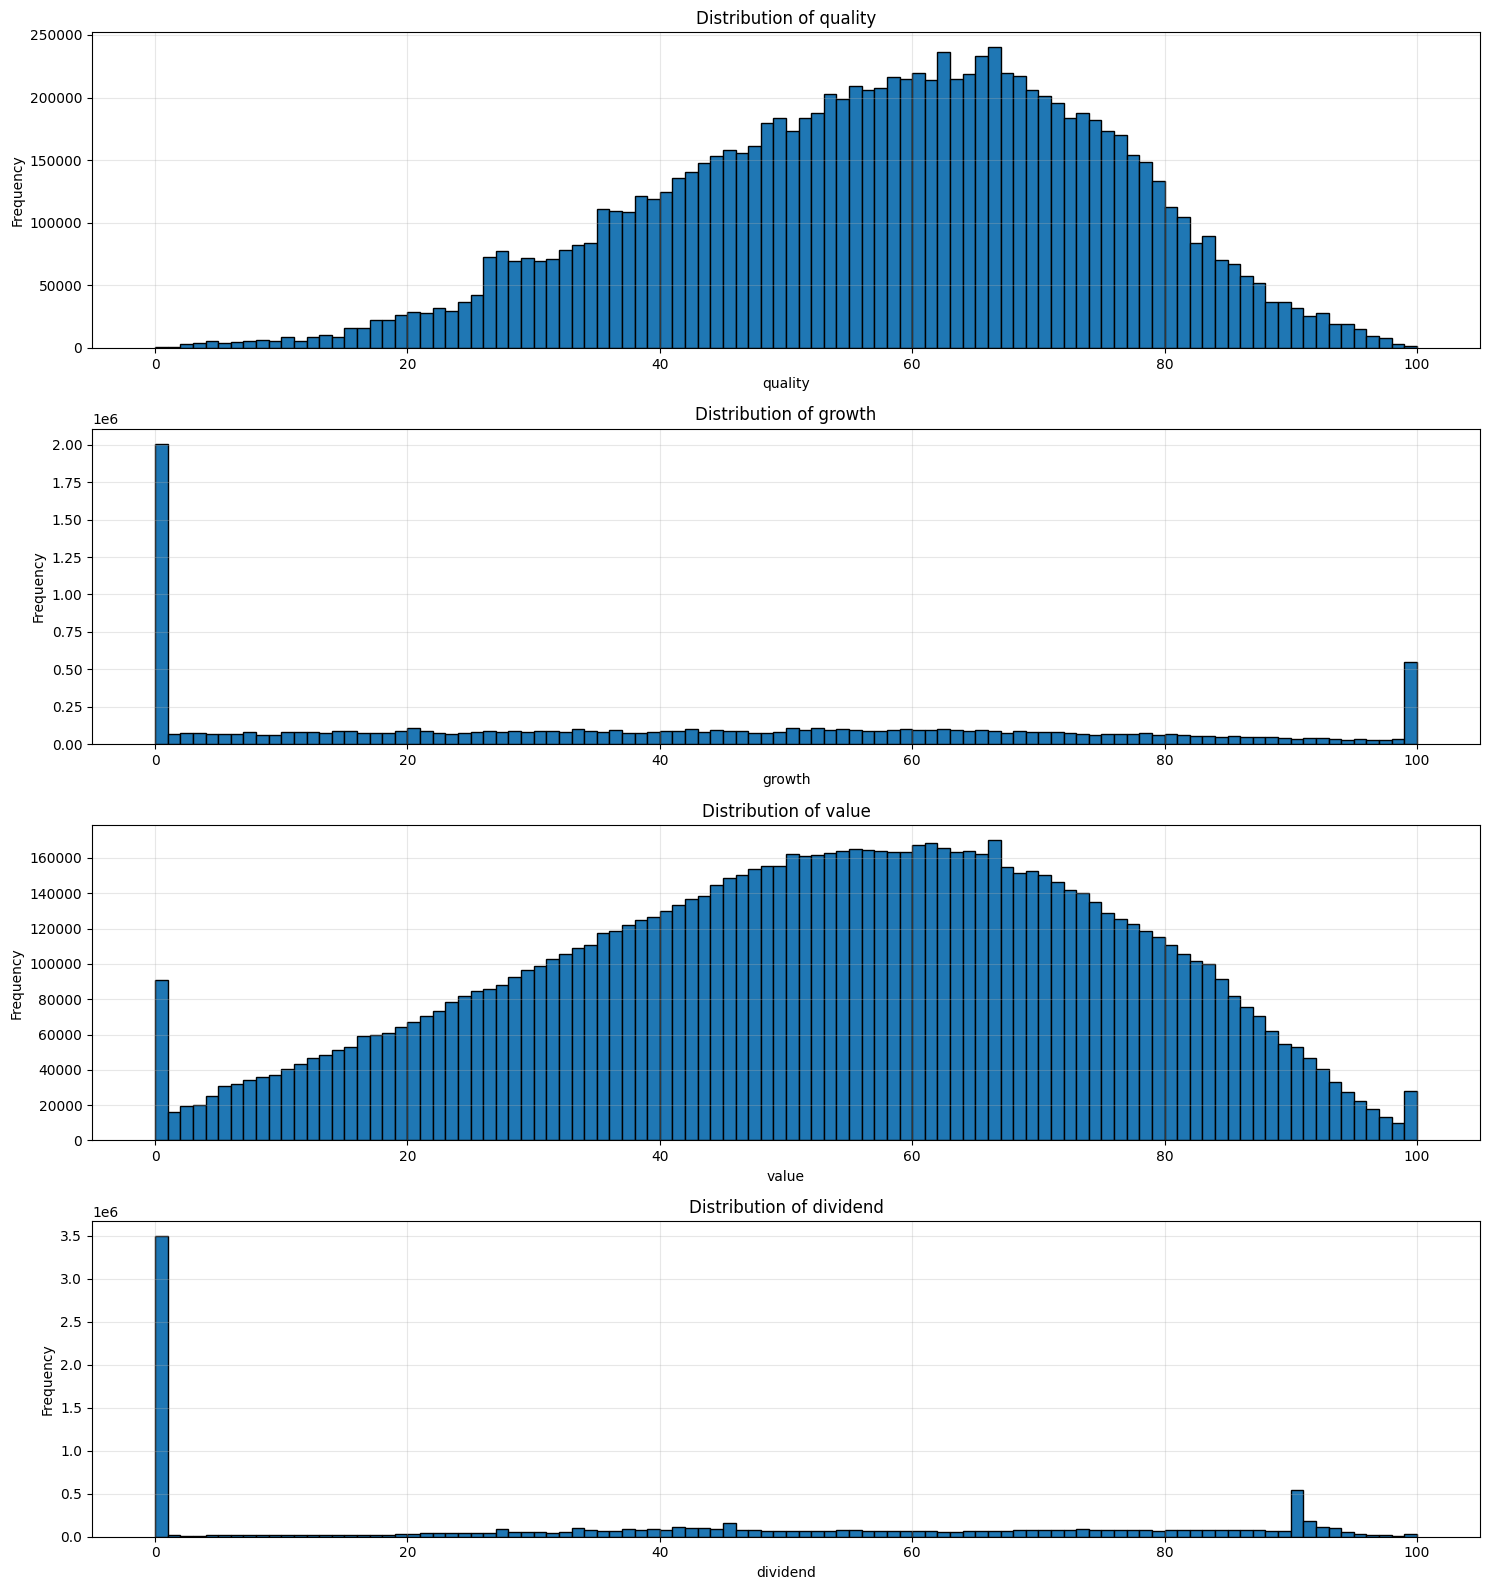
\includegraphics[width=0.8\textwidth]{images/code/descriptive analysis/distributions/Big Data past - Scores.png}
    \caption{Big Data Past - Scores}
    \label{fig:past_scores}
    \end{minipage}\hfill
    \begin{minipage}{0.48\textwidth}
        \centering
        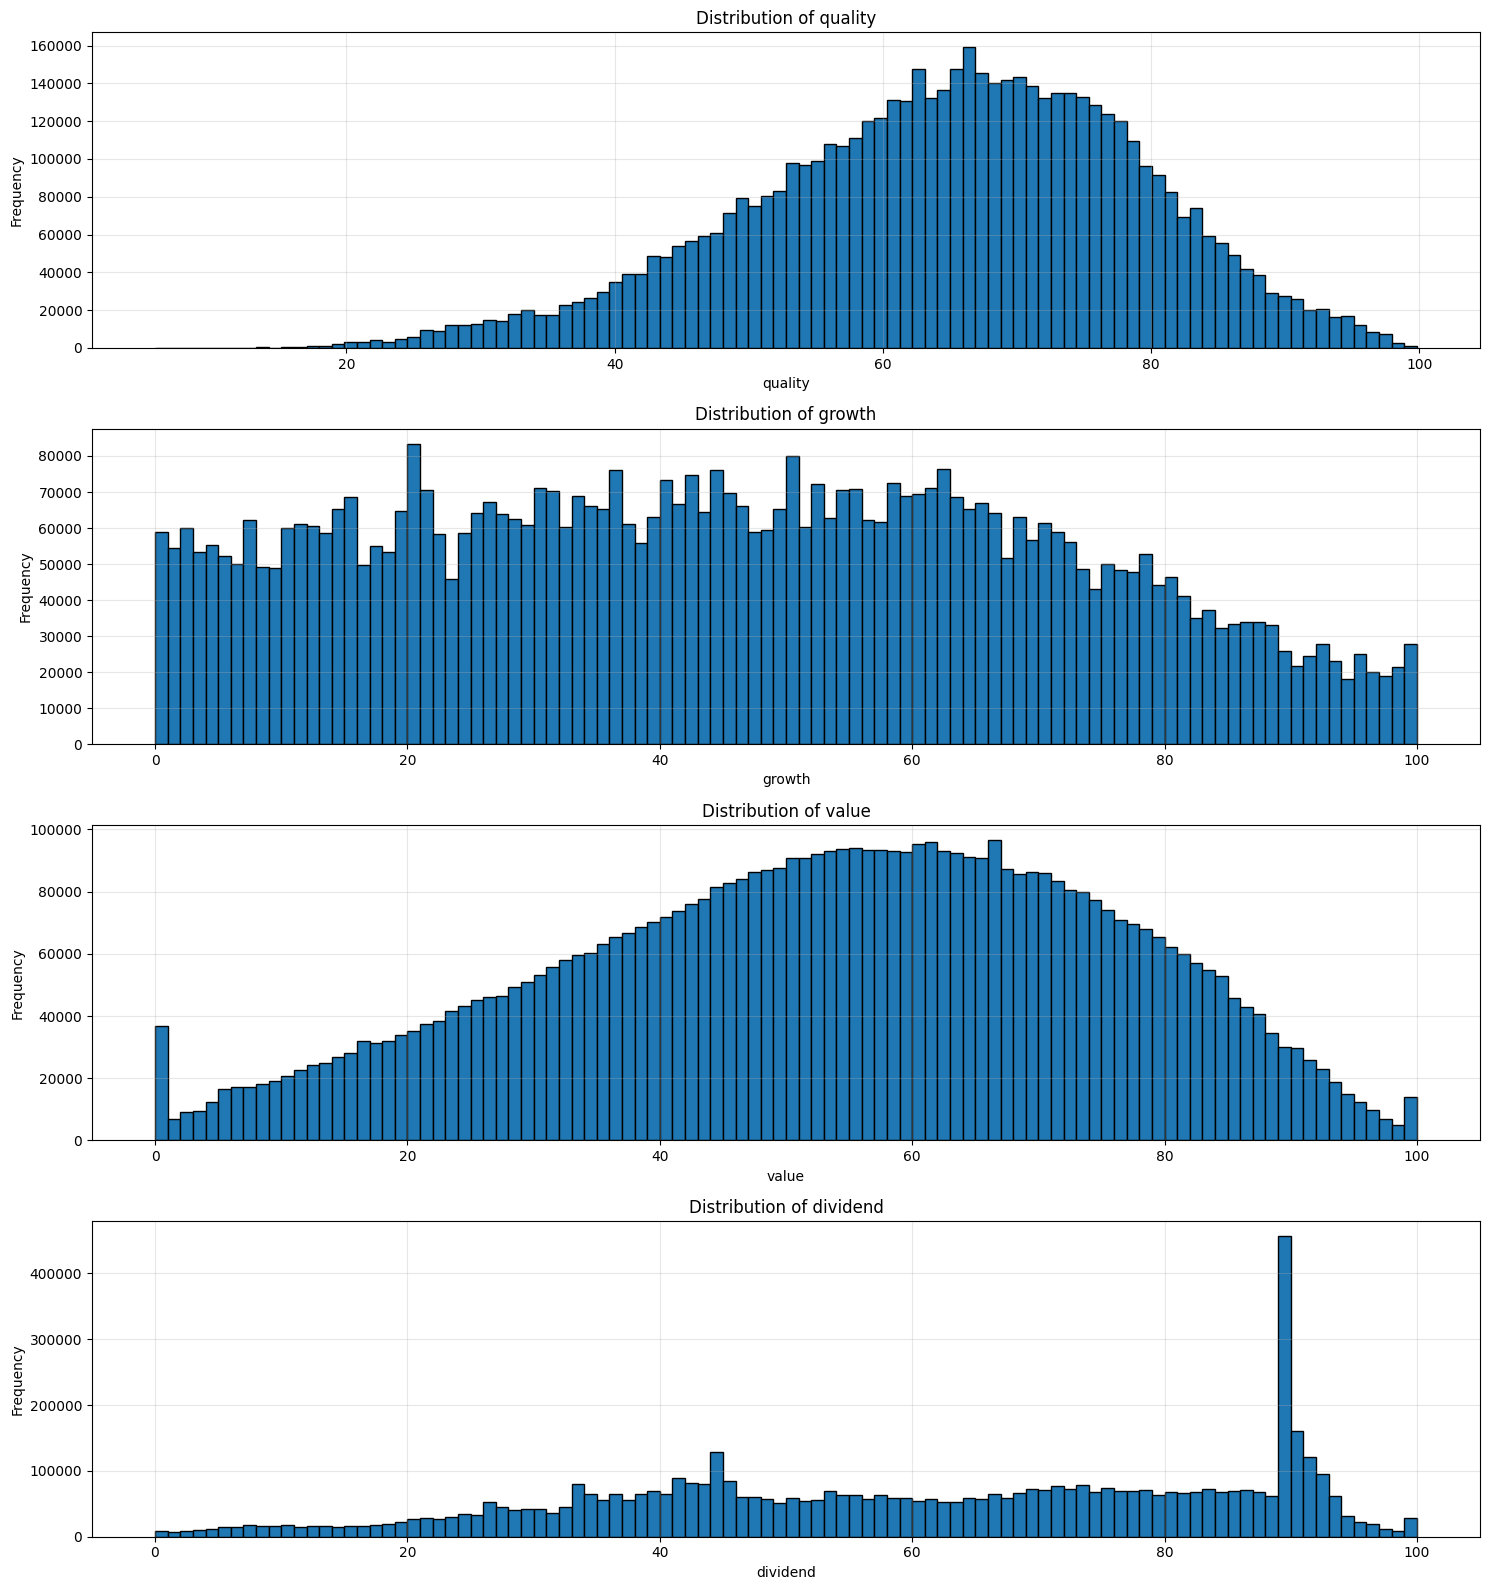
\includegraphics[width=0.8\textwidth]{images/code/descriptive analysis/distributions/Big Data past - Scores Deep.png}
        \caption{Big Data Past - Scores Deep}
        \label{fig:past_scores_deep}
    \end{minipage}
\end{figure}

\begin{figure}[H]
    \centering
    \begin{minipage}{0.48\textwidth}
        \centering
        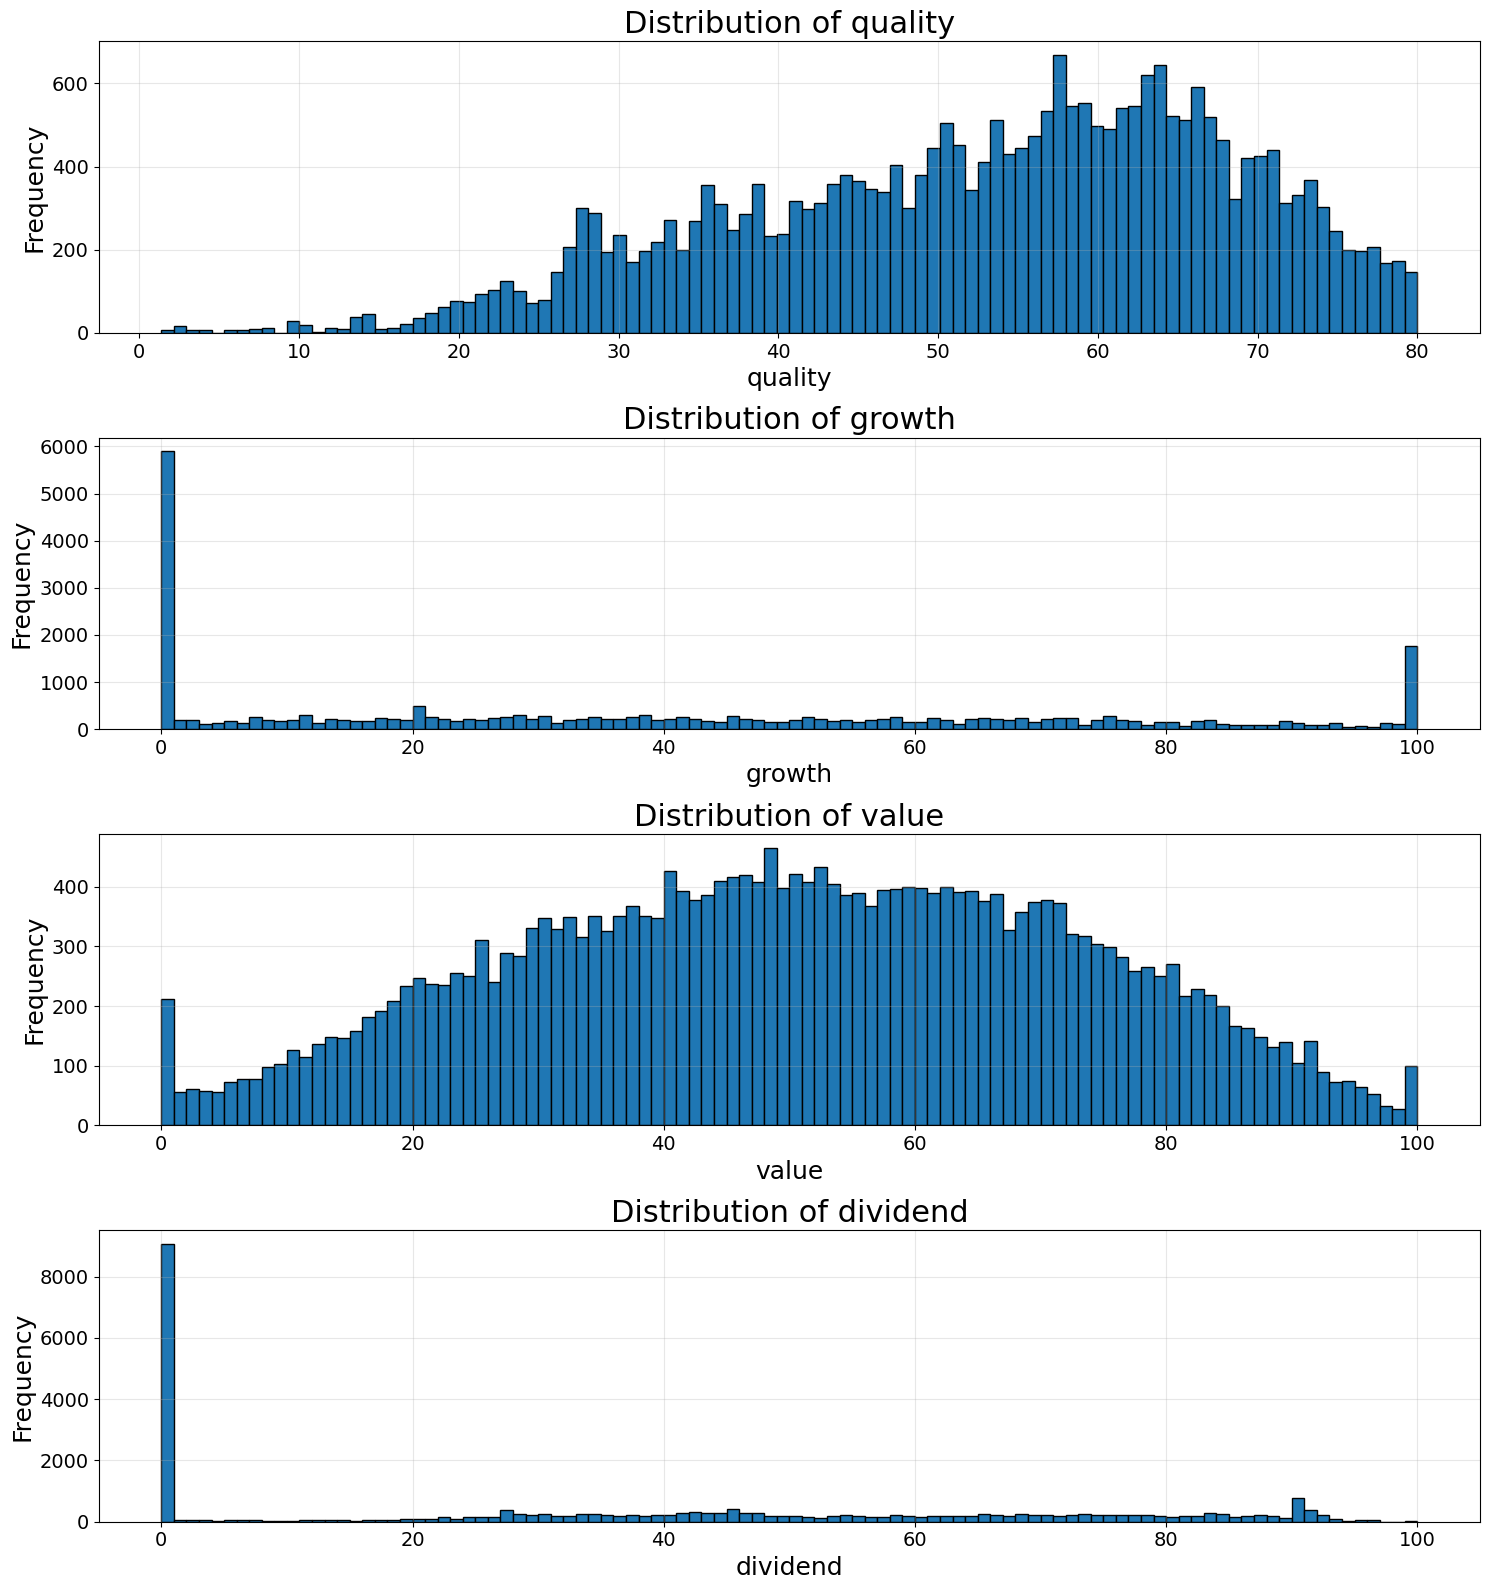
\includegraphics[width=0.8\textwidth]{images/code/descriptive analysis/distributions/Small Data future - Scores.png}
    \caption{Small Data Future - Scores}
    \label{fig:small_future_scores}
    \end{minipage}\hfill
    \begin{minipage}{0.48\textwidth}
        \centering
        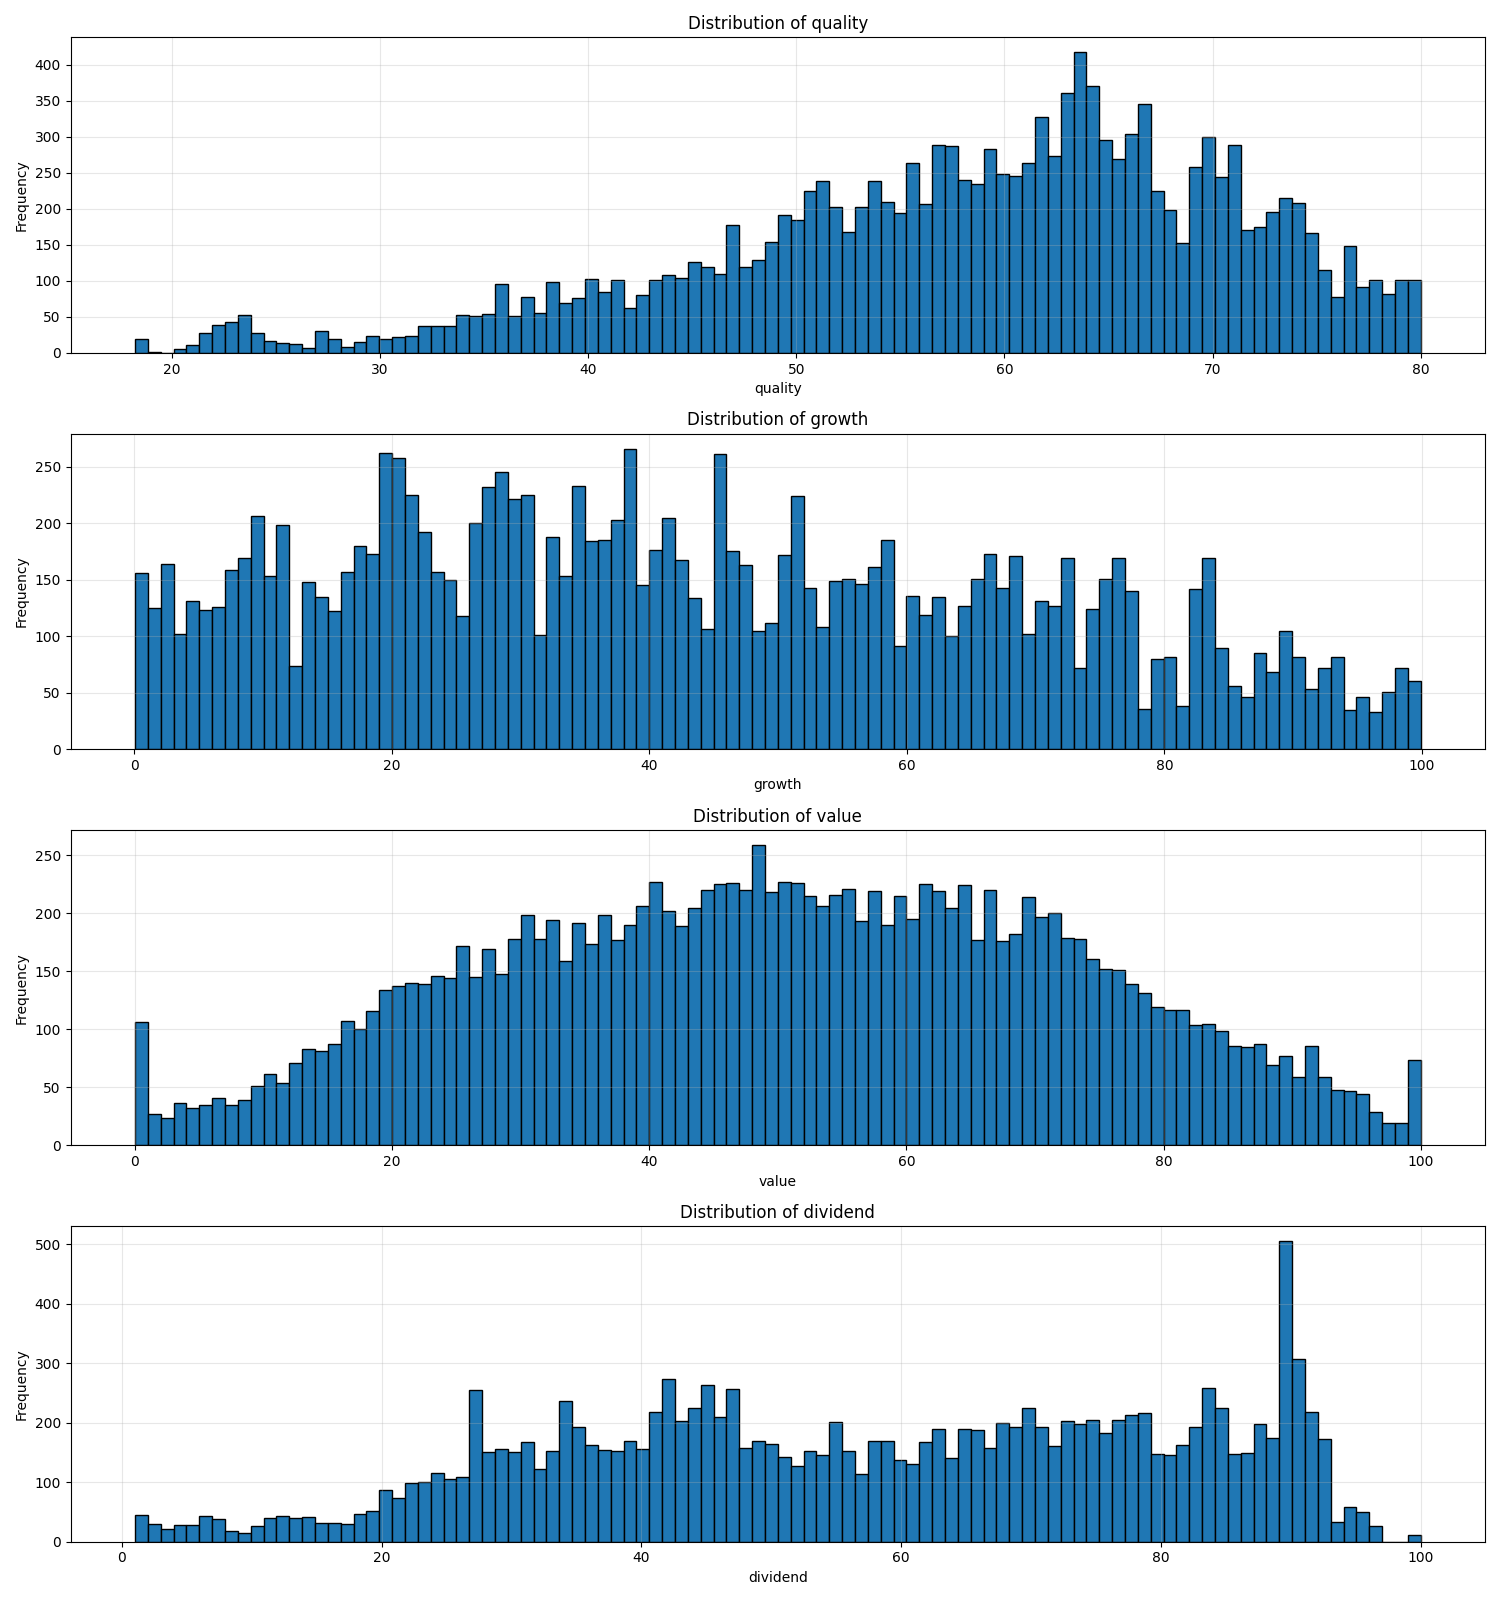
\includegraphics[width=0.8\textwidth]{images/code/descriptive analysis/distributions/Small Data future - Scores Deep.png}
        \caption{Small Data Future - Scores Deep}
        \label{fig:small_future_scores_deep}
    \end{minipage}
\end{figure}

\subsubsection{Dummies}

\begin{figure}[H]
    \centering
    \begin{minipage}{0.48\textwidth}
        \centering
        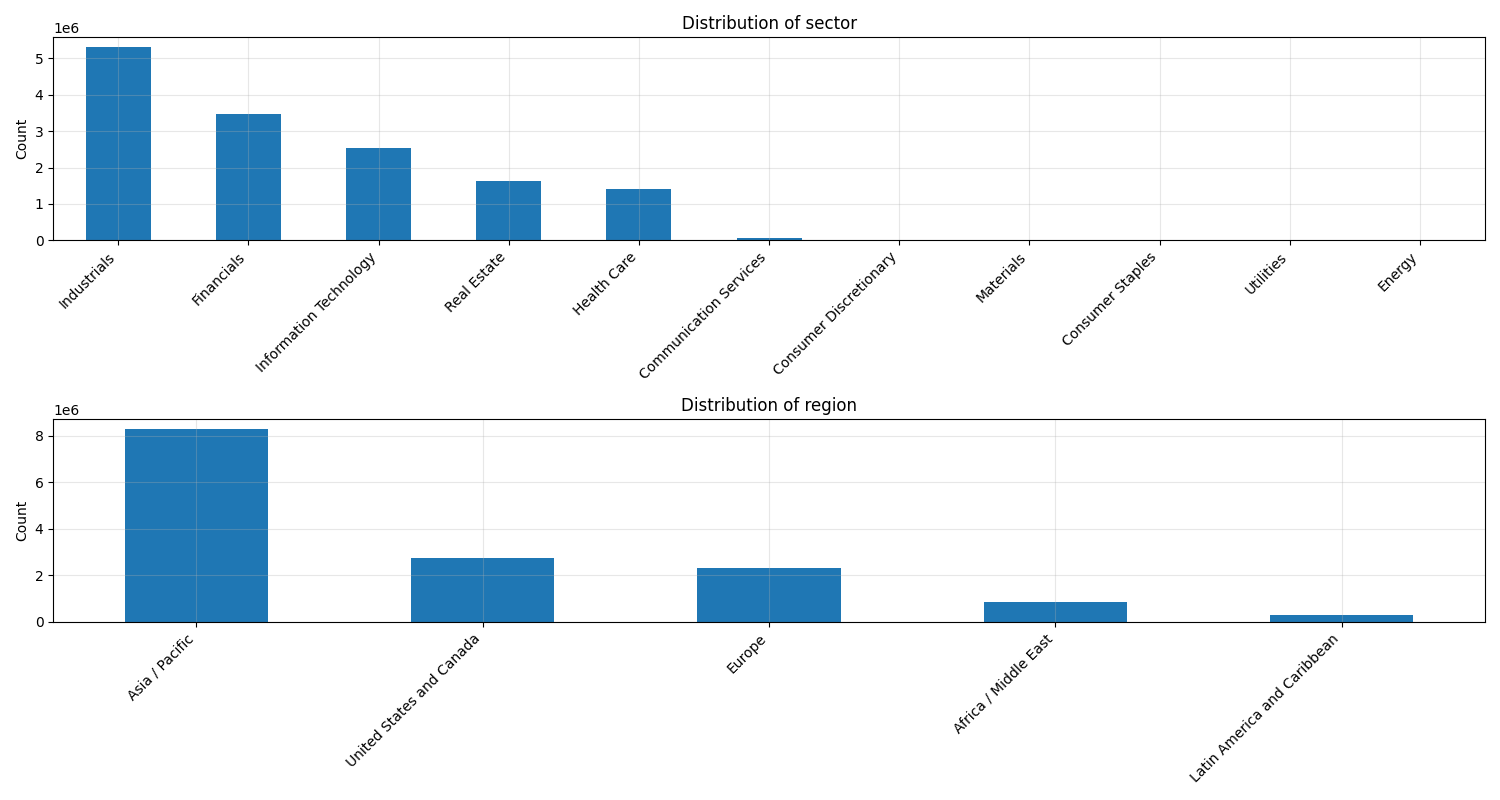
\includegraphics[width=0.8\textwidth]{images/code/descriptive analysis/distributions/Big Data future - Dummies.png}
    \caption{Big Data Future - Dummies}
    \label{fig:future_dummies}
    \end{minipage}\hfill
    \begin{minipage}{0.48\textwidth}
        \centering
        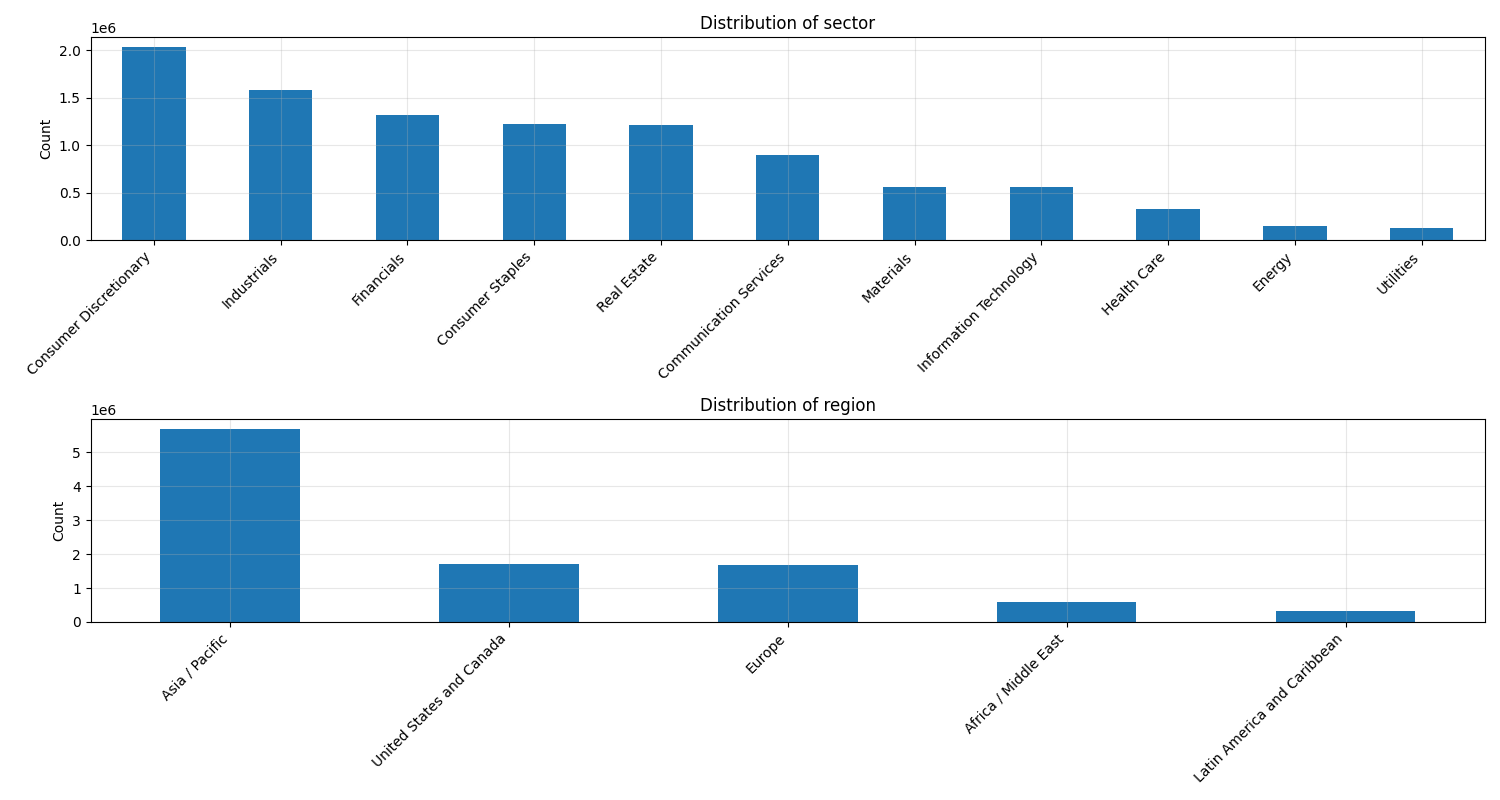
\includegraphics[width=0.8\textwidth]{images/code/descriptive analysis/distributions/Big Data past - Dummies.png}
        \caption{Big Data Past - Dummies}
        \label{fig:past_dummies}
    \end{minipage}
\end{figure}

\subsubsection{Profits}

\begin{figure}[H]
    \centering
    \begin{minipage}{0.48\textwidth}
        \centering
        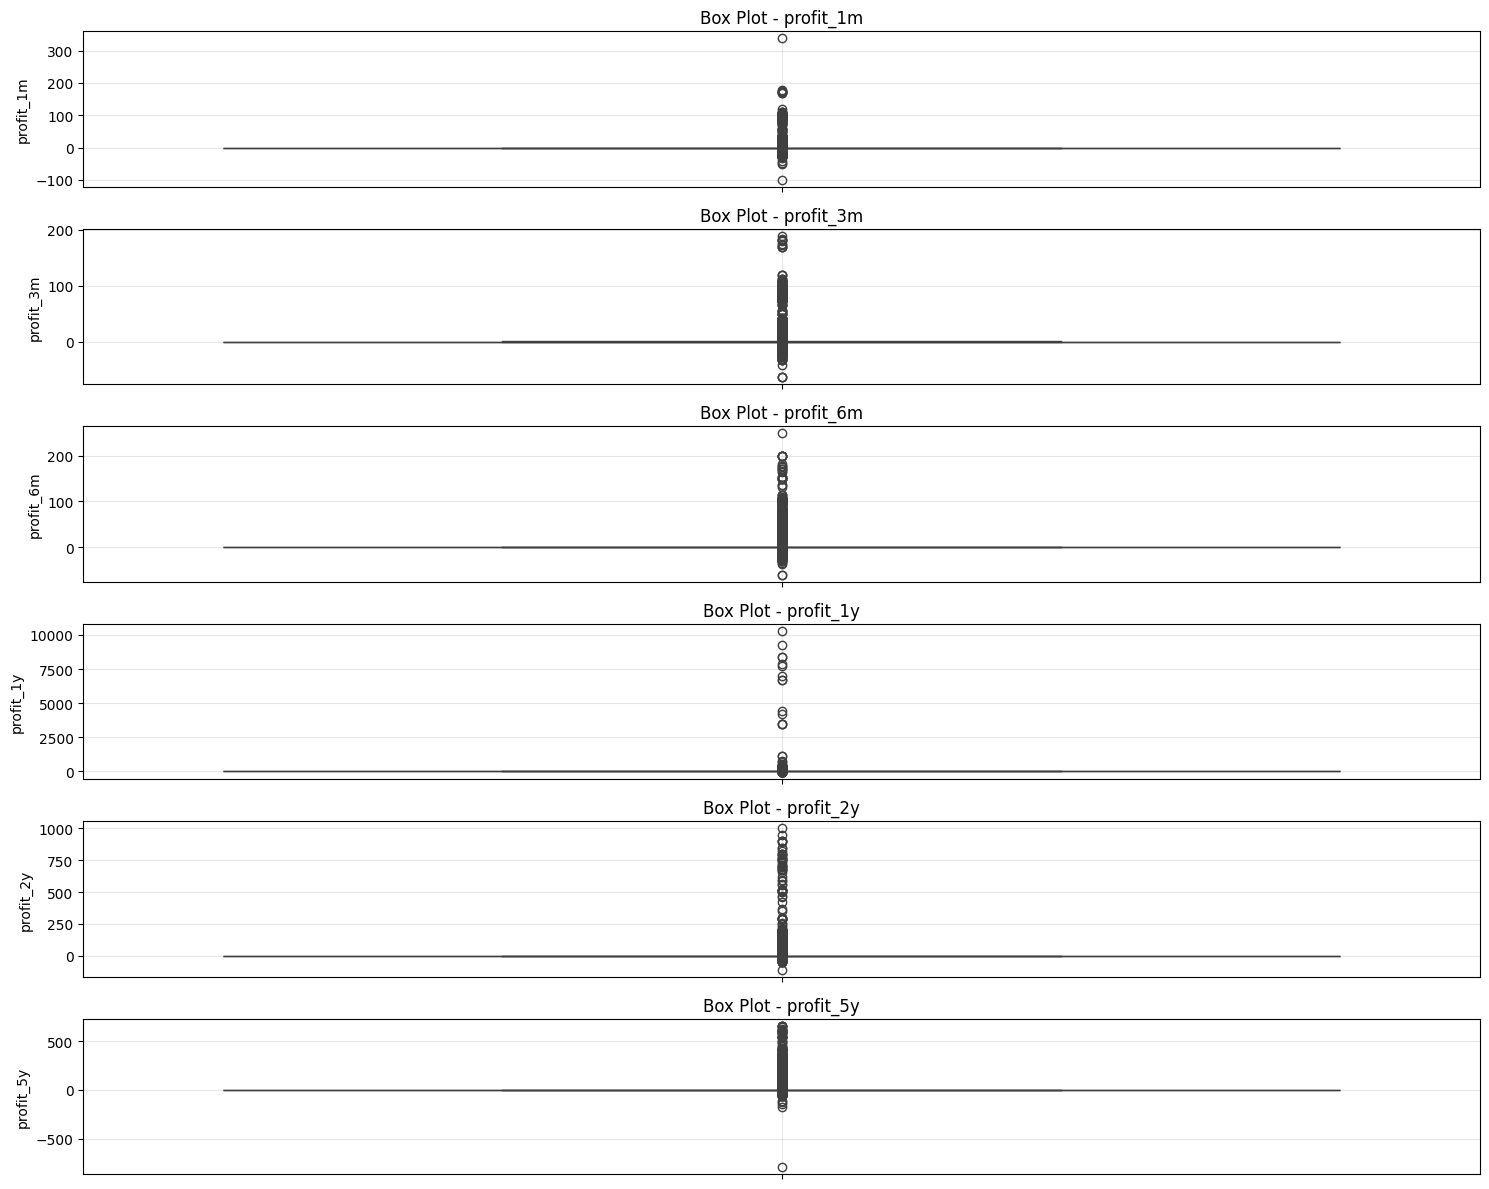
\includegraphics[width=\linewidth]{images/code/descriptive analysis/distributions/Big Data future - Profits Boxplot.png}
        \caption{Big Data Future - Profits Boxplot}
        \label{fig:big_data_future_profits_boxplot}
    \end{minipage}\hfill
    \begin{minipage}{0.48\textwidth}
        \centering
        \includegraphics[width=\linewidth]{images/code/descriptive analysis/distributions/Big Data Future - Profits.png}
        \caption{Big Data Future - Profits}
        \label{fig:big_data_future_profits}
    \end{minipage}
\end{figure}

\subsection{Correlations}

\subsubsection{USA and Canada}
\begin{figure}[H]
    \centering
    \begin{minipage}{0.48\textwidth}
        \centering
        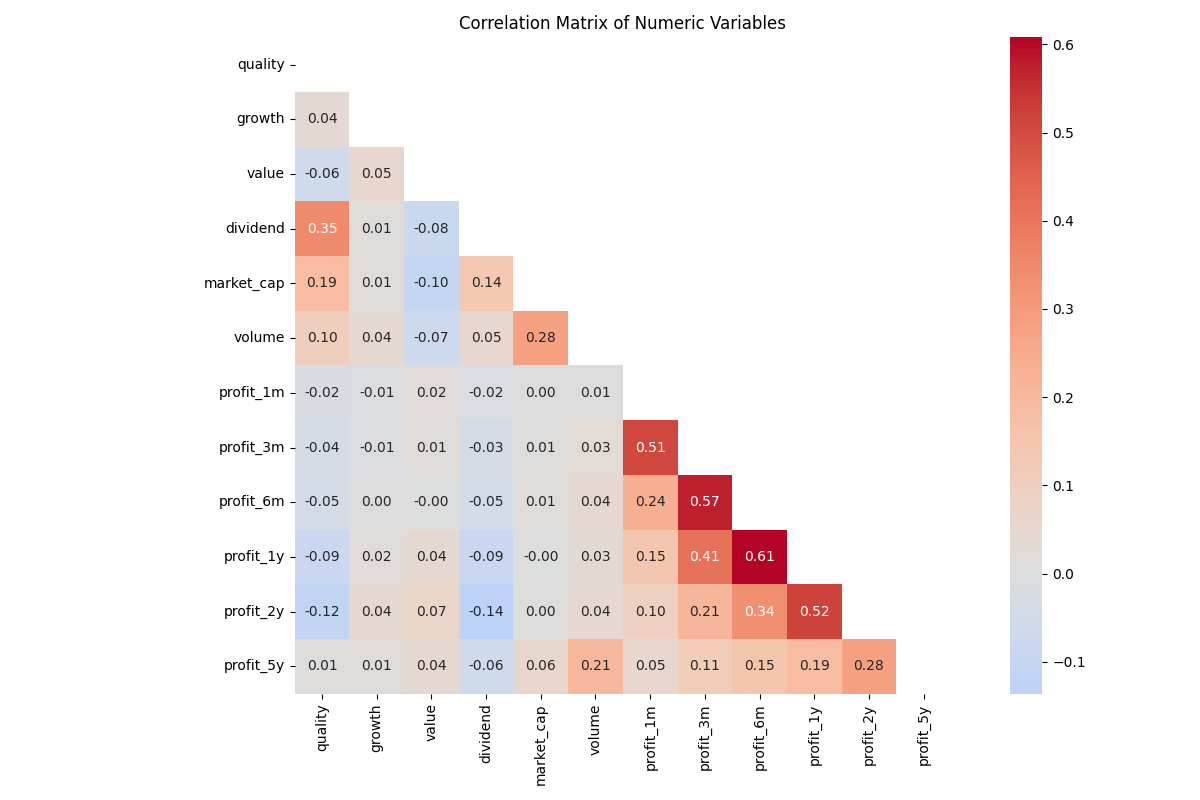
\includegraphics[width=\linewidth]{images/code/descriptive analysis/correlations/Small Data future USA.png}
        \caption{Small Data Future USA}
        \label{fig:small_data_future_usa_correlations}
    \end{minipage}
    \begin{minipage}{0.48\textwidth}
        \centering
        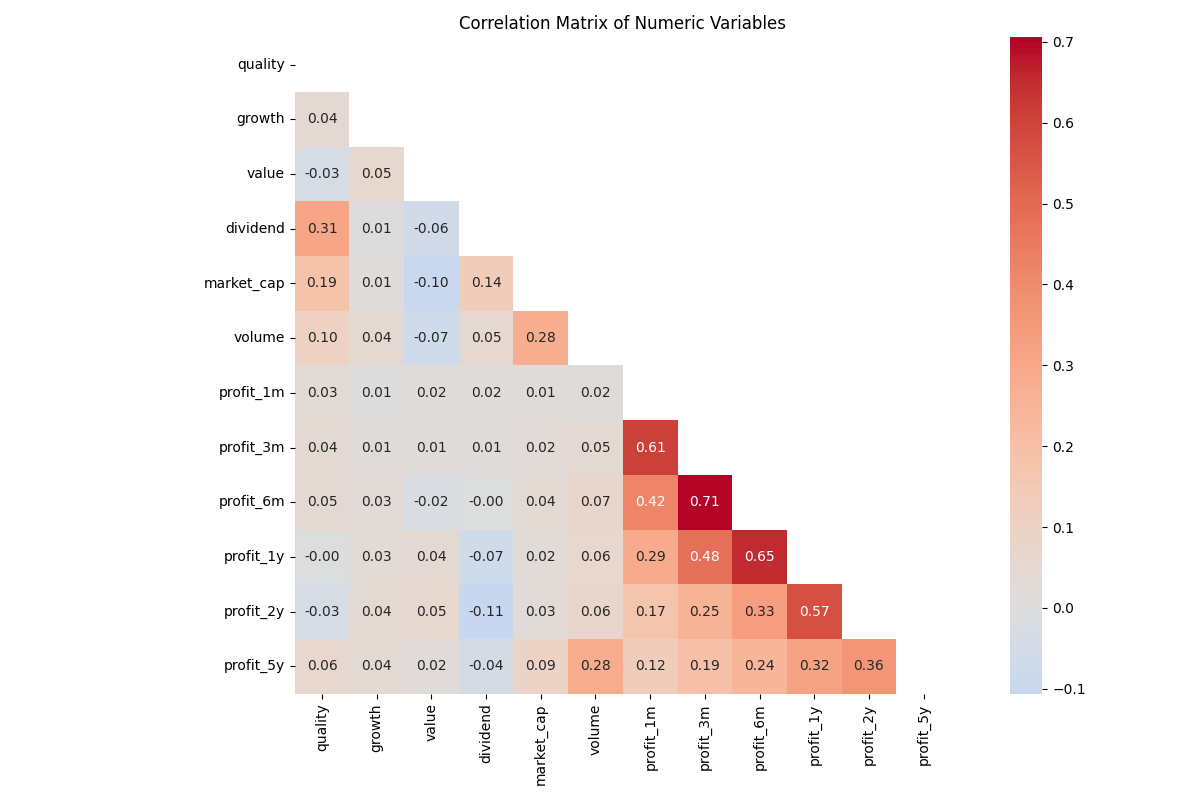
\includegraphics[width=\linewidth]{images/code/descriptive analysis/correlations/Small Data future USA - Multi.png}
        \caption{Small Data Future USA - Multi}
        \label{fig:small_data_future_usa_multi_correlations}
    \end{minipage}
\end{figure}

\subsubsection{Europe}
\begin{figure}[H]
    \centering
    \begin{minipage}{0.48\textwidth}
        \centering
        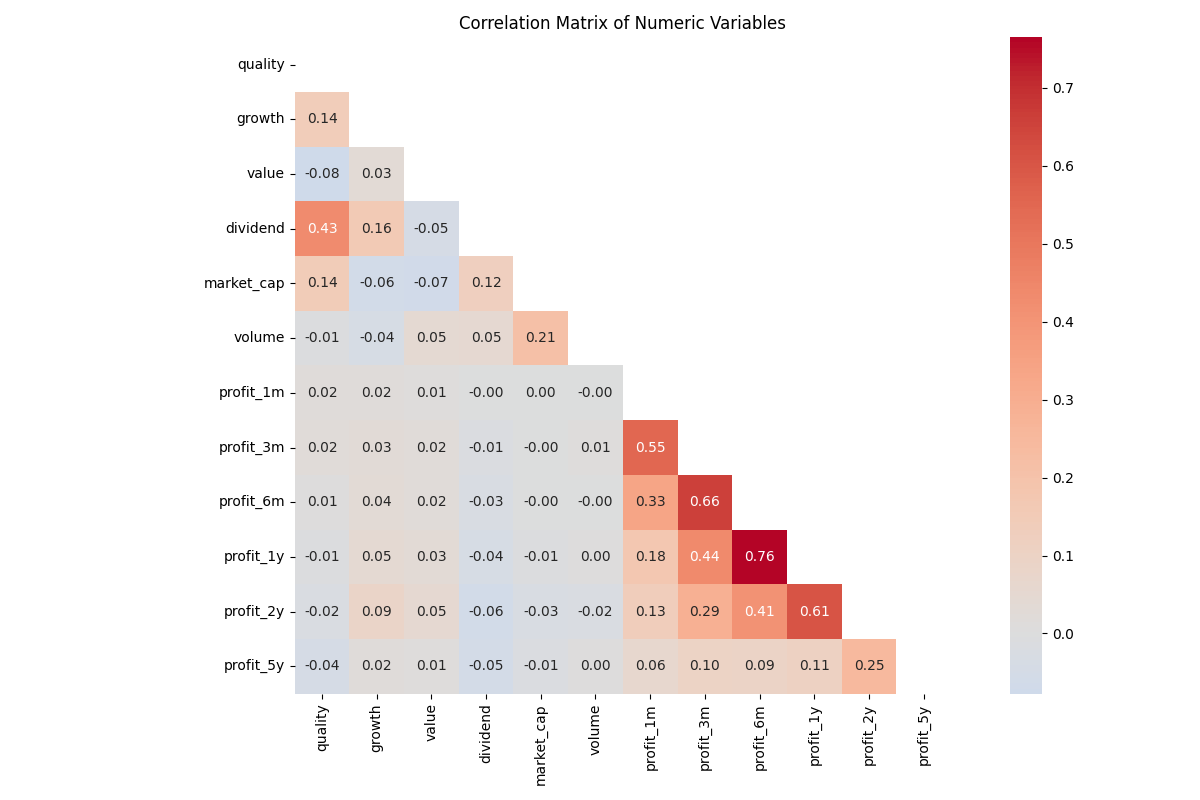
\includegraphics[width=\linewidth]{images/code/descriptive analysis/correlations/Small Data future EU.png}
        \caption{Small Data Future EU}
        \label{fig:small_data_future_eu_correlations}
    \end{minipage}
    \begin{minipage}{0.48\textwidth}
        \centering
        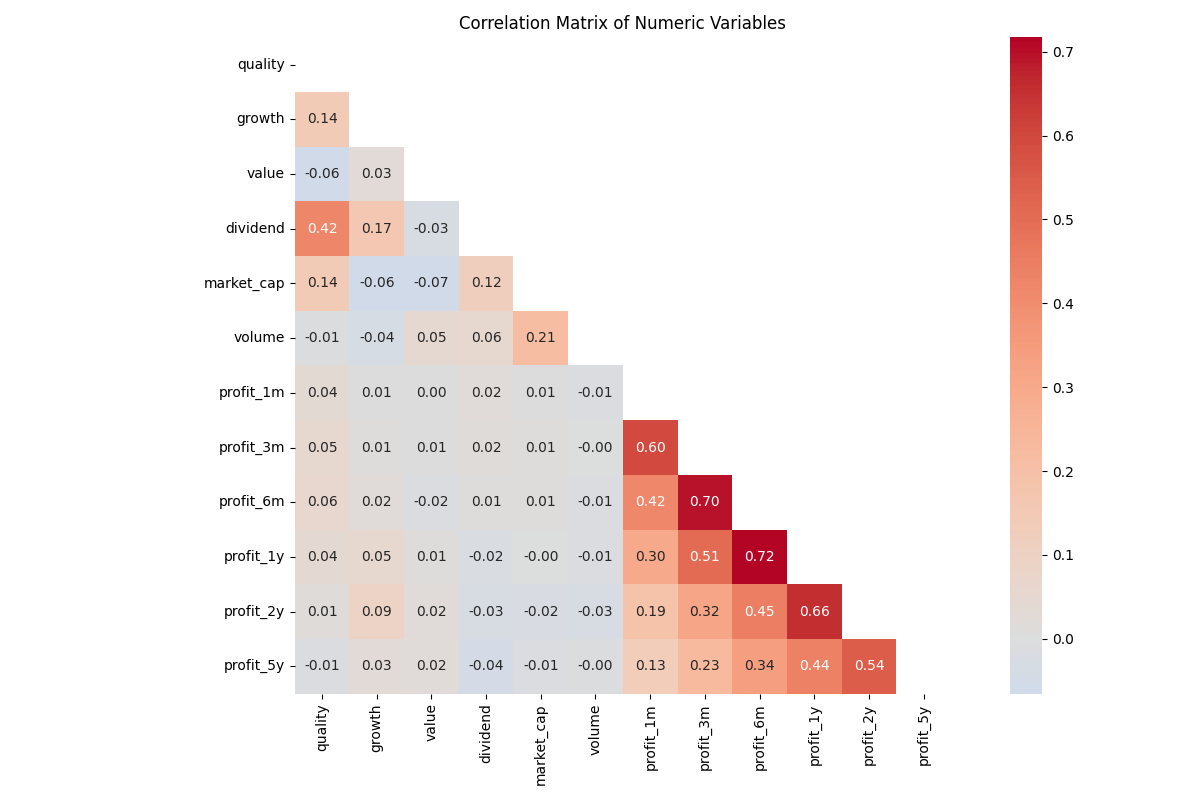
\includegraphics[width=\linewidth]{images/code/descriptive analysis/correlations/Small Data future EU - Multi.png}
        \caption{Small Data Future EU Multi}
        \label{fig:small_data_future_eu_multi_correlations}
    \end{minipage}
\end{figure}

\subsubsection{Latin America}
\begin{figure}[H]
    \centering
    \begin{minipage}{0.48\textwidth}
        \centering
        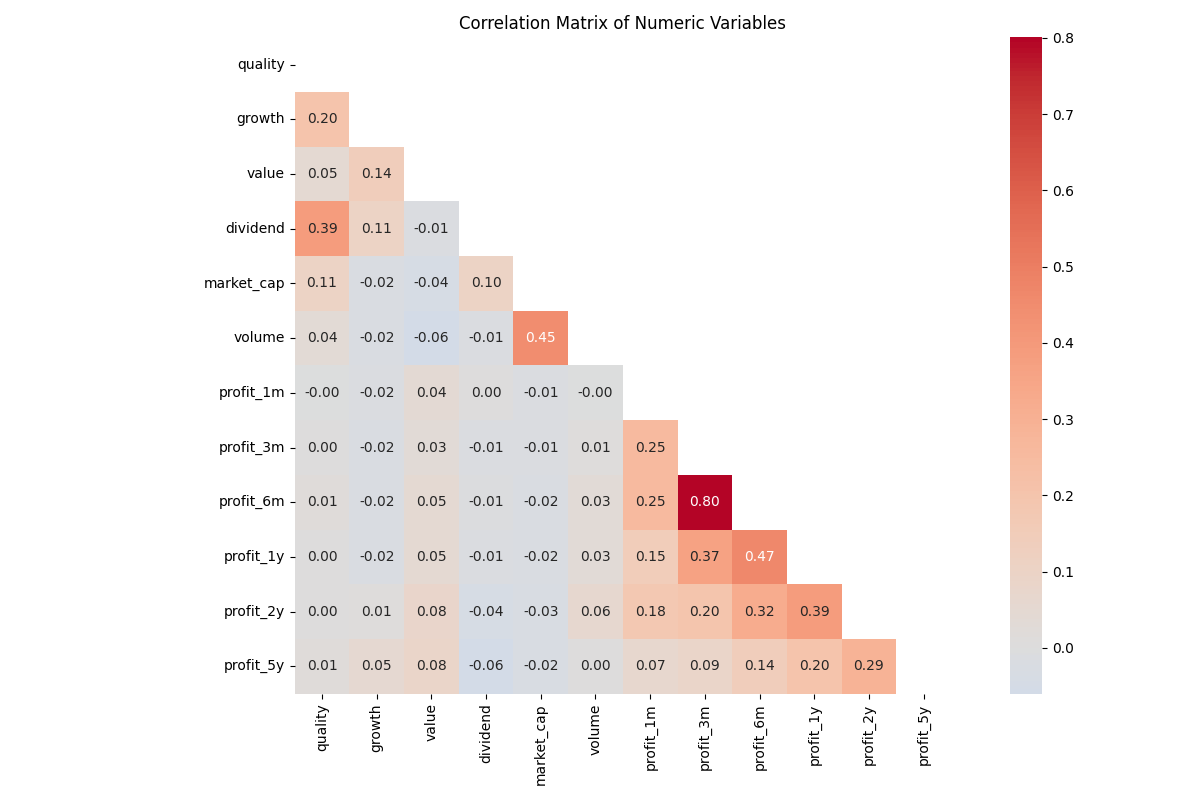
\includegraphics[width=\linewidth]{images/code/descriptive analysis/correlations/Small Data future LAT.png}
        \caption{Small Data Future LAT}
        \label{fig:small_data_future_lat_correlations}
    \end{minipage}
    \begin{minipage}{0.48\textwidth}
        \centering
        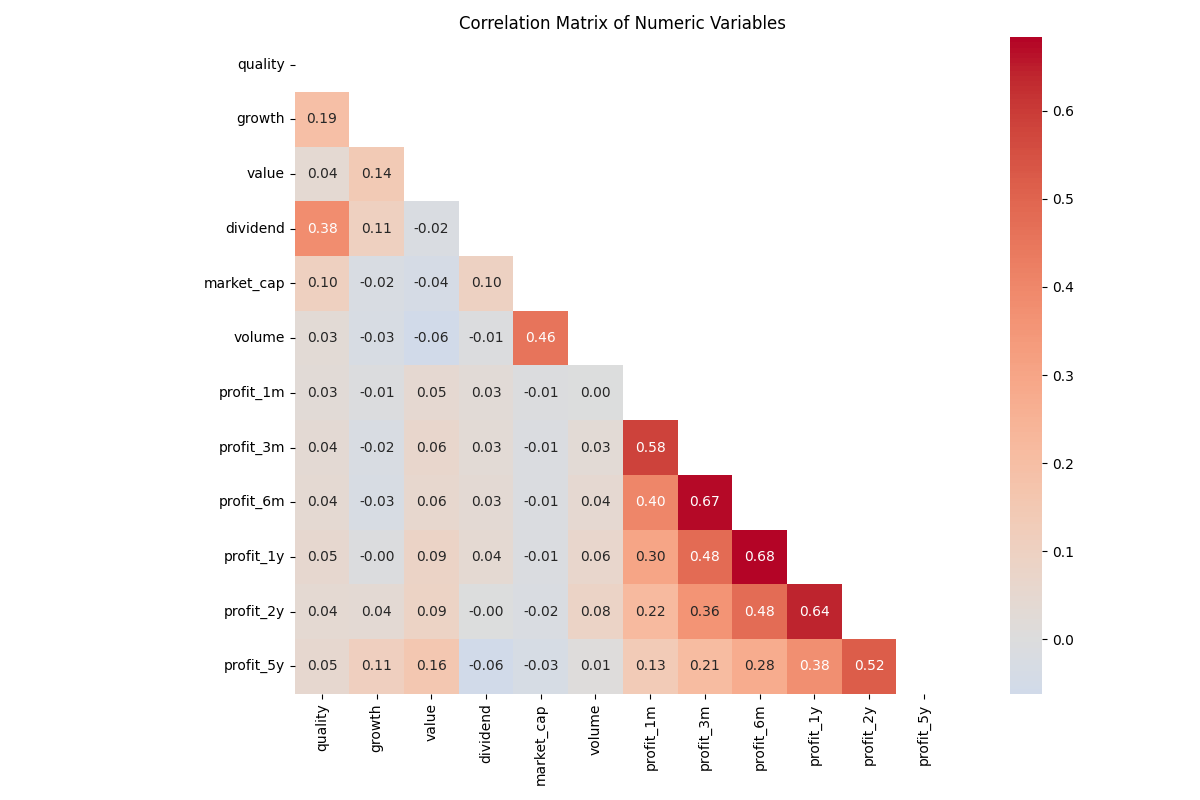
\includegraphics[width=\linewidth]{images/code/descriptive analysis/correlations/Small Data future LAT - Multi.png}
        \caption{Small Data Future LAT - Multi}
        \label{fig:small_data_future_lat_multi_correlations}
    \end{minipage}
\end{figure}

\subsubsection{Africa}
\begin{figure}[H]
    \centering
    \begin{minipage}{0.48\textwidth}
        \centering
        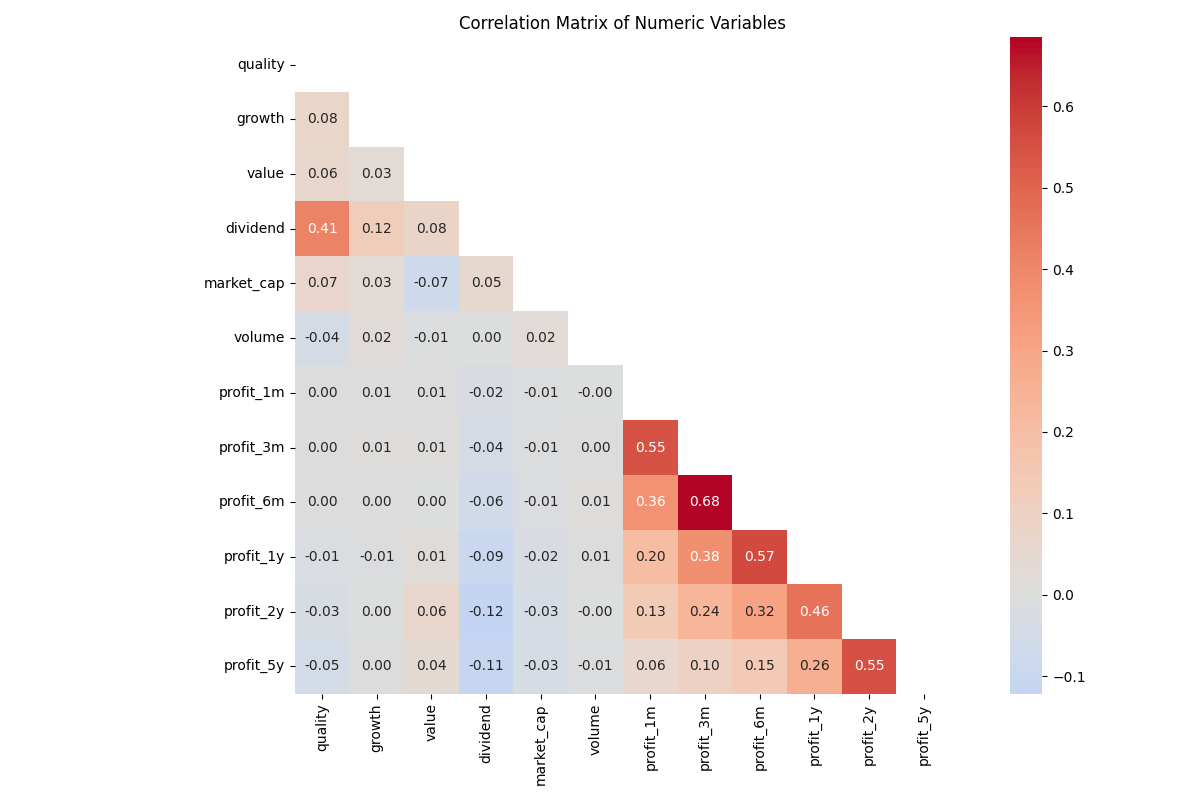
\includegraphics[width=\linewidth]{images/code/descriptive analysis/correlations/Small Data future AF.png}
        \caption{Small Data Future AF}
        \label{fig:small_data_future_af_correlations}
    \end{minipage}
    \begin{minipage}{0.48\textwidth}
        \centering
        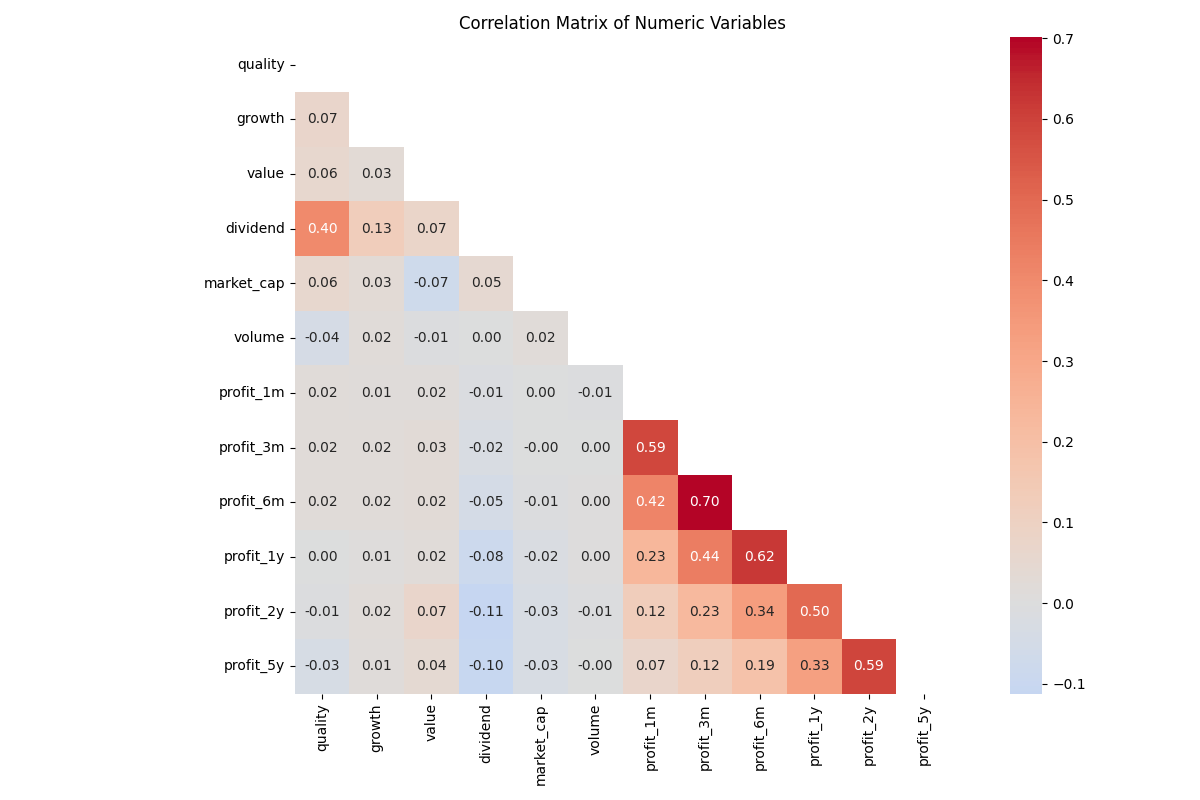
\includegraphics[width=\linewidth]{images/code/descriptive analysis/correlations/Small Data future AF - Multi.png}
        \caption{Small Data Future AF - Multi}
        \label{fig:small_data_future_af_multi_correlations}
    \end{minipage}
\end{figure}

\subsubsection{Asia and Oceania}
\begin{figure}[H]
    \centering
    \begin{minipage}{0.48\textwidth}
        \centering
        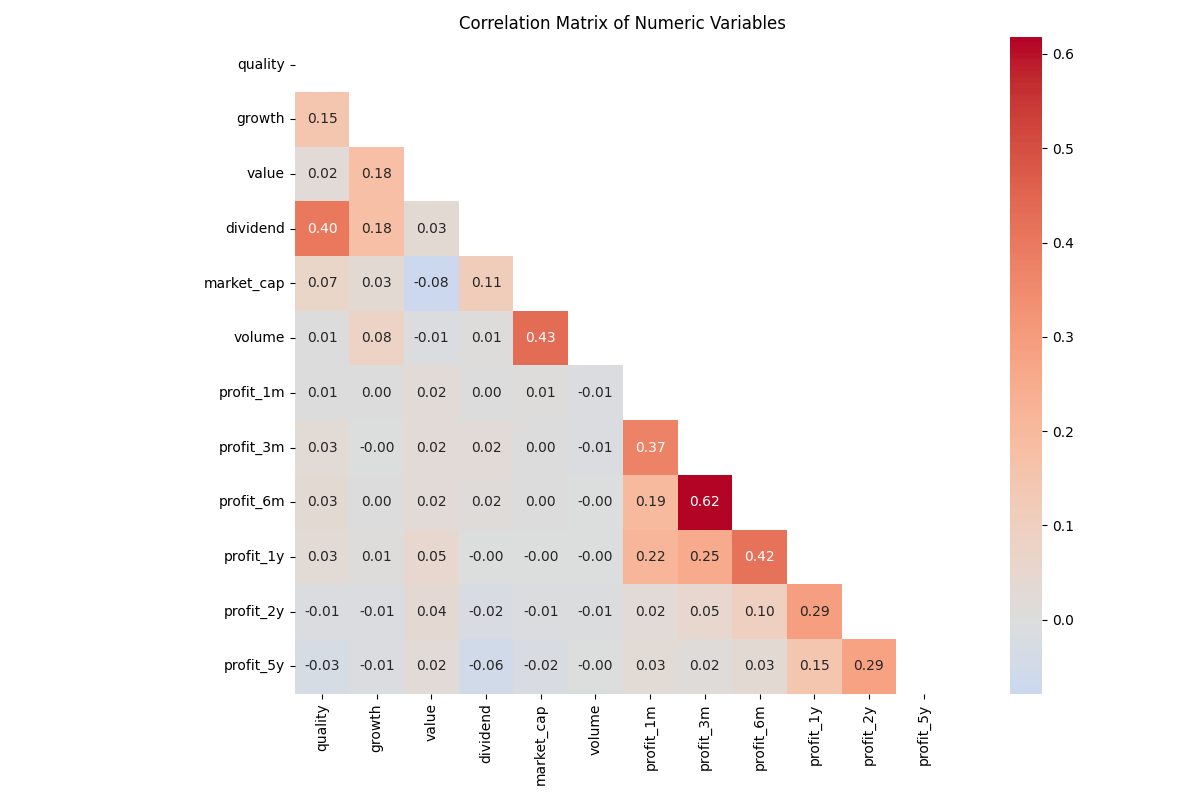
\includegraphics[width=\linewidth]{images/code/descriptive analysis/correlations/Small Data future AS.png}
        \caption{Small Data Future AS}
        \label{fig:small_data_future_as_correlations}
    \end{minipage}
    \begin{minipage}{0.48\textwidth}
        \centering
        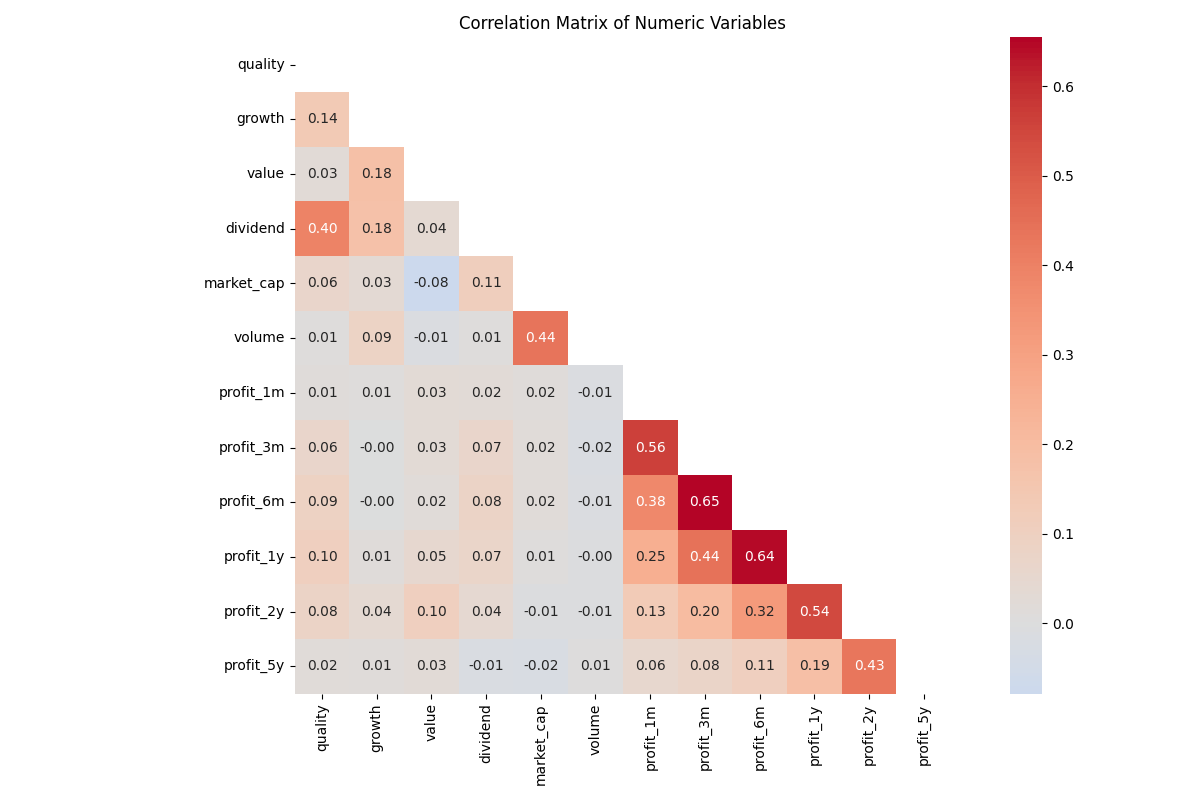
\includegraphics[width=\linewidth]{images/code/descriptive analysis/correlations/Small Data future AS - Multi.png}
        \caption{Small Data Future AS - Multi}
        \label{fig:small_data_future_as_multi_correlations}
    \end{minipage}
\end{figure}
\end{document}
